%TITULO------------------------------------------------------------------------

%==============================================================================
\chapter{Introdução}\label{introducao}
%==============================================================================

	%comentar sobre a conexão de conversores de tensão na rede e aplicações de filtragem
	%ativa. Depois, falar de geração distribuída e comentar problemas de harmônicas
	%de comutação

	A tensão fornecida pelo sistema elétrico de potência é idealmente senoidal e
	balanceada, com correntes de linha senoidais, amplitude e frequência fixas e
	fator de potência unitário. Durante a operação real do sistema, no entanto,
	é difícil manter as condições ideais. As divergências do padrão são classificadas
	como problemas de qualidade de energia e, por se tratarem de problemas, devem
	ser corrigidas.

	Problemas de qualidade de energia ocorrem com mais frequência e intensidade em
	ambientes industriais, devido ao tipo de carga instalada. Transformadores,
	fornos a arco, conversores tiristorizados e cargas semelhantes drenam correntes
	harmônicas e causam variações bruscas de energia reativa. É crescente a
	utilização de dispositivos eletrônicos de potência em equipamentos
	eletroeletrônicos, atualmente tão comuns em residências. Tais dispositivos possuem,
	em geral, um estágio de entrada sem correção do fator de potência, fazendo com que
	drenem correntes distorcidas da rede elétrica~\cite{ref:MANSOOR}. Estes fatores em
	conjunto agravam o problema de qualidade de energia, devido às suas consequências
	negativas, como	o aquecimento de condutores e transformadores devido à circulação
	de correntes reativas e o mau funcionamento de equipamentos sensíveis conectados
	ao sistema.	Tais consequências levaram à criação de normas internacionais que
	regulamentam limites para a distorção harmônica total, ou THD (do inglês \emph{
	Total Harmonic Distortion}). Como exemplos de normas pode-se citar a IEC 1000-3-2
	e a IEEE 519-1992.

	É possível mitigar estes problemas através da conexão de filtros de potência
	com a carga. Estes filtros podem ser ativos ou passivos, e a conexão pode ser
	em série, em paralelo, ou em série-paralelo. O filtro pode ser implementado
	com elementos passivos (resistores, indutores e capacitores) ou elementos
	ativos (chaves semicondutoras de potência), sendo os filtros ativos conhecidos
	como FAP's (Filtros Ativos de Potência). Embora filtros passivos sejam mais
	simples de projetar e mais baratos de construir do que filtros ativos, têm como
	desvantagem a possibilidade de oscilar com a impedância da linha e uma capacidade
	de compensação limitada, visto que para cada componente harmônica um reator
	deve ser projetado. Por isso, a partir da década de $70$, com o desenvolvimento
	da tecnologia de dispositivos semicondutores de potência, microprocessadores e
	processadores digitais de sinal, ou DSP's (do inglês \emph{Digital Signal
	Processor}) foi possível desenvolver algoritmos mais complexos de modulação,
	geração de referências e programas supervisórios, o que tornou a utilização de
	FAP's ainda mais popular~\cite{ref:SASAKI}.

	Além disso, diversos fatores têm levado à intensificação no uso de conversores
	eletrônicos	de potência nos últimos anos. As inúmeras aplicações que precisam de
	uma forma de conexão com a rede elétrica fazem uso de conversores de potência.
	Novas tecnologias, a crise energética e o aumento do efeito estufa são alguns dos
	motivos para o aumento desta demanda. Aplicações de geração distribuída, como
	células de energia,	painéis fotovoltaicos, turbinas eólicas e microturbinas são
	usadas não só para aumentar a energia disponível no sistema, mas também para
	melhorar sua confiabilidade, fornecendo energia aos consumidores mesmo durante
	uma falta na rede~\cite{ref:KARSHENAS}.	Na maioria destes geradores, a eletricidade
	está disponível em um estágio contínuo, ou é produzida em baixa frequência e,
	portanto, é convertida para um nível contínuo. Inversores de tensão são
	predominantemente utilizados para transferir energia de uma fonte contínua para
	a rede elétrica.

	Apesar de vastamente utilizados, os inversores de tensão demandam cuidado
	em sua utilização. Isso deve-se ao fato de o inversor de tensão trabalhar
	com uma frequência de comutação da ordem de kHz para manter as perdas de
	comutação em níveis aceitáveis. Para manter as correntes harmônicas oriundas
	do inversor em níveis aceitáveis, de forma a respeitar os códigos de
	rede, existem diversas topologias de filtro que podem ser
	utilizadas~\cite{ref:RIBEIRO}. A mais comum é a aplicação de um filtro L como
	interface entre a rede e o inversor. Mais recentemente, filtros LCL começaram
	a ser utilizados para esta função~\cite{ref:LINDGREN}\cite{ref:TEODORESCU}
	\cite{ref:XU}, pois apresentam maior atenuação das frequências harmônicas sem
	aumentar significativamente o consumo de potência reativa na frequência
	fundamental da rede quando comparados a filtros L~\cite{ref:FUCHS}. Além disso,
	as dimensões do filtro LCL são significativamente menores que a de um filtro L,
	reduzindo o custo do filtro e as perdas de operação.

	A indutância da rede pode ser considerada como parte do filtro LCL. No entanto,
	a incerteza quanto ao seu valor real altera a frequência de ressonância do
	filtro e pode levar a instabilidade. Por este motivo, a incerteza quanto ao
	valor da indutância da rede precisa ser incluída no projeto do
	controlador~\cite{ref:LISERRE}. Outro ponto importante é que o controlador
	precisa rejeitar distorções de corrente de baixa ordem resultantes da
	distorção de tensão no ponto de conexão do conversor. Isto, aliado ao fato de
	que o controlador é implementado em um microcontrolador ou um DSP, torna o
	projeto bastante complexo.

	Por ser de terceira ordem, o filtro LCL apresenta um pico de amplitude em
	sua frequência de ressonância, o que faz com que a estabilidade geral do
	sistema seja reduzida dependendo principalmente de sua frequência de
	ressonância. Dessa forma, é necessário realizar o amortecimento desta
	ressonância. É possível realizar este amortecimento de forma passiva
	através da inserção	de um resistor em série ou em paralelo com o capacitor
	do filtro~\cite{ref:AHMED}. Embora este amortecimento reduza consideravelmente
	o pico de amplitude na frequência de ressonância, ele resulta em dissipação de
	energia pelo filtro e degrada o desempenho de atenuação nas altas frequências. Não é,
	portanto, uma solução aceitável para aplicações que necessitam do máximo de
	desempenho~\cite{ref:SHEN}. Outra forma de realizar este amortecimento é via
	amortecimento ativo~\cite{ref:GERVASIO}. Isto é alcançado utilizando uma dentre
	várias estratégias de controle possíveis, tais como estruturas de controle
	específicas~\cite{ref:WU}, estimação de impedância da rede~\cite{ref:BLAABJERG},
	retroação de estados~\cite{ref:MASSING}, estratégias utilizando múltiplos laços de
	realimentação~\cite{ref:POH}, dentre outras~\cite{ref:WESSELS} \cite{ref:MORENO}
	\cite{ref:YANG}.

	Em geral, essas estratégias de controle podem ser implementadas analogicamente ou
	digitalmente. Os métodos de controle digital oferecem diversas vantagens sobre
	as técnicas analógicas, como reprogramabilidade, tolerância à variações
	nos componentes, suporte a multiplos modos de operação, melhor eficiência e,
	em geral, melhor desempenho. O controle analógico se limita a estruturas particulares,
	enquanto o controle digital depende apenas dos limites da taxa de amostragem,
	resolução e capacidade computacional~\cite{ref:KIMBALL}.

	Assim sendo, o enfoque recai sobre as técnicas de controle digital. Existem
	muitas técnicas diferentes para o controle de conversores. O controle
	proporcional-integral, comumente chamado de PI, utiliza compensadores de
	erro do tipo proporcional-integral para produzir os sinais de comando de
	cada fase. A parte integral do controlador minimiza o erro em baixas
	frequências, enquanto a parte proporcional e a posição do zero
	influenciam na ondulação do sinal. O desafio desta técnica é realizar o
	rastreamento das referências de corrente. Isto é resolvido, em geral,
	utilizando circuitos do tipo malha de captura de fase, ou PLL (do inglês
	\emph{Phase Locked Loop}) para gerar as referências de corrente. O controlador
	PI geralmente é implementado em eixos síncronos dq, de modo que as
	referências senoidais são transformadas em sinais constantes. Alternativamente,
	podem ser utilizados PI em eixos estacionários
	$\alpha \beta$~\cite{ref:KAZMIERKOWSKI}. Em ambos os casos, o objetivo é o
	rastreamento de referências senoidais e a rejeição de distúrbios de mesma
	natureza~\cite{ref:AREERAK}.

	Uma outra abordagem é o controle de corrente usando um controlador do tipo
	\emph{Dead-Beat}. Essa é a mais rápida estratégia de controle linear que pode
	ser adotada. Teoricamente, o laço de corrente replica exatamente a corrente
	de referência com dois ciclos de atraso. O controle é baseado no modelo interno
	do sistema, usado para prever o comportamento dinâmico do sistema. O
	controlador, assim sendo, é inerentemente sensível às incertezas do
	modelo~\cite{ref:MALESANI}.

	Existe ainda o controlador por Histerese. Devido à sua inerente não-linearidade,
	este controlador é capaz de proporcionar uma resposta dinâmica rápida.
	Utilizando esta técnica, é possível atingir o máximo aproveitamento do conversor
	de potência~\cite{ref:YAO}. O limite para a regulação de corrente, na verdade,
	é dado pelo projeto do conversor. O controle de corrente por histerese é estável
	e robusto com relação à variações na carga ou qualquer outro tipo de distúrbios
	dinâmicos~\cite{ref:TENTI}.

	O controle de realimentação é a estratégia de controle mais simples que existe
	para compensar perturbações de um processo. Embora a grande maioria das estratégias
	de controle utilizadas na prática industrial seja controle de realimentação simples,
	essa estratégia apresenta uma desvantagem bastante significativa: é preciso que
	um distúrbio se propague pelo processo, fazendo a variável controlada desviar
	do ponto de operação, para que a realimentação adote uma ação corretiva~\cite{ref:SMITH}.

	Existem aplicações, no entanto, que demandam desempenho superior, devido à alguma
	necessidade específica, dinâmica lenta ou perturbações frequentes. Quando o distúrbio
	é associado à variável controlada ou quando o elemento de controle final apresenta
	comportamento não-linear, o Controle Multimalha melhora significativamente o
	desempenho em relação ao controle com realimentação simples~\cite{ref:KRISHNA}.

	Este tipo de controle pressupõe um conjunto de malhas em cascata, onde as mais
	externas geram as referências para as malhas mais internas. Dessa forma, variáveis
	intermediárias são usadas para reduzir o efeito de algumas dinâmicas no processo.
	Não é mais necessário esperar o distúrbio propagar-se pelo sistema e modificar a
	variável controlada. Uma vez que uma mudança seja detectada em uma variável
	intermediária, a ação corretiva começa imediatamente a ser aplicada na variável
	manipulada, reduzindo a magnitude do impacto do distúrbio e consequentemente
	melhorando o desempenho. O único requisito para que isto aconteça é que a malha
	interna seja mais rápida que a malha externa. Quanto mais rápida, melhor, pois
	a velocidade da malha interna implica na velocidade com que mudanças na variável
	intermediária serão detectadas, o que afeta diretamente a redução do impacto
	do distúrbio na variável controlada.

	As técnicas de controle clássicas pressupõe o uso de um modelo interno do sistema
	que deve ser precisamente conhecido. Nas duas últimas décadas, este requisito
	vem sendo relaxado, e o desafio é desenvolver estratégias de controle robustas
	à incerteza paramétrica~\cite{ref:GEROMEL}.

	%Considerando o contexto descrito acima, a proposta desse trabalho é apresentar
	%uma estratégia de controle de conversores conectados à rede elétrica através de
	%um filtro LCL. Esta estratégia apresenta ótimo desempenho através do uso de
	%Controle Multimalha, é capaz de rejeitar distúrbios e é robusta em relação à
	%incertezas paramétricas em termos da indutância da rede.

\section{Considerações sobre \emph{LCL}}

    A principal vantagem do filtro LCL sobre o filtro L é conseguir uma melhor
    atenuação das componentes harmônicas de corrente oriundas do processo de comutação do
    conversor utilizando componentes indutivos de menor volume. Isto é obtido pela
    inserção de um capacitor, resultando num filtro do tipo \emph{T}~\cite{ref:SHEN}.
    Para análise, considere a estrutura da Fig.~\ref{fig:LCL_topologia}. Os indutores
    $L_1$ e $L_2$ e o capacitor $C$ formam o filtro LCL, com suas resistências
    associadas $R_1$, $R_2$ e $R_d$ respectivamente. A indutância $L_g$ e sua
    resistência associada $R_g$ correspondem à indutância da rede, $V_i$
    é a tensão de saída do inversor e $V_g$ é a tensão da rede:

    \begin{figure}[htb]
        \centering{
            %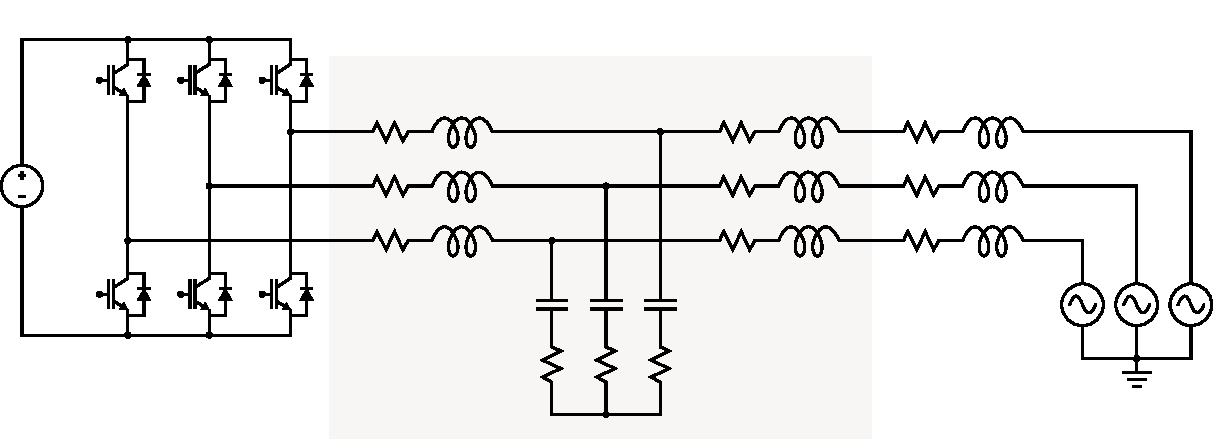
\includegraphics[width=0.9\textwidth]{img/topologia}}
            \def\svgwidth{\textwidth}
            \input{./img/topologia.pdf_tex}}
        \renewcommand\figurename{Fig.}
        \caption{Topologia do filtro LCL.}
        \label{fig:LCL_topologia}
    \end{figure}

    Dessa forma, tem-se:

    \begin{equation*}
        Z_i = L_1s +R_1
    \end{equation*}

    \begin{equation*}
        Z_g = (L_2 + L_g)s + R_2 + R_g
    \end{equation*}

    \begin{equation*}
        Z_0 = \frac{1}{Cs} + R_d
    \end{equation*}

    Pode-se definir então, as seguintes funções de transferência:

    \begin{equation}
        G_{V_i-I_1}(s) = \frac{I_1(s)}{V_i(s)} = \frac{Z_g + Z_0}{Z_iZ_g + Z_iZ_0 + Z_gZ_0}
        \label{eq:G_v_i1}
    \end{equation}

    \begin{equation}
        G_{V_i-I_2}(s) = \frac{I_2(s)}{V_i(s)} = \frac{Z_0}{Z_iZ_g + Z_iZ_0 + Z_gZ_0}
        \label{eq:G_v_i2}
    \end{equation}

    \begin{equation}
        G_{I_1-I_2}(s) = \frac{I_2(s)}{I_1(s)} = \frac{Z_0}{Z_g + Z_0}
        \label{eq:G_i1_i2}
    \end{equation}

    Para efeito de comparação, pode-se reescrever a~(\ref{eq:G_v_i1})
    e~(\ref{eq:G_v_i2}) de forma a considerar apenas um indutor
    $L = L_1 + L_2 + L_g$. Negligenciando a resistência série do indutor,
    e considerando $\alpha = \frac{L_1}{L}$, têm-se:

    \begin{equation}
        G_{V_i-I_1}(s) = \frac{I_1(s)}{V_i(s)} = \frac{(1-\alpha)LCs^2+R_dCs+1}{\alpha(1-\alpha)L^2Cs^3+R_dLCs^2+Ls}
    \end{equation}

    \begin{equation}
        G_{V_i-I_2}(s) = \frac{I_2(s)}{V_i(s)} = \frac{R_dCs+1}{\alpha(1-\alpha)L^2Cs^3+R_dLCs^2+Ls}
        \label{eq:G_v_i2_2}
    \end{equation}

    \begin{figure}[htb]
        \centering{
        	\newlength\figureheight
		    \newlength\figurewidth
            % This file was created by matlab2tikz v0.4.7 running on MATLAB 7.14.
% Copyright (c) 2008--2014, Nico Schlömer <nico.schloemer@gmail.com>
% All rights reserved.
% Minimal pgfplots version: 1.3
% 
% The latest updates can be retrieved from
%   http://www.mathworks.com/matlabcentral/fileexchange/22022-matlab2tikz
% where you can also make suggestions and rate matlab2tikz.
% 
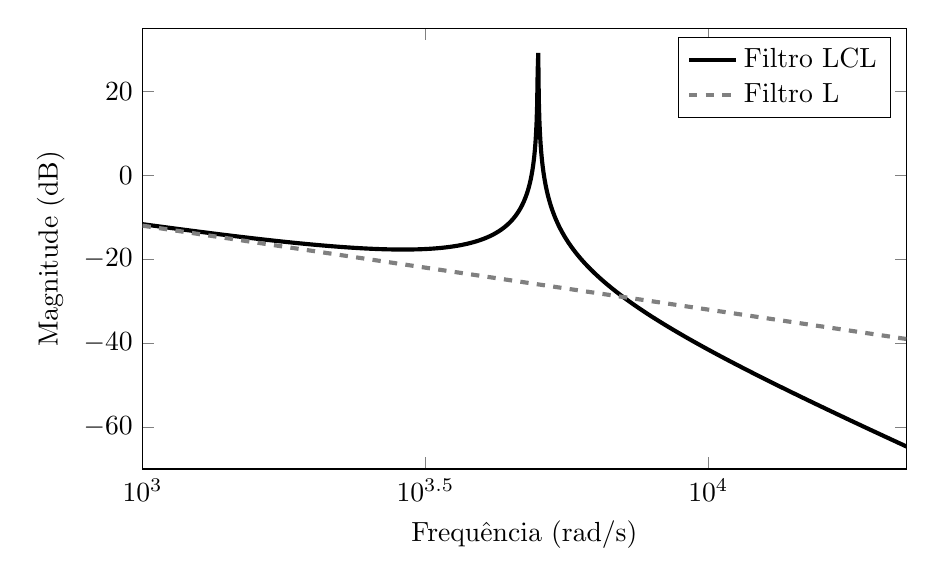
\begin{tikzpicture}

\begin{axis}[%
width=0.8\textwidth,
height=0.461611624834875\textwidth,
scale only axis,
xmode=log,
xmin=1000,
xmax=22387.2113856834,
xtick={1000,3162.27766016838,10000},
xticklabels={{$10^{3}$},{$10^{3.5}$},{$10^{4}$}},
xminorticks=true,
xlabel={Frequência (rad/s)},
ymin=-70,
ymax=35,
ytick={-60, -40, -20,   0,  20},
ylabel={Magnitude (dB)},
legend style={draw=black,fill=white,legend cell align=left}
]
\addplot [color=black,solid,line width=1.5pt]
  table[row sep=crcr]{1000	-11.6866244873506\\
1002.30639260238	-11.7049629837254\\
1004.61810465159	-11.7232934369399\\
1006.93514841637	-11.7416158067243\\
1009.25753619375	-11.7599300525924\\
1011.58528030912	-11.7782361338396\\
1013.9183931163	-11.796534009542\\
1016.2568869976	-11.8148236385551\\
1018.60077436388	-11.8331049795123\\
1020.95006765465	-11.8513779908237\\
1023.30477933808	-11.8696426306744\\
1025.66492191112	-11.8878988570235\\
1028.03050789954	-11.9061466276027\\
1030.40154985798	-11.9243858999147\\
1032.77806037004	-11.9426166312319\\
1035.16005204838	-11.960838778595\\
1037.5475375347	-11.9790522988116\\
1039.94052949988	-11.9972571484547\\
1042.33904064403	-12.0154532838613\\
1044.74308369654	-12.033640661131\\
1047.15267141616	-12.0518192361245\\
1049.56781659108	-12.069988964462\\
1051.98853203896	-12.0881498015219\\
1054.41483060703	-12.1063017024394\\
1056.84672517218	-12.1244446221044\\
1059.28422864096	-12.142578515161\\
1061.72735394972	-12.1607033360049\\
1064.17611406461	-12.1788190387826\\
1066.63052198171	-12.1969255773895\\
1069.09059072708	-12.2150229054686\\
1071.5563333568	-12.2331109764085\\
1074.02776295708	-12.2511897433423\\
1076.50489264432	-12.2692591591457\\
1078.98773556513	-12.2873191764357\\
1081.4763048965	-12.3053697475683\\
1083.97061384575	-12.3234108246377\\
1086.47067565072	-12.3414423594742\\
1088.97650357974	-12.3594643036427\\
1091.48811093176	-12.3774766084408\\
1094.00551103639	-12.3954792248973\\
1096.52871725401	-12.4134721037706\\
1099.05774297578	-12.4314551955469\\
1101.59260162376	-12.4494284504383\\
1104.13330665098	-12.4673918183813\\
1106.67987154147	-12.4853452490351\\
1109.2323098104	-12.5032886917796\\
1111.79063500406	-12.5212220957138\\
1114.35486070002	-12.539145409654\\
1116.92500050717	-12.5570585821319\\
1119.50106806574	-12.5749615613928\\
1122.08307704748	-12.5928542953941\\
1124.67104115564	-12.610736731803\\
1127.26497412507	-12.6286088179948\\
1129.86488972231	-12.6464705010512\\
1132.47080174565	-12.6643217277582\\
1135.0827240252	-12.6821624446044\\
1137.70067042298	-12.6999925977789\\
1140.32465483296	-12.7178121331695\\
1142.95469118117	-12.7356209963606\\
1145.59079342577	-12.7534191326316\\
1148.23297555707	-12.7712064869546\\
1150.8812515977	-12.7889830039923\\
1153.5356356026	-12.8067486280965\\
1156.19614165913	-12.8245033033056\\
1158.86278388715	-12.8422469733428\\
1161.53557643908	-12.8599795816141\\
1164.21453349998	-12.8777010712061\\
1166.89966928762	-12.8954113848838\\
1169.59099805258	-12.913110465089\\
1172.28853407829	-12.9307982539375\\
1174.99229168114	-12.9484746932175\\
1177.70228521052	-12.9661397243874\\
1180.41852904894	-12.9837932885733\\
1183.14103761204	-13.0014353265671\\
1185.86982534876	-13.0190657788243\\
1188.60490674132	-13.0366845854617\\
1191.34629630538	-13.0542916862551\\
1194.09400859005	-13.0718870206373\\
1196.848058178	-13.0894705276956\\
1199.60845968555	-13.1070421461695\\
1202.37522776272	-13.1246018144486\\
1205.14837709331	-13.1421494705702\\
1207.92792239501	-13.1596850522168\\
1210.71387841942	-13.1772084967138\\
1213.5062599522	-13.1947197410275\\
1216.30508181309	-13.212218721762\\
1219.11035885602	-13.2297053751575\\
1221.92210596917	-13.2471796370872\\
1224.74033807505	-13.2646414430555\\
1227.56507013062	-13.2820907281949\\
1230.39631712731	-13.2995274272641\\
1233.23409409112	-13.316951474645\\
1236.07841608273	-13.3343628043403\\
1238.92929819754	-13.3517613499712\\
1241.78675556577	-13.3691470447744\\
1244.65080335254	-13.3865198215997\\
1247.52145675793	-13.4038796129077\\
1250.3987310171	-13.4212263507665\\
1253.28264140034	-13.4385599668496\\
1256.17320321316	-13.4558803924328\\
1259.07043179635	-13.473187558392\\
1261.97434252612	-13.4904813951998\\
1264.88495081411	-13.5077618329234\\
1267.80227210752	-13.5250288012213\\
1270.72632188919	-13.542282229341\\
1273.65711567764	-13.5595220461157\\
1276.5946690272	-13.5767481799617\\
1279.53899752808	-13.5939605588755\\
1282.49011680643	-13.6111591104309\\
1285.44804252445	-13.6283437617763\\
1288.41279038047	-13.6455144396311\\
1291.38437610901	-13.6626710702836\\
1294.36281548089	-13.6798135795874\\
1297.34812430331	-13.6969418929586\\
1300.34031841991	-13.7140559353726\\
1303.33941371088	-13.7311556313613\\
1306.34542609305	-13.74824090501\\
1309.35837151994	-13.7653116799537\\
1312.37826598188	-13.7823678793749\\
1315.40512550606	-13.7994094259996\\
1318.43896615665	-13.8164362420946\\
1321.47980403488	-13.8334482494639\\
1324.52765527909	-13.8504453694458\\
1327.58253606487	-13.8674275229094\\
1330.6444626051	-13.8843946302515\\
1333.71345115004	-13.9013466113927\\
1336.78951798747	-13.9182833857749\\
1339.87267944269	-13.9352048723572\\
1342.96295187868	-13.9521109896126\\
1346.06035169616	-13.969001655525\\
1349.16489533366	-13.985876787585\\
1352.27659926764	-14.0027363027869\\
1355.39548001256	-14.0195801176251\\
1358.52155412096	-14.0364081480903\\
1361.65483818355	-14.0532203096659\\
1364.79534882933	-14.0700165173248\\
1367.94310272563	-14.086796685525\\
1371.09811657822	-14.1035607282066\\
1374.26040713143	-14.1203085587876\\
1377.42999116818	-14.1370400901602\\
1380.6068855101	-14.1537552346873\\
1383.79110701763	-14.1704539041982\\
1386.98267259009	-14.1871360099851\\
1390.18159916578	-14.203801462799\\
1393.38790372205	-14.2204501728457\\
1396.60160327544	-14.2370820497822\\
1399.8227148817	-14.2536970027122\\
1403.05125563594	-14.2702949401822\\
1406.2872426727	-14.2868757701777\\
1409.53069316601	-14.3034394001187\\
1412.78162432955	-14.3199857368559\\
1416.04005341668	-14.3365146866659\\
1419.30599772055	-14.3530261552479\\
1422.5794745742	-14.3695200477184\\
1425.86050135065	-14.3859962686077\\
1429.14909546299	-14.4024547218551\\
1432.44527436445	-14.4188953108047\\
1435.74905554856	-14.4353179382008\\
1439.06045654914	-14.4517225061837\\
1442.3794949405	-14.4681089162849\\
1445.70618833745	-14.4844770694226\\
1449.04055439544	-14.5008268658975\\
1452.38261081064	-14.5171582053874\\
1455.73237532004	-14.5334709869433\\
1459.08986570152	-14.5497651089842\\
1462.45509977397	-14.5660404692925\\
1465.8280953974	-14.582296965009\\
1469.20887047298	-14.5985344926283\\
1472.59744294318	-14.614752947994\\
1475.99383079187	-14.6309522262931\\
1479.39805204436	-14.6471322220519\\
1482.81012476756	-14.6632928291302\\
1486.23006707006	-14.6794339407166\\
1489.65789710218	-14.6955554493234\\
1493.09363305612	-14.7116572467811\\
1496.53729316606	-14.7277392242336\\
1499.9888957082	-14.7438012721324\\
1503.44845900091	-14.7598432802318\\
1506.9160014048	-14.775865137583\\
1510.39154132284	-14.7918667325293\\
1513.87509720044	-14.8078479526998\\
1517.36668752555	-14.8238086850047\\
1520.86633082875	-14.839748815629\\
1524.37404568338	-14.8556682300274\\
1527.88985070559	-14.8715668129182\\
1531.41376455451	-14.8874444482776\\
1534.94580593225	-14.9033010193344\\
1538.4859935841	-14.9191364085632\\
1542.03434629857	-14.9349504976794\\
1545.59088290748	-14.9507431676327\\
1549.15562228612	-14.966514298601\\
1552.72858335329	-14.9822637699848\\
1556.30978507143	-14.9979914604005\\
1559.89924644673	-15.0136972476743\\
1563.49698652918	-15.0293810088363\\
1567.10302441275	-15.0450426201138\\
1570.71737923542	-15.0606819569247\\
1574.34007017931	-15.0762988938716\\
1577.9711164708	-15.0918933047349\\
1581.61053738059	-15.1074650624662\\
1585.25835222385	-15.1230140391818\\
1588.91458036027	-15.1385401061559\\
1592.57924119422	-15.1540431338136\\
1596.25235417481	-15.1695229917245\\
1599.93393879601	-15.1849795485952\\
1603.62401459674	-15.2004126722629\\
1607.322601161	-15.2158222296878\\
1611.02971811795	-15.2312080869462\\
1614.74538514202	-15.2465701092233\\
1618.46962195303	-15.2619081608059\\
1622.20244831628	-15.2772221050749\\
1625.94388404263	-15.2925118044981\\
1629.69394898867	-15.3077771206224\\
1633.45266305675	-15.3230179140666\\
1637.22004619516	-15.3382340445132\\
1640.99611839816	-15.3534253707012\\
1644.78089970617	-15.368591750418\\
1648.57441020578	-15.3837330404913\\
1652.37667002994	-15.3988490967815\\
1656.18769935804	-15.4139397741736\\
1660.00751841599	-15.4290049265685\\
1663.83614747635	-15.4440444068756\\
1667.67360685846	-15.4590580670038\\
1671.51991692849	-15.4740457578534\\
1675.37509809962	-15.4890073293075\\
1679.23917083208	-15.5039426302235\\
1683.11215563331	-15.5188515084243\\
1686.99407305804	-15.5337338106896\\
1690.88494370839	-15.5485893827471\\
1694.78478823403	-15.5634180692633\\
1698.69362733223	-15.578219713835\\
1702.61148174801	-15.5929941589793\\
1706.53837227424	-15.6077412461252\\
1710.47431975172	-15.6224608156038\\
1714.41934506935	-15.6371527066388\\
1718.37346916419	-15.6518167573373\\
1722.33671302159	-15.6664528046799\\
1726.30909767531	-15.6810606845109\\
1730.2906442076	-15.6956402315287\\
1734.28137374936	-15.7101912792757\\
1738.28130748022	-15.7247136601282\\
1742.29046662864	-15.7392072052861\\
1746.30887247206	-15.753671744763\\
1750.33654633699	-15.7681071073754\\
1754.37350959914	-15.7825131207325\\
1758.41978368348	-15.7968896112252\\
1762.47539006444	-15.8112364040157\\
1766.54035026596	-15.8255533230265\\
1770.61468586161	-15.8398401909295\\
1774.69841847474	-15.8540968291347\\
1778.79156977856	-15.8683230577791\\
1782.89416149627	-15.8825186957154\\
1787.00621540116	-15.8966835605004\\
1791.12775331676	-15.9108174683835\\
1795.25879711692	-15.9249202342948\\
1799.39936872594	-15.9389916718336\\
1803.5494901187	-15.953031593256\\
1807.70918332073	-15.9670398094627\\
1811.87847040838	-15.9810161299873\\
1816.05737350894	-15.9949603629833\\
1820.24591480069	-16.0088723152119\\
1824.44411651309	-16.0227517920291\\
1828.65200092687	-16.036598597373\\
1832.86959037413	-16.0504125337506\\
1837.09690723849	-16.064193402225\\
1841.33397395519	-16.0779410024019\\
1845.58081301122	-16.0916551324162\\
1849.83744694544	-16.1053355889183\\
1854.10389834868	-16.1189821670606\\
1858.38018986386	-16.1325946604834\\
1862.66634418617	-16.1461728613008\\
1866.9623840631	-16.1597165600868\\
1871.26833229461	-16.1732255458602\\
1875.58421173328	-16.186699606071\\
1879.91004528435	-16.2001385265848\\
1884.24585590593	-16.2135420916684\\
1888.59166660905	-16.2269100839744\\
1892.94750045783	-16.2402422845263\\
1897.31338056957	-16.2535384727027\\
1901.68933011491	-16.2667984262218\\
1906.0753723179	-16.2800219211257\\
1910.47153045619	-16.2932087317642\\
1914.87782786108	-16.3063586307789\\
1919.29428791772	-16.3194713890864\\
1923.72093406515	-16.3325467758621\\
1928.15778979652	-16.3455845585231\\
1932.60487865912	-16.3585845027116\\
1937.06222425457	-16.3715463722774\\
1941.52985023894	-16.3844699292606\\
1946.00778032282	-16.3973549338738\\
1950.49603827152	-16.4102011444848\\
1954.99464790516	-16.423008317598\\
1959.50363309877	-16.4357762078365\\
1964.02301778248	-16.4485045679232\\
1968.55282594159	-16.4611931486628\\
1973.09308161673	-16.4738416989221\\
1977.64380890397	-16.4864499656111\\
1982.20503195496	-16.499017693664\\
1986.77677497706	-16.5115446260188\\
1991.35906223344	-16.524030503598\\
1995.95191804325	-16.5364750652881\\
2000.55536678172	-16.5488780479194\\
2005.16943288031	-16.5612391862453\\
2009.79414082682	-16.5735582129212\\
2014.42951516552	-16.5858348584837\\
2019.07558049731	-16.5980688513288\\
2023.73236147981	-16.6102599176902\\
2028.39988282751	-16.6224077816176\\
2033.07816931193	-16.6345121649542\\
2037.76724576168	-16.646572787314\\
2042.46713706267	-16.6585893660593\\
2047.17786815819	-16.6705616162774\\
2051.89946404906	-16.682489250757\\
2056.63194979376	-16.6943719799646\\
2061.37535050858	-16.7062095120206\\
2066.12969136771	-16.7180015526747\\
2070.89499760343	-16.7297478052811\\
2075.6712945062	-16.741447970774\\
2080.45860742482	-16.7531017476417\\
2085.25696176653	-16.7647088319015\\
2090.0663829972	-16.7762689170732\\
2094.88689664142	-16.7877816941529\\
2099.71852828265	-16.7992468515865\\
2104.56130356336	-16.8106640752426\\
2109.41524818514	-16.8220330483847\\
2114.2803879089	-16.8333534516442\\
2119.15674855492	-16.8446249629915\\
2124.04435600306	-16.8558472577078\\
2128.94323619287	-16.8670200083563\\
2133.8534151237	-16.8781428847529\\
2138.7749188549	-16.8892155539361\\
2143.70777350589	-16.9002376801376\\
2148.65200525637	-16.9112089247512\\
2153.60764034637	-16.9221289463021\\
2158.57470507649	-16.9329974004158\\
2163.55322580795	-16.943813939786\\
2168.5432289628	-16.9545782141424\\
2173.54474102401	-16.9652898702184\\
2178.55778853565	-16.9759485517176\\
2183.58239810298	-16.9865538992806\\
2188.61859639264	-16.9971055504506\\
2193.66641013278	-17.0076031396394\\
2198.7258661132	-17.0180462980919\\
2203.79699118545	-17.028434653851\\
2208.87981226306	-17.0387678317215\\
2213.97435632161	-17.0490454532336\\
2219.08065039887	-17.0592671366059\\
2224.19872159503	-17.0694324967081\\
2229.32859707273	-17.0795411450229\\
2234.47030405729	-17.0895926896069\\
2239.6238698368	-17.0995867350523\\
2244.78932176229	-17.1095228824466\\
2249.9666872479	-17.1194007293326\\
2255.15599377096	-17.1292198696673\\
2260.3572688722	-17.1389798937809\\
2265.57054015585	-17.1486803883343\\
2270.79583528983	-17.1583209362767\\
2276.03318200585	-17.1679011168022\\
2281.28260809959	-17.177420505306\\
2286.54414143084	-17.1868786733398\\
2291.81780992365	-17.1962751885667\\
2297.10364156645	-17.205609614715\\
2302.40166441225	-17.2148815115321\\
2307.71190657875	-17.2240904347368\\
2313.0343962485	-17.2332359359717\\
2318.36916166905	-17.2423175627545\\
2323.7162311531	-17.2513348584282\\
2329.07563307865	-17.2602873621116\\
2334.44739588916	-17.2691746086479\\
2339.83154809368	-17.2779961285533\\
2345.22811826701	-17.2867514479643\\
2350.63713504986	-17.2954400885848\\
2356.05862714902	-17.3040615676319\\
2361.49262333744	-17.3126153977807\\
2366.93915245447	-17.3211010871091\\
2372.39824340596	-17.329518139041\\
2377.86992516445	-17.3378660522885\\
2383.35422676926	-17.3461443207941\\
2388.85117732672	-17.3543524336712\\
2394.36080601029	-17.3624898751438\\
2399.88314206069	-17.3705561244854\\
2405.4182147861	-17.3785506559571\\
2410.96605356231	-17.3864729387445\\
2416.52668783283	-17.3943224368935\\
2422.10014710909	-17.4020986092452\\
2427.6864609706	-17.40980090937\\
2433.28565906507	-17.4174287855003\\
2438.8977711086	-17.4249816804623\\
2444.52282688584	-17.4324590316065\\
2450.16085625011	-17.4398602707377\\
2455.8118891236	-17.4471848240427\\
2461.4759554975	-17.4544321120183\\
2467.15308543219	-17.4616015493969\\
2472.84330905736	-17.4686925450715\\
2478.54665657221	-17.4757045020194\\
2484.26315824557	-17.4826368172242\\
2489.9928444161	-17.4894888815976\\
2495.73574549243	-17.4962600798985\\
2501.49189195332	-17.5029497906518\\
2507.26131434783	-17.5095573860656\\
2513.04404329547	-17.5160822319466\\
2518.84010948637	-17.5225236876147\\
2524.64954368146	-17.5288811058156\\
2530.4723767126	-17.5351538326325\\
2536.30863948277	-17.5413412073959\\
2542.15836296621	-17.5474425625916\\
2548.02157820863	-17.5534572237683\\
2553.8983163273	-17.5593845094418\\
2559.7886085113	-17.5652237309995\\
2565.69248602162	-17.5709741926019\\
2571.60998019135	-17.5766351910827\\
2577.54112242586	-17.5822060158477\\
2583.48594420295	-17.587685948771\\
2589.444477073	-17.5930742640905\\
2595.41675265919	-17.5983702283007\\
2601.4028026576	-17.6035731000439\\
2607.40265883745	-17.6086821299994\\
2613.41635304121	-17.6136965607711\\
2619.4439171848	-17.6186156267727\\
2625.48538325773	-17.6234385541108\\
2631.54078332332	-17.6281645604665\\
2637.61014951883	-17.632792854974\\
2643.69351405564	-17.6373226380976\\
2649.7909092194	-17.6417531015068\\
2655.90236737027	-17.646083427948\\
2662.02792094301	-17.6503127911149\\
2668.16760244719	-17.6544403555161\\
2674.32144446738	-17.6584652763404\\
2680.48947966327	-17.6623866993194\\
2686.67174076992	-17.6662037605881\\
2692.86826059784	-17.6699155865418\\
2699.07907203326	-17.6735212936917\\
2705.30420803822	-17.6770199885171\\
2711.54370165082	-17.6804107673144\\
2717.79758598533	-17.6836927160443\\
2724.0658942324	-17.6868649101751\\
2730.34865965925	-17.6899264145239\\
2736.64591560979	-17.6928762830938\\
2742.95769550488	-17.6957135589089\\
2749.28403284242	-17.6984372738459\\
2755.6249611976	-17.7010464484617\\
2761.98051422303	-17.7035400918189\\
2768.35072564895	-17.7059172013068\\
2774.73562928336	-17.7081767624598\\
2781.13525901229	-17.7103177487714\\
2787.54964879989	-17.7123391215052\\
2793.97883268864	-17.714239829502\\
2800.42284479955	-17.7160188089828\\
2806.88171933232	-17.7176749833482\\
2813.35549056553	-17.7192072629737\\
2819.84419285683	-17.7206145450008\\
2826.34786064309	-17.721895713124\\
2832.86652844062	-17.7230496373734\\
2839.40023084533	-17.7240751738932\\
2845.94900253294	-17.7249711647149\\
2852.51287825912	-17.7257364375268\\
2859.09189285972	-17.7263698054385\\
2865.68608125093	-17.7268700667396\\
2872.29547842946	-17.7272360046551\\
2878.92011947275	-17.7274663870942\\
2885.56003953913	-17.7275599663946\\
2892.21527386804	-17.7275154790612\\
2898.88585778017	-17.7273316454995\\
2905.57182667768	-17.7270071697432\\
2912.27321604441	-17.7265407391757\\
2918.99006144599	-17.7259310242465\\
2925.72239853012	-17.7251766781805\\
2932.4702630267	-17.7242763366819\\
2939.23369074803	-17.7232286176312\\
2946.01271758903	-17.7220321207754\\
2952.80737952738	-17.7206854274125\\
2959.61771262377	-17.7191871000678\\
2966.44375302203	-17.7175356821638\\
2973.28553694936	-17.7157296976828\\
2980.14310071653	-17.7137676508218\\
2987.01648071805	-17.7116480256393\\
2993.90571343235	-17.7093692856956\\
3000.81083542203	-17.7069298736832\\
3007.73188333397	-17.7043282110499\\
3014.66889389963	-17.7015626976135\\
3021.62190393513	-17.6986317111669\\
3028.59095034155	-17.6955336070749\\
3035.57607010504	-17.6922667178612\\
3042.57730029708	-17.6888293527862\\
3049.59467807464	-17.6852197974147\\
3056.6282406804	-17.6814363131738\\
3063.67802544292	-17.6774771369003\\
3070.74406977686	-17.6733404803774\\
3077.82641118319	-17.66902452986\\
3084.92508724934	-17.6645274455901\\
3092.04013564946	-17.6598473612986\\
3099.17159414457	-17.6549823836971\\
3106.3195005828	-17.6499305919559\\
3113.48389289956	-17.6446900371703\\
3120.66480911777	-17.6392587418133\\
3127.86228734801	-17.6336346991756\\
3135.0763657888	-17.6278158727909\\
3142.30708272674	-17.6218001958477\\
3149.55447653674	-17.6155855705862\\
3156.8185856822	-17.6091698676802\\
3164.09944871527	-17.6025509256033\\
3171.39710427697	-17.5957265499794\\
3178.71159109747	-17.5886945129167\\
3186.04294799627	-17.5814525523243\\
3193.39121388238	-17.5739983712118\\
3200.75642775457	-17.5663296369705\\
3208.13862870155	-17.5584439806365\\
3215.53785590219	-17.5503389961338\\
3222.9541486257	-17.5420122394984\\
3230.38754623189	-17.5334612280815\\
3237.83808817133	-17.5246834397318\\
3245.30581398558	-17.5156763119564\\
3252.79076330741	-17.5064372410583\\
3260.29297586098	-17.4969635812521\\
3267.81249146208	-17.4872526437546\\
3275.34935001834	-17.4773016958512\\
3282.90359152942	-17.4671079599374\\
3290.47525608724	-17.4566686125325\\
3298.06438387618	-17.4459807832677\\
3305.67101517332	-17.435041553845\\
3313.2951903486	-17.4238479569678\\
3320.93694986511	-17.4123969752406\\
3328.59633427924	-17.4006855400384\\
3336.27338424092	-17.3887105303439\\
3343.96814049384	-17.3764687715511\\
3351.68064387566	-17.363957034235\\
3359.41093531822	-17.3511720328854\\
3367.15905584778	-17.3381104246041\\
3374.92504658521	-17.3247688077641\\
3382.70894874623	-17.3111437206293\\
3390.51080364161	-17.2972316399335\\
3398.3306526774	-17.2830289794168\\
3406.16853735517	-17.2685320883185\\
3414.02449927217	-17.2537372498249\\
3421.89858012163	-17.2386406794695\\
3429.7908216929	-17.2232385234846\\
3437.70126587175	-17.2075268571033\\
3445.62995464054	-17.1915016828072\\
3453.57693007845	-17.175158928522\\
3461.54223436172	-17.1584944457549\\
3469.52590976386	-17.1415040076746\\
3477.5279986559	-17.1241833071301\\
3485.54854350656	-17.1065279546063\\
3493.58758688252	-17.0885334761148\\
3501.64517144866	-17.0701953110162\\
3509.72133996824	-17.0515088097714\\
3517.81613530314	-17.0324692316206\\
3525.92960041413	-17.0130717421849\\
3534.06177836102	-16.9933114109889\\
3542.21271230298	-16.9731832089013\\
3550.38244549868	-16.9526820054888\\
3558.57102130658	-16.9318025662813\\
3566.77848318515	-16.910539549944\\
3575.00487469309	-16.8888875053527\\
3583.25023948954	-16.8668408685683\\
3591.51462133436	-16.8443939597065\\
3599.79806408833	-16.8215409796978\\
3608.10061171339	-16.7982760069338\\
3616.42230827288	-16.7745929937949\\
3624.76319793175	-16.7504857630533\\
3633.12332495683	-16.7259480041476\\
3641.50273371703	-16.7009732693221\\
3649.90146868361	-16.675554969625\\
3658.31957443038	-16.6496863707608\\
3666.75709563398	-16.6233605887873\\
3675.21407707406	-16.5965705856544\\
3683.69056363357	-16.5693091645735\\
3692.18660029898	-16.5415689652125\\
3700.7022321605	-16.5133424587075\\
3709.23750441235	-16.4846219424831\\
3717.79246235299	-16.455399534871\\
3726.36715138533	-16.4256671695201\\
3734.96161701703	-16.3954165895856\\
3743.57590486067	-16.3646393416884\\
3752.21006063408	-16.3333267696324\\
3760.86413016048	-16.3014700078695\\
3769.53815936883	-16.2690599746986\\
3778.23219429398	-16.2360873651865\\
3786.94628107696	-16.2025426437964\\
3795.68046596523	-16.1684160367095\\
3804.43479531292	-16.1336975238244\\
3813.20931558105	-16.0983768304179\\
3822.00407333782	-16.0624434184495\\
3830.81911525882	-16.0258864774918\\
3839.65448812729	-15.9886949152667\\
3848.51023883439	-15.9508573477672\\
3857.38641437941	-15.9123620889424\\
3866.28306187004	-15.8731971399223\\
3875.20022852263	-15.8333501777583\\
3884.13796166242	-15.7928085436517\\
3893.09630872381	-15.7515592306438\\
3902.07531725059	-15.7095888707352\\
3911.07503489621	-15.6668837214059\\
3920.09550942403	-15.6234296514981\\
3929.13678870758	-15.579212126429\\
3938.19892073078	-15.534216192693\\
3947.28195358824	-15.4884264616122\\
3956.38593548549	-15.4418270922917\\
3965.51091473924	-15.3944017737315\\
3974.65693977764	-15.3461337060458\\
3983.82405914052	-15.2970055807341\\
3993.0123214797	-15.2469995599475\\
4002.22177555915	-15.1960972546871\\
4011.45247025537	-15.1442797018684\\
4020.70445455755	-15.0915273401806\\
4029.97777756789	-15.0378199846622\\
4039.27248850181	-14.9831367999125\\
4048.58863668828	-14.9274562718486\\
4057.92627157	-14.8707561779121\\
4067.28544270374	-14.8130135556239\\
4076.66619976054	-14.7542046693734\\
4086.06859252603	-14.694304975324\\
4095.49267090063	-14.633289084304\\
4104.93848489989	-14.5711307225432\\
4114.40608465467	-14.5078026901027\\
4123.89552041149	-14.4432768168335\\
4133.40684253274	-14.3775239156862\\
4142.94010149697	-14.3105137331772\\
4152.49534789915	-14.2422148968023\\
4162.07263245095	-14.1725948591669\\
4171.67200598098	-14.1016198385874\\
4181.29351943512	-14.0292547558883\\
4190.93722387671	-13.9554631671028\\
4200.60317048688	-13.8802071917523\\
4210.29141056481	-13.803447436351\\
4220.00199552799	-13.7251429127506\\
4229.73497691249	-13.6452509509009\\
4239.49040637325	-13.5637271055607\\
4249.26833568435	-13.480525056451\\
4259.06881673929	-13.3955965012869\\
4268.89190155123	-13.3088910410707\\
4278.73764225331	-13.220356056966\\
4288.60609109892	-13.129936577997\\
4298.49730046193	-13.0375751387441\\
4308.41132283705	-12.9432116261104\\
4318.34821084004	-12.8467831141389\\
4328.30801720801	-12.7482236857429\\
4338.2907947997	-12.6474642400869\\
4348.29659659578	-12.5444322842063\\
4358.32547569911	-12.4390517072965\\
4368.37748533501	-12.3312425359094\\
4378.45267885158	-12.2209206680866\\
4388.55110971994	-12.1079975842178\\
4398.67283153454	-11.9923800321336\\
4408.81789801347	-11.8739696836287\\
4418.98636299867	-11.7526627592474\\
4429.17828045629	-11.6283496177462\\
4439.39370447695	-11.5009143061649\\
4449.63268927599	-11.3702340658847\\
4459.89528919383	-11.2361787893997\\
4470.1815586962	-11.0986104217832\\
4480.49155237445	-10.95738229995\\
4490.82532494586	-10.8123384217914\\
4501.18293125388	-10.6633126360597\\
4511.56442626847	-10.5101277424578\\
4521.96986508636	-10.3525944897218\\
4532.39930293136	-10.1905104574974\\
4542.85279515466	-10.0236588054516\\
4553.33039723509	-9.85180687024205\\
4563.83216477945	-9.67470458758291\\
4574.35815352278	-9.49208271257272\\
4584.90841932869	-9.30365080651984\\
4595.4830181896	-9.10909495250763\\
4606.0820062271	-8.90807515462322\\
4616.7054396922	-8.70022236678049\\
4627.35337496566	-8.4851350859756\\
4638.02586855826	-8.26237543102767\\
4648.72297711113	-8.03146461064706\\
4659.44475739604	-7.79187766302813\\
4670.19126631568	-7.543037321771\\
4680.96256090399	-7.28430682800527\\
4691.75869832646	-7.0149814637226\\
4702.57973588042	-6.73427852319908\\
4713.42573099534	-6.44132536345532\\
4724.29674123316	-6.13514507455255\\
4735.19282428857	-5.81463917712859\\
4746.11403798933	-5.47856657495979\\
4757.06044029659	-5.12551774568802\\
4768.03208930514	-4.75388281538841\\
4779.02904324381	-4.36181169081674\\
4790.05136047569	-3.94716375357916\\
4801.09909949849	-3.50744365468524\\
4812.17231894485	-3.0397183299378\\
4823.27107758263	-2.54050823324241\\
4834.39543431522	-2.00564253513636\\
4845.54544818189	-1.43006293738706\\
4856.72117835806	-0.807552539966115\\
4867.92268415562	-0.130352538873392\\
4879.1500250233	0.61139399502118\\
4890.4032605469	1.43047423386148\\
4901.68245044966	2.34389609488669\\
4912.98765459258	3.37497808039193\\
4924.31893297469	4.55691770362268\\
4935.67634573345	5.93930398182023\\
4947.05995314498	7.60107573753444\\
4958.46981562442	9.6795174594279\\
4969.90599372628	12.4472154543316\\
4981.36854814472	16.5818910560937\\
4992.85753971387	24.8798662484055\\
5004.37302940819	29.111161356491\\
5015.91507834275	17.8606085563392\\
5027.48374777359	13.0852284200695\\
5039.07909909802	9.99780844818535\\
5050.70119385497	7.70627588230236\\
5062.35009372529	5.8798261437457\\
5074.02586053209	4.3588162994333\\
5085.72855624109	3.05388110822874\\
5097.45824296091	1.90991394525242\\
5109.21498294339	0.890523712176367\\
5120.998838584	-0.02958473491872\\
5132.80987242209	-0.868708271507068\\
5144.64814714125	-1.6405104838289\\
5156.51372556965	-2.35546499573745\\
5168.40667068035	-3.02177716025602\\
5180.32704559168	-3.64599517449879\\
5192.27491356753	-4.23342831113557\\
5204.25033801768	-4.78844100331898\\
5216.2533824982	-5.31466453723398\\
5228.28411071172	-5.81515258877364\\
5240.34258650779	-6.29249758312595\\
5252.42887388322	-6.7489191531472\\
5264.54303698246	-7.18633235878933\\
5276.68514009784	-7.6064009819906\\
5288.85524767004	-8.01057965142835\\
5301.0534242883	-8.40014749385769\\
5313.27973469088	-8.77623527850186\\
5325.53424376533	-9.13984750829142\\
5337.81701654885	-9.4918805463744\\
5350.12811822866	-9.83313760225341\\
5362.46761414231	-10.1643412086219\\
5374.83556977805	-10.4861436767945\\
5387.23205077517	-10.7991359114227\\
5399.65712292437	-11.1038548840794\\
5412.11085216805	-11.4007900033553\\
5424.59330460073	-11.6903885713931\\
5437.10454646936	-11.973060479706\\
5449.64464417369	-12.2491822680986\\
5462.21366426659	-12.5191006476222\\
5474.81167345445	-12.7831355703073\\
5487.43873859751	-13.0415829138903\\
5500.09492671021	-13.2947168380652\\
5512.78030496154	-13.5427918593358\\
5525.49494067543	-13.7860446838583\\
5538.23890133107	-14.0246958313764\\
5551.0122545633	-14.2589510781876\\
5563.81506816292	-14.4890027428124\\
5576.64741007712	-14.7150308345075\\
5589.50934840979	-14.9372040818116\\
5602.40095142188	-15.1556808558563\\
5615.32228753178	-15.3706100011037\\
5628.2734253157	-15.5821315844288\\
5641.254433508	-15.7903775719936\\
5654.26538100157	-15.9954724421079\\
5667.30633684818	-16.1975337412059\\
5680.37737025889	-16.3966725891601\\
5693.47855060436	-16.592994139373\\
5706.60994741527	-16.7865979984179\\
5719.77163038263	-16.9775786094222\\
5732.96366935823	-17.1660256028898\\
5746.18613435493	-17.3520241182248\\
5759.43909554709	-17.5356550988454\\
5772.72262327089	-17.7169955634481\\
5786.03678802477	-17.8961188556993\\
5799.38166046975	-18.0730948743803\\
5812.75731142982	-18.2479902857937\\
5826.16381189231	-18.4208687200473\\
5839.60123300829	-18.5917909526613\\
5853.06964609293	-18.7608150727975\\
5866.56912262587	-18.9279966392752\\
5880.09973425162	-19.0933888254217\\
5893.66155277994	-19.2570425537053\\
5907.25465018618	-19.419006621001\\
5920.87909861173	-19.5793278152613\\
5934.53497036433	-19.7380510242914\\
5948.22233791852	-19.8952193372587\\
5961.94127391598	-20.0508741395145\\
5975.69185116595	-20.2050552012468\\
5989.47414264556	-20.357800760442\\
6003.28822150028	-20.5091476005869\\
6017.13416104428	-20.6591311235069\\
6031.01203476082	-20.8077854177005\\
6044.92191630263	-20.955143322501\\
6058.86387949234	-21.1012364883672\\
6072.83799832281	-21.2460954335796\\
6086.84434695757	-21.3897495975965\\
6100.88299973121	-21.5322273913045\\
6114.95403114975	-21.6735562443749\\
6129.05751589107	-21.8137626499274\\
6143.19352880526	-21.95287220668\\
6157.36214491506	-22.0909096587544\\
6171.56343941624	-22.2278989332906\\
6185.79748767801	-22.3638631760156\\
6200.06436524339	-22.4988247848959\\
6214.36414782964	-22.6328054419986\\
6228.69691132868	-22.7658261436727\\
6243.06273180741	-22.8979072291567\\
6257.46168550822	-23.0290684077097\\
6271.89384884933	-23.1593287843565\\
6286.3592984252	-23.2887068843304\\
6300.85811100697	-23.417220676293\\
6315.39036354283	-23.5448875944023\\
6329.95613315842	-23.6717245592983\\
6344.5554971573	-23.7977479980685\\
6359.18853302131	-23.9229738632523\\
6373.85531841099	-24.0474176509391\\
6388.55593116599	-24.1710944180124\\
6403.2904493055	-24.294018798586\\
6418.05895102865	-24.41620501968\\
6432.86151471491	-24.5376669161752\\
6447.69821892457	-24.6584179450884\\
6462.56914239904	-24.7784711992027\\
6477.47436406142	-24.8978394200898\\
6492.41396301678	-25.0165350105545\\
6507.38801855265	-25.1345700465335\\
6522.39661013943	-25.2519562884755\\
6537.43981743082	-25.3687051922316\\
6552.51772026422	-25.4848279194778\\
6567.63039866118	-25.6003353476976\\
6582.7779328278	-25.7152380797431\\
6597.96040315516	-25.8295464529979\\
6613.17789021976	-25.9432705481611\\
6628.43047478397	-26.0564201976709\\
6643.71823779637	-26.1690049937849\\
6659.0412603923	-26.2810342963352\\
6674.39962389419	-26.3925172401719\\
6689.79340981204	-26.5034627423121\\
6705.22269984386	-26.6138795088061\\
6720.68757587607	-26.7237760413358\\
6736.18811998395	-26.8331606435569\\
6751.7244144321	-26.9420414271968\\
6767.29654167483	-27.0504263179199\\
6782.90458435663	-27.15832306097\\
6798.54862531262	-27.2657392266011\\
6814.22874756894	-27.3726822153043\\
6829.94503434323	-27.4791592628423\\
6845.69756904508	-27.5851774450974\\
6861.48643527643	-27.6907436827434\\
6877.31171683206	-27.7958647457468\\
6893.1734977	-27.9005472577079\\
6909.07186206198	-28.0047977000445\\
6925.00689429393	-28.108622416029\\
6940.97867896634	-28.2120276146817\\
6956.98730084476	-28.3150193745291\\
6973.03284489025	-28.417603647231\\
6989.11539625984	-28.5197862610823\\
7005.23504030692	-28.6215729243949\\
7021.3918625818	-28.7229692287649\\
7037.58594883204	-28.8239806522285\\
7053.81738500302	-28.9246125623128\\
7070.0862572383	-29.0248702189841\\
7086.39265188016	-29.124758777499\\
7102.73665546999	-29.2242832911612\\
7119.11835474879	-29.3234487139886\\
7135.53783665763	-29.4222599032934\\
7151.99518833808	-29.5207216221791\\
7168.49049713269	-29.618838541957\\
7185.02385058548	-29.7166152444867\\
7201.59533644237	-29.8140562244408\\
7218.20504265165	-29.9111658915004\\
7234.85305736446	-30.0079485724799\\
7251.53946893525	-30.1044085133873\\
7268.26436592224	-30.2005498814199\\
7285.02783708792	-30.2963767668997\\
7301.82997139948	-30.3918931851483\\
7318.67085802933	-30.4871030783066\\
7335.55058635552	-30.5820103170984\\
7352.46924596225	-30.6766187025418\\
7369.42692664033	-30.7709319676094\\
7386.42371838769	-30.8649537788394\\
7403.45971140979	-30.9586877378993\\
7420.53499612018	-31.0521373831039\\
7437.64966314091	-31.1453061908888\\
7454.80380330304	-31.2381975772418\\
7471.99750764715	-31.3308148990929\\
7489.23086742376	-31.4231614556644\\
7506.50397409388	-31.515240489783\\
7523.81691932944	-31.6070551891541\\
7541.16979501382	-31.6986086876014\\
7558.56269324229	-31.7899040662708\\
7575.99570632259	-31.8809443548015\\
7593.46892677529	-31.9717325324641\\
7610.98244733438	-32.0622715292681\\
7628.53636094773	-32.152564227039\\
7646.13076077758	-32.2426134604655\\
7663.76574020103	-32.3324220181189\\
7681.44139281058	-32.4219926434455\\
7699.15781241454	-32.511328035731\\
7716.91509303763	-32.6004308510411\\
7734.71332892138	-32.6893037031358\\
7752.55261452471	-32.7779491643602\\
7770.43304452438	-32.8663697665117\\
7788.35471381553	-32.9545680016853\\
7806.31771751215	-33.0425463230957\\
7824.32215094763	-33.1303071458796\\
7842.36810967519	-33.2178528478766\\
7860.45568946846	-33.3051857703902\\
7878.58498632195	-33.3923082189297\\
7896.7560964516	-33.4792224639334\\
7914.96911629522	-33.5659307414732\\
7933.22414251308	-33.6524352539424\\
7951.52127198837	-33.7387381707253\\
7969.86060182773	-33.8248416288509\\
7988.24222936175	-33.9107477336308\\
8006.66625214554	-33.9964585592805\\
8025.13276795918	-34.0819761495261\\
8043.6418748083	-34.1673025181967\\
8062.19367092452	-34.2524396498015\\
8080.78825476607	-34.3373895000937\\
8099.42572501823	-34.4221539966207\\
8118.10618059391	-34.5067350392615\\
8136.82972063413	-34.5911345007506\\
8155.5964445086	-34.6753542271906\\
8174.40645181619	-34.7593960385517\\
8193.25984238548	-34.8432617291601\\
8212.1567162753	-34.9269530681753\\
8231.09717377527	-35.0104718000555\\
8250.08131540631	-35.0938196450132\\
8269.10924192116	-35.1769982994597\\
8288.18105430498	-35.2600094364396\\
8307.29685377578	-35.3428547060555\\
8326.45674178507	-35.4255357358834\\
8345.66082001834	-35.508054131378\\
8364.90919039556	-35.5904114762693\\
8384.20195507185	-35.672609332951\\
8403.53921643786	-35.7546492428587\\
8422.92107712042	-35.8365327268414\\
8442.3476399831	-35.9182612855237\\
8461.81900812665	-35.9998363996605\\
8481.33528488963	-36.0812595304839\\
8500.89657384898	-36.1625321200428\\
8520.50297882047	-36.2436555915343\\
8540.15460385935	-36.3246313496289\\
8559.85155326084	-36.4054607807887\\
8579.59393156072	-36.4861452535775\\
8599.38184353586	-36.5666861189664\\
8619.21539420481	-36.6470847106309\\
8639.09468882829	-36.7273423452431\\
8659.01983290983	-36.8074603227569\\
8678.99093219629	-36.887439926688\\
8699.00809267839	-36.9672824243874\\
8719.07142059136	-37.0469890673097\\
8739.18102241541	-37.1265610912753\\
8759.33700487634	-37.205999716728\\
8779.5394749461	-37.2853061489864\\
8799.78853984339	-37.3644815784912\\
8820.08430703416	-37.4435271810462\\
8840.42688423224	-37.522444118056\\
8860.81637939989	-37.6012335367571\\
8881.25290074835	-37.6798965704461\\
8901.73655673847	-37.7584343387019\\
8922.26745608124	-37.8368479476049\\
8942.84570773836	-37.9151384899501\\
8963.47142092288	-37.9933070454575\\
8984.14470509972	-38.0713546809779\\
9004.86566998624	-38.1492824506942\\
9025.63442555289	-38.2270913963194\\
9046.45108202374	-38.3047825472903\\
9067.31574987707	-38.3823569209579\\
9088.228539846	-38.4598155227734\\
9109.18956291901	-38.5371593464717\\
9130.19893034058	-38.6143893742502\\
9151.25675361173	-38.6915065769448\\
9172.36314449071	-38.7685119142029\\
9193.51821499347	-38.8454063346525\\
9214.72207739435	-38.9221907760681\\
9235.97484422661	-38.9988661655341\\
9257.27662828307	-39.0754334196046\\
9278.62754261669	-39.15189344446\\
9300.02770054119	-39.228247136062\\
9321.47721563161	-39.3044953803037\\
9342.97620172496	-39.3806390531588\\
9364.5247729208	-39.456679020827\\
9386.12304358183	-39.5326161398768\\
9407.77112833455	-39.6084512573864\\
9429.46914206979	-39.6841852110812\\
9451.21719994339	-39.7598188294692\\
9473.0154173768	-39.835352931974\\
9494.86391005764	-39.9107883290655\\
9516.76279394036	-39.9861258223874\\
9538.71218524688	-40.0613662048841\\
9560.71220046713	-40.1365102609234\\
9582.76295635973	-40.2115587664186\\
9604.86456995261	-40.2865124889477\\
9627.01715854358	-40.3613721878704\\
9649.22083970099	-40.4361386144433\\
9671.47573126437	-40.5108125119334\\
9693.78195134502	-40.5853946157289\\
9716.13961832666	-40.6598856534486\\
9738.54885086602	-40.7342863450492\\
9761.00976789355	-40.8085974029308\\
9783.52248861393	-40.8828195320407\\
9806.08713250686	-40.9569534299755\\
9828.70381932752	-41.0309997870806\\
9851.37266910737	-41.1049592865494\\
9874.09380215466	-41.1788326045199\\
9896.86733905512	-41.2526204101697\\
9919.69340067262	-41.3263233658097\\
9942.57210814977	-41.3999421269761\\
9965.5035829086	-41.4734773425209\\
9988.48794665118	-41.5469296547009\\
10011.5253213603	-41.620299699265\\
10034.6158293	-41.6935881055404\\
10057.7595930163	-41.7667954965171\\
10080.9567353382	-41.8399224889312\\
10104.2073793774	-41.9129696933469\\
10127.5116485301	-41.9859377142369\\
10150.8696664767	-42.0588271500612\\
10174.2815571832	-42.131638593346\\
10197.7474449012	-42.2043726307592\\
10221.267454169	-42.277029843187\\
10244.8417098122	-42.349610805807\\
10268.4703369442	-42.4221160881623\\
10292.1534609671	-42.4945462542325\\
10315.891207572	-42.5669018625049\\
10339.68370274	-42.6391834660438\\
10363.5310727429	-42.7113916125594\\
10387.4334441436	-42.783526844475\\
10411.3909437969	-42.8555896989931\\
10435.4036988501	-42.9275807081612\\
10459.4718367439	-42.9995003989359\\
10483.5954852129	-43.0713492932459\\
10507.7747722864	-43.1431279080549\\
10532.0098262886	-43.2148367554226\\
10556.3007758401	-43.2864763425651\\
10580.647749858	-43.3580471719144\\
10605.0508775566	-43.4295497411771\\
10629.5102884484	-43.500984543392\\
10654.0261123446	-43.5723520669868\\
10678.5984793556	-43.6436527958342\\
10703.2275198921	-43.7148872093069\\
10727.9133646656	-43.7860557823319\\
10752.6561446888	-43.8571589854438\\
10777.4559912768	-43.9281972848375\\
10802.3130360475	-43.9991711424204\\
10827.2274109224	-44.0700810158629\\
10852.1992481272	-44.140927358649\\
10877.2286801926	-44.2117106201259\\
10902.315839955	-44.282431245553\\
10927.460860557	-44.3530896761495\\
10952.6638754485	-44.4236863491423\\
10977.9250183872	-44.4942216978126\\
11003.244423439	-44.564696151542\\
11028.6222249794	-44.6351101358575\\
11054.0585576935	-44.7054640724765\\
11079.5535565772	-44.7757583793511\\
11105.1073569377	-44.8459934707111\\
11130.7200943943	-44.916169757107\\
11156.3919048792	-44.986287645452\\
11182.1229246378	-45.0563475390639\\
11207.9132902301	-45.1263498377059\\
11233.7631385307	-45.1962949376271\\
11259.6726067303	-45.266183231602\\
11285.6418323356	-45.3360151089705\\
11311.6709531708	-45.4057909556756\\
11337.7601073777	-45.4755111543027\\
11363.9094334169	-45.5451760841161\\
11390.1190700682	-45.6147861210971\\
11416.3891564316	-45.6843416379801\\
11442.7198319278	-45.7538430042886\\
11469.1112362992	-45.823290586371\\
11495.5635096105	-45.8926847474356\\
11522.0767922492	-45.9620258475855\\
11548.6512249268	-46.031314243852\\
11575.2869486794	-46.1005502902293\\
11601.9841048683	-46.1697343377066\\
11628.7428351806	-46.2388667343019\\
11655.5632816306	-46.3079478250934\\
11682.4455865599	-46.3769779522518\\
11709.3898926384	-46.4459574550721\\
11736.3963428651	-46.5148866700039\\
11763.4650805689	-46.5837659306822\\
11790.596249409	-46.6525955679581\\
11817.7899933763	-46.7213759099278\\
11845.0464567934	-46.7901072819625\\
11872.3657843162	-46.8587900067374\\
11899.7481209338	-46.9274244042601\\
11927.1936119701	-46.9960107918988\\
11954.7024030838	-47.0645494844104\\
11982.2746402699	-47.1330407939677\\
12009.9104698599	-47.2014850301868\\
12037.6100385228	-47.2698825001539\\
12065.3734932659	-47.3382335084512\\
12093.2009814357	-47.4065383571837\\
12121.0926507183	-47.4747973460045\\
12149.0486491407	-47.5430107721403\\
12177.069125071	-47.6111789304165\\
12205.1542272196	-47.6793021132819\\
12233.3041046402	-47.7473806108334\\
12261.5189067297	-47.8154147108399\\
12289.7987832301	-47.8834046987658\\
12318.1438842284	-47.9513508577951\\
12346.554360158	-48.0192534688546\\
12375.0303617991	-48.0871128106361\\
12403.5720402798	-48.15492915962\\
12432.1795470765	-48.2227027900968\\
12460.8530340153	-48.2904339741896\\
12489.5926532723	-48.358122981876\\
12518.3985573745	-48.4257700810094\\
12547.2708992008	-48.4933755373399\\
12576.2098319827	-48.5609396145362\\
12605.2155093052	-48.6284625742054\\
12634.2880851072	-48.695944675914\\
12663.4277136829	-48.7633861772078\\
12692.6345496825	-48.8307873336322\\
12721.9087481126	-48.8981483987516\\
12751.2504643373	-48.9654696241689\\
12780.6598540793	-49.032751259545\\
12810.1370734203	-49.0999935526175\\
12839.6822788018	-49.1671967492196\\
12869.2956270265	-49.2343610932988\\
12898.9772752585	-49.3014868269348\\
12928.7273810244	-49.3685741903579\\
12958.5461022141	-49.435623421967\\
12988.4335970818	-49.5026347583469\\
13018.3900242466	-49.5696084342857\\
13048.4155426933	-49.6365446827928\\
13078.5103117737	-49.703443735115\\
13108.6744912069	-49.7703058207537\\
13138.9082410804	-49.8371311674818\\
13169.2117218509	-49.9039200013597\\
13199.5850943454	-49.9706725467517\\
13230.0285197614	-50.037389026342\\
13260.5421596686	-50.1040696611511\\
13291.1261760091	-50.1707146705504\\
13321.7807310988	-50.2373242722785\\
13352.5059876274	-50.3038986824565\\
13383.3021086605	-50.3704381156026\\
13414.1692576393	-50.4369427846475\\
13445.1075983821	-50.5034129009491\\
13476.1172950852	-50.5698486743069\\
13507.1985123233	-50.6362503129769\\
13538.351415051	-50.7026180236852\\
13569.576168603	-50.7689520116427\\
13600.8729386957	-50.8352524805587\\
13632.2418914273	-50.901519632655\\
13663.6831932795	-50.9677536686792\\
13695.1970111177	-51.0339547879182\\
13726.7835121922	-51.1001231882117\\
13758.4428641392	-51.1662590659656\\
13790.1752349813	-51.2323626161643\\
13821.9807931287	-51.2984340323843\\
13853.8597073802	-51.3644735068064\\
13885.8121469236	-51.4304812302287\\
13917.8382813373	-51.4964573920787\\
13949.9382805904	-51.5624021804259\\
13982.1123150444	-51.6283157819937\\
14014.3605554534	-51.6941983821719\\
14046.6831729655	-51.7600501650277\\
14079.0803391236	-51.8258713133186\\
14111.552225866	-51.891662008503\\
14144.0990055278	-51.9574224307526\\
14176.7208508414	-52.023152758963\\
14209.4179349378	-52.0888531707657\\
14242.190431347	-52.1545238425386\\
14275.0385139995	-52.2201649494172\\
14307.9623572268	-52.2857766653058\\
14340.9621357626	-52.3513591628878\\
14374.0380247435	-52.4169126136369\\
14407.19019971	-52.482437187827\\
14440.4188366077	-52.5479330545433\\
14473.7241117876	-52.613400381692\\
14507.1062020079	-52.6788393360109\\
14540.5652844341	-52.7442500830794\\
14574.1015366405	-52.8096327873283\\
14607.7151366109	-52.8749876120502\\
14641.4062627396	-52.9403147194086\\
14675.1750938323	-53.005614270448\\
14709.0218091073	-53.0708864251034\\
14742.946588196	-53.1361313422095\\
14776.9496111443	-53.2013491795107\\
14811.0310584131	-53.2665400936697\\
14845.1911108798	-53.3317042402769\\
14879.4299498388	-53.3968417738595\\
14913.7477570027	-53.4619528478907\\
14948.1447145032	-53.5270376147982\\
14982.6210048919	-53.5920962259731\\
15017.1768111418	-53.6571288317788\\
15051.8123166476	-53.7221355815594\\
15086.5277052271	-53.7871166236483\\
15121.323161122	-53.8520721053765\\
15156.1988689989	-53.9170021730814\\
15191.1550139505	-53.9819069721144\\
15226.1917814963	-54.0467866468495\\
15261.3093575835	-54.1116413406914\\
15296.5079285884	-54.1764711960832\\
15331.7876813171	-54.2412763545148\\
15367.1488030065	-54.3060569565302\\
15402.5914813253	-54.3708131417356\\
15438.1159043753	-54.4355450488073\\
15473.7222606918	-54.5002528154985\\
15509.4107392451	-54.5649365786479\\
15545.1815294413	-54.6295964741864\\
15581.0348211234	-54.6942326371445\\
15616.9708045722	-54.7588452016602\\
15652.9896705074	-54.8234343009855\\
15689.0916100885	-54.8880000674942\\
15725.276814916	-54.9525426326884\\
15761.5454770323	-55.0170621272061\\
15797.8977889225	-55.0815586808276\\
15834.333943516	-55.1460324224827\\
15870.8541341869	-55.2104834802576\\
15907.4585547554	-55.2749119814014\\
15944.1473994887	-55.3393180523329\\
15980.9208631021	-55.403701818647\\
16017.7791407599	-55.4680634051217\\
16054.7224280766	-55.5324029357242\\
16091.7509211179	-55.5967205336175\\
16128.8648164017	-55.6610163211666\\
16166.0643108989	-55.7252904199448\\
16203.3496020352	-55.7895429507404\\
16240.720887691	-55.8537740335621\\
16278.1783662036	-55.9179837876458\\
16315.7222363676	-55.98217233146\\
16353.352697436	-56.0463397827126\\
16391.0699491214	-56.1104862583561\\
16428.8741915971	-56.1746118745938\\
16466.765625498	-56.2387167468858\\
16504.7444519217	-56.3028009899544\\
16542.8108724297	-56.3668647177901\\
16580.9650890484	-56.430908043657\\
16619.20730427	-56.4949310800987\\
16657.537721054	-56.5589339389437\\
16695.9565428276	-56.6229167313108\\
16734.4639734876	-56.6868795676148\\
16773.0602174008	-56.7508225575716\\
16811.7454794054	-56.8147458102039\\
16850.5199648122	-56.878649433846\\
16889.3838794052	-56.9425335361495\\
16928.3374294433	-57.0063982240886\\
16967.3808216612	-57.0702436039645\\
17006.5142632699	-57.1340697814113\\
17045.737961959	-57.1978768614007\\
17085.0521258964	-57.2616649482469\\
17124.4569637308	-57.3254341456119\\
17163.9526845917	-57.3891845565101\\
17203.539498091	-57.4529162833132\\
17243.2176143241	-57.5166294277554\\
17282.9872438709	-57.5803240909376\\
17322.8485977972	-57.6440003733324\\
17362.8018876552	-57.7076583747891\\
17402.8473254854	-57.7712981945378\\
17442.9851238172	-57.8349199311945\\
17483.2154956701	-57.8985236827652\\
17523.5386545551	-57.9621095466506\\
17563.9548144754	-58.0256776196509\\
17604.464189928	-58.08922799797\\
17645.0669959044	-58.1527607772195\\
17685.7634478922	-58.2162760524237\\
17726.5537618758	-58.2797739180237\\
17767.4381543379	-58.3432544678816\\
17808.4168422602	-58.4067177952846\\
17849.4900431252	-58.4701639929495\\
17890.6579749169	-58.533593153027\\
17931.9208561219	-58.5970053671053\\
17973.2789057308	-58.6604007262145\\
18014.7323432394	-58.7237793208308\\
18056.2813886497	-58.7871412408802\\
18097.9262624709	-58.8504865757428\\
18139.667185721	-58.9138154142565\\
18181.5043799277	-58.977127844721\\
18223.4380671297	-59.0404239549018\\
18265.4684698776	-59.1037038320339\\
18307.5958112354	-59.1669675628256\\
18349.8203147818	-59.2302152334625\\
18392.1422046107	-59.2934469296109\\
18434.5617053333	-59.3566627364218\\
18477.0790420785	-59.4198627385344\\
18519.6944404947	-59.48304702008\\
18562.4081267505	-59.5462156646853\\
18605.2203275364	-59.6093687554762\\
18648.1312700654	-59.6725063750814\\
18691.1411820748	-59.7356286056355\\
18734.2502918271	-59.7987355287832\\
18777.4588281113	-59.861827225682\\
18820.7670202438	-59.9249037770064\\
18864.1750980704	-59.9879652629506\\
18907.6832919665	-60.0510117632325\\
18951.2918328392	-60.1140433570963\\
18995.0009521279	-60.1770601233168\\
19038.810881806	-60.2400621402016\\
19082.7218543818	-60.3030494855955\\
19126.7341029	-60.3660222368826\\
19170.8478609426	-60.4289804709903\\
19215.0633626303	-60.4919242643924\\
19259.3808426241	-60.5548536931117\\
19303.8005361259	-60.6177688327239\\
19348.3226788801	-60.68066975836\\
19392.9475071751	-60.7435565447099\\
19437.6752578439	-60.8064292660253\\
19482.506168266	-60.8692879961223\\
19527.4404763682	-60.932132808385\\
19572.4784206263	-60.9949637757684\\
19617.6202400658	-61.0577809708009\\
19662.8661742637	-61.1205844655876\\
19708.2164633496	-61.1833743318131\\
19753.6713480067	-61.2461506407443\\
19799.2310694735	-61.3089134632336\\
19844.8958695449	-61.371662869721\\
19890.6659905733	-61.4343989302378\\
19936.5416754703	-61.4971217144087\\
19982.5231677076	-61.5598312914549\\
20028.6107113184	-61.6225277301967\\
20074.8045508988	-61.6852110990561\\
20121.1049316092	-61.7478814660599\\
20167.5120991751	-61.810538898842\\
20214.026299889	-61.8731834646462\\
20260.6477806113	-61.9358152303286\\
20307.3767887718	-61.9984342623606\\
20354.2135723711	-62.0610406268311\\
20401.1583799816	-62.1236343894494\\
20448.2114607491	-62.1862156155476\\
20495.373064394	-62.2487843700828\\
20542.6434412127	-62.3113407176402\\
20590.0228420788	-62.3738847224351\\
20637.5115184445	-62.4364164483157\\
20685.1097223421	-62.4989359587652\\
20732.817706385	-62.5614433169047\\
20780.6357237695	-62.6239385854949\\
20828.5640282755	-62.6864218269391\\
20876.6028742684	-62.7488931032855\\
20924.7525167004	-62.8113524762291\\
20973.0132111114	-62.8738000071145\\
21021.3852136311	-62.9362357569381\\
21069.8687809795	-62.9986597863501\\
21118.464170469	-63.0610721556573\\
21167.1716400053	-63.1234729248247\\
21215.991448089	-63.1858621534783\\
21264.923853817	-63.2482399009072\\
21313.9691168835	-63.3106062260656\\
21363.127497582	-63.3729611875749\\
21412.3992568061	-63.4353048437263\\
21461.7846560511	-63.4976372524827\\
21511.2839574156	-63.5599584714808\\
21560.8974236026	-63.6222685580331\\
21610.625317921	-63.6845675691305\\
21660.467904287	-63.7468555614438\\
21710.4254472254	-63.8091325913261\\
21760.4982118713	-63.8713987148146\\
21810.6864639712	-63.9336539876331\\
21860.9904698845	-63.9958984651934\\
21911.4104965849	-64.0581322025979\\
21961.9468116618	-64.1203552546412\\
22012.599683322	-64.1825676758122\\
22063.3693803907	-64.2447695202959\\
22114.2561723132	-64.3069608419758\\
22165.260329156	-64.3691416944352\\
22216.3821216089	-64.4313121309597\\
22267.6218209858	-64.4934722045388\\
22318.9796992262	-64.5556219678676\\
22370.4560288971	-64.6177614733491\\
22422.0510831939	-64.6798907730958\\
};
\addlegendentry{Filtro LCL};

\addplot [color=gray,dashed,line width=1.5pt]
  table[row sep=crcr]{1000	-12.0411998265592\\
1002.30639260238	-12.0612098315618\\
1004.61810465159	-12.0812198365642\\
1006.93514841637	-12.1012298415668\\
1009.25753619375	-12.1212398465693\\
1011.58528030912	-12.1412498515718\\
1013.9183931163	-12.1612598565743\\
1016.2568869976	-12.1812698615768\\
1018.60077436388	-12.2012798665793\\
1020.95006765465	-12.2212898715818\\
1023.30477933808	-12.2412998765843\\
1025.66492191112	-12.2613098815868\\
1028.03050789954	-12.2813198865893\\
1030.40154985798	-12.3013298915918\\
1032.77806037004	-12.3213398965943\\
1035.16005204838	-12.3413499015968\\
1037.5475375347	-12.3613599065993\\
1039.94052949988	-12.3813699116018\\
1042.33904064403	-12.4013799166043\\
1044.74308369654	-12.4213899216068\\
1047.15267141616	-12.4413999266093\\
1049.56781659108	-12.4614099316118\\
1051.98853203896	-12.4814199366143\\
1054.41483060703	-12.5014299416168\\
1056.84672517218	-12.5214399466193\\
1059.28422864096	-12.5414499516218\\
1061.72735394972	-12.5614599566243\\
1064.17611406461	-12.5814699616268\\
1066.63052198171	-12.6014799666293\\
1069.09059072708	-12.6214899716318\\
1071.5563333568	-12.6414999766343\\
1074.02776295708	-12.6615099816368\\
1076.50489264432	-12.6815199866393\\
1078.98773556513	-12.7015299916418\\
1081.4763048965	-12.7215399966443\\
1083.97061384575	-12.7415500016468\\
1086.47067565072	-12.7615600066493\\
1088.97650357974	-12.7815700116518\\
1091.48811093176	-12.8015800166543\\
1094.00551103639	-12.8215900216568\\
1096.52871725401	-12.8416000266593\\
1099.05774297578	-12.8616100316618\\
1101.59260162376	-12.8816200366643\\
1104.13330665098	-12.9016300416668\\
1106.67987154147	-12.9216400466693\\
1109.2323098104	-12.9416500516718\\
1111.79063500406	-12.9616600566743\\
1114.35486070002	-12.9816700616768\\
1116.92500050717	-13.0016800666793\\
1119.50106806574	-13.0216900716818\\
1122.08307704748	-13.0417000766843\\
1124.67104115564	-13.0617100816868\\
1127.26497412507	-13.0817200866893\\
1129.86488972231	-13.1017300916918\\
1132.47080174565	-13.1217400966943\\
1135.0827240252	-13.1417501016968\\
1137.70067042298	-13.1617601066993\\
1140.32465483296	-13.1817701117018\\
1142.95469118117	-13.2017801167043\\
1145.59079342577	-13.2217901217068\\
1148.23297555707	-13.2418001267093\\
1150.8812515977	-13.2618101317118\\
1153.5356356026	-13.2818201367143\\
1156.19614165913	-13.3018301417168\\
1158.86278388715	-13.3218401467193\\
1161.53557643908	-13.3418501517218\\
1164.21453349998	-13.3618601567243\\
1166.89966928762	-13.3818701617268\\
1169.59099805258	-13.4018801667293\\
1172.28853407829	-13.4218901717318\\
1174.99229168114	-13.4419001767343\\
1177.70228521052	-13.4619101817368\\
1180.41852904894	-13.4819201867393\\
1183.14103761204	-13.5019301917418\\
1185.86982534876	-13.5219401967443\\
1188.60490674132	-13.5419502017468\\
1191.34629630538	-13.5619602067493\\
1194.09400859005	-13.5819702117518\\
1196.848058178	-13.6019802167543\\
1199.60845968555	-13.6219902217568\\
1202.37522776272	-13.6420002267594\\
1205.14837709331	-13.6620102317618\\
1207.92792239501	-13.6820202367644\\
1210.71387841942	-13.7020302417669\\
1213.5062599522	-13.7220402467693\\
1216.30508181309	-13.7420502517719\\
1219.11035885602	-13.7620602567744\\
1221.92210596917	-13.7820702617769\\
1224.74033807505	-13.8020802667794\\
1227.56507013062	-13.8220902717819\\
1230.39631712731	-13.8421002767844\\
1233.23409409112	-13.8621102817869\\
1236.07841608273	-13.8821202867894\\
1238.92929819754	-13.9021302917919\\
1241.78675556577	-13.9221402967944\\
1244.65080335254	-13.9421503017969\\
1247.52145675793	-13.9621603067994\\
1250.3987310171	-13.9821703118019\\
1253.28264140034	-14.0021803168044\\
1256.17320321316	-14.0221903218069\\
1259.07043179635	-14.0422003268094\\
1261.97434252612	-14.0622103318119\\
1264.88495081411	-14.0822203368144\\
1267.80227210752	-14.1022303418169\\
1270.72632188919	-14.1222403468194\\
1273.65711567764	-14.1422503518219\\
1276.5946690272	-14.1622603568244\\
1279.53899752808	-14.1822703618269\\
1282.49011680643	-14.2022803668294\\
1285.44804252445	-14.2222903718319\\
1288.41279038047	-14.2423003768344\\
1291.38437610901	-14.2623103818369\\
1294.36281548089	-14.2823203868394\\
1297.34812430331	-14.3023303918419\\
1300.34031841991	-14.3223403968444\\
1303.33941371088	-14.3423504018469\\
1306.34542609305	-14.3623604068494\\
1309.35837151994	-14.3823704118519\\
1312.37826598188	-14.4023804168544\\
1315.40512550606	-14.4223904218569\\
1318.43896615665	-14.4424004268594\\
1321.47980403488	-14.4624104318619\\
1324.52765527909	-14.4824204368644\\
1327.58253606487	-14.5024304418669\\
1330.6444626051	-14.5224404468694\\
1333.71345115004	-14.5424504518719\\
1336.78951798747	-14.5624604568744\\
1339.87267944269	-14.5824704618769\\
1342.96295187868	-14.6024804668794\\
1346.06035169616	-14.6224904718819\\
1349.16489533366	-14.6425004768844\\
1352.27659926764	-14.6625104818869\\
1355.39548001256	-14.6825204868894\\
1358.52155412096	-14.7025304918919\\
1361.65483818355	-14.7225404968944\\
1364.79534882933	-14.7425505018969\\
1367.94310272563	-14.7625605068994\\
1371.09811657822	-14.7825705119019\\
1374.26040713143	-14.8025805169044\\
1377.42999116818	-14.8225905219069\\
1380.6068855101	-14.8426005269094\\
1383.79110701763	-14.8626105319119\\
1386.98267259009	-14.8826205369144\\
1390.18159916578	-14.9026305419169\\
1393.38790372205	-14.9226405469194\\
1396.60160327544	-14.9426505519219\\
1399.8227148817	-14.9626605569244\\
1403.05125563594	-14.9826705619269\\
1406.2872426727	-15.0026805669294\\
1409.53069316601	-15.0226905719319\\
1412.78162432955	-15.0427005769344\\
1416.04005341668	-15.0627105819369\\
1419.30599772055	-15.0827205869394\\
1422.5794745742	-15.1027305919419\\
1425.86050135065	-15.1227405969444\\
1429.14909546299	-15.1427506019469\\
1432.44527436445	-15.1627606069494\\
1435.74905554856	-15.1827706119519\\
1439.06045654914	-15.2027806169544\\
1442.3794949405	-15.2227906219569\\
1445.70618833745	-15.2428006269595\\
1449.04055439544	-15.2628106319619\\
1452.38261081064	-15.2828206369645\\
1455.73237532004	-15.302830641967\\
1459.08986570152	-15.3228406469695\\
1462.45509977397	-15.342850651972\\
1465.8280953974	-15.3628606569745\\
1469.20887047298	-15.382870661977\\
1472.59744294318	-15.4028806669795\\
1475.99383079187	-15.422890671982\\
1479.39805204436	-15.4429006769845\\
1482.81012476756	-15.462910681987\\
1486.23006707006	-15.4829206869895\\
1489.65789710218	-15.502930691992\\
1493.09363305612	-15.5229406969945\\
1496.53729316606	-15.542950701997\\
1499.9888957082	-15.5629607069995\\
1503.44845900091	-15.582970712002\\
1506.9160014048	-15.6029807170045\\
1510.39154132284	-15.622990722007\\
1513.87509720044	-15.6430007270095\\
1517.36668752555	-15.663010732012\\
1520.86633082875	-15.6830207370145\\
1524.37404568338	-15.703030742017\\
1527.88985070559	-15.7230407470195\\
1531.41376455451	-15.743050752022\\
1534.94580593225	-15.7630607570245\\
1538.4859935841	-15.783070762027\\
1542.03434629857	-15.8030807670295\\
1545.59088290748	-15.823090772032\\
1549.15562228612	-15.8431007770345\\
1552.72858335329	-15.863110782037\\
1556.30978507143	-15.8831207870395\\
1559.89924644673	-15.903130792042\\
1563.49698652918	-15.9231407970445\\
1567.10302441275	-15.943150802047\\
1570.71737923542	-15.9631608070495\\
1574.34007017931	-15.983170812052\\
1577.9711164708	-16.0031808170545\\
1581.61053738059	-16.023190822057\\
1585.25835222385	-16.0432008270595\\
1588.91458036027	-16.063210832062\\
1592.57924119422	-16.0832208370645\\
1596.25235417481	-16.103230842067\\
1599.93393879601	-16.1232408470695\\
1603.62401459674	-16.143250852072\\
1607.322601161	-16.1632608570745\\
1611.02971811795	-16.183270862077\\
1614.74538514202	-16.2032808670795\\
1618.46962195303	-16.223290872082\\
1622.20244831628	-16.2433008770845\\
1625.94388404263	-16.263310882087\\
1629.69394898867	-16.2833208870895\\
1633.45266305675	-16.303330892092\\
1637.22004619516	-16.3233408970945\\
1640.99611839816	-16.343350902097\\
1644.78089970617	-16.3633609070995\\
1648.57441020578	-16.383370912102\\
1652.37667002994	-16.4033809171045\\
1656.18769935804	-16.423390922107\\
1660.00751841599	-16.4434009271095\\
1663.83614747635	-16.463410932112\\
1667.67360685846	-16.4834209371145\\
1671.51991692849	-16.503430942117\\
1675.37509809962	-16.5234409471195\\
1679.23917083208	-16.543450952122\\
1683.11215563331	-16.5634609571245\\
1686.99407305804	-16.583470962127\\
1690.88494370839	-16.6034809671295\\
1694.78478823403	-16.623490972132\\
1698.69362733223	-16.6435009771345\\
1702.61148174801	-16.663510982137\\
1706.53837227424	-16.6835209871395\\
1710.47431975172	-16.703530992142\\
1714.41934506935	-16.7235409971445\\
1718.37346916419	-16.743551002147\\
1722.33671302159	-16.7635610071495\\
1726.30909767531	-16.783571012152\\
1730.2906442076	-16.8035810171545\\
1734.28137374936	-16.8235910221571\\
1738.28130748022	-16.8436010271595\\
1742.29046662864	-16.863611032162\\
1746.30887247206	-16.8836210371646\\
1750.33654633699	-16.903631042167\\
1754.37350959914	-16.9236410471696\\
1758.41978368348	-16.9436510521721\\
1762.47539006444	-16.9636610571746\\
1766.54035026596	-16.9836710621771\\
1770.61468586161	-17.0036810671796\\
1774.69841847474	-17.0236910721821\\
1778.79156977856	-17.0437010771846\\
1782.89416149627	-17.0637110821871\\
1787.00621540116	-17.0837210871896\\
1791.12775331676	-17.1037310921921\\
1795.25879711692	-17.1237410971946\\
1799.39936872594	-17.1437511021971\\
1803.5494901187	-17.1637611071996\\
1807.70918332073	-17.1837711122021\\
1811.87847040838	-17.2037811172046\\
1816.05737350894	-17.2237911222071\\
1820.24591480069	-17.2438011272096\\
1824.44411651309	-17.2638111322121\\
1828.65200092687	-17.2838211372146\\
1832.86959037413	-17.3038311422171\\
1837.09690723849	-17.3238411472196\\
1841.33397395519	-17.3438511522221\\
1845.58081301122	-17.3638611572246\\
1849.83744694544	-17.3838711622271\\
1854.10389834868	-17.4038811672296\\
1858.38018986386	-17.4238911722321\\
1862.66634418617	-17.4439011772346\\
1866.9623840631	-17.4639111822371\\
1871.26833229461	-17.4839211872396\\
1875.58421173328	-17.5039311922421\\
1879.91004528435	-17.5239411972446\\
1884.24585590593	-17.5439512022471\\
1888.59166660905	-17.5639612072496\\
1892.94750045783	-17.5839712122521\\
1897.31338056957	-17.6039812172546\\
1901.68933011491	-17.6239912222571\\
1906.0753723179	-17.6440012272596\\
1910.47153045619	-17.6640112322621\\
1914.87782786108	-17.6840212372646\\
1919.29428791772	-17.7040312422671\\
1923.72093406515	-17.7240412472696\\
1928.15778979652	-17.7440512522721\\
1932.60487865912	-17.7640612572746\\
1937.06222425457	-17.7840712622771\\
1941.52985023894	-17.8040812672796\\
1946.00778032282	-17.8240912722821\\
1950.49603827152	-17.8441012772846\\
1954.99464790516	-17.8641112822871\\
1959.50363309877	-17.8841212872896\\
1964.02301778248	-17.9041312922921\\
1968.55282594159	-17.9241412972946\\
1973.09308161673	-17.9441513022971\\
1977.64380890397	-17.9641613072996\\
1982.20503195496	-17.9841713123021\\
1986.77677497706	-18.0041813173046\\
1991.35906223344	-18.0241913223071\\
1995.95191804325	-18.0442013273096\\
2000.55536678172	-18.0642113323121\\
2005.16943288031	-18.0842213373146\\
2009.79414082682	-18.1042313423171\\
2014.42951516552	-18.1242413473196\\
2019.07558049731	-18.1442513523221\\
2023.73236147981	-18.1642613573246\\
2028.39988282751	-18.1842713623271\\
2033.07816931193	-18.2042813673296\\
2037.76724576168	-18.2242913723321\\
2042.46713706267	-18.2443013773346\\
2047.17786815819	-18.2643113823371\\
2051.89946404906	-18.2843213873396\\
2056.63194979376	-18.3043313923421\\
2061.37535050858	-18.3243413973446\\
2066.12969136771	-18.3443514023471\\
2070.89499760343	-18.3643614073496\\
2075.6712945062	-18.3843714123521\\
2080.45860742482	-18.4043814173546\\
2085.25696176653	-18.4243914223572\\
2090.0663829972	-18.4444014273596\\
2094.88689664142	-18.4644114323622\\
2099.71852828265	-18.4844214373646\\
2104.56130356336	-18.5044314423671\\
2109.41524818514	-18.5244414473697\\
2114.2803879089	-18.5444514523722\\
2119.15674855492	-18.5644614573747\\
2124.04435600306	-18.5844714623772\\
2128.94323619287	-18.6044814673797\\
2133.8534151237	-18.6244914723822\\
2138.7749188549	-18.6445014773847\\
2143.70777350589	-18.6645114823872\\
2148.65200525637	-18.6845214873897\\
2153.60764034637	-18.7045314923922\\
2158.57470507649	-18.7245414973947\\
2163.55322580795	-18.7445515023972\\
2168.5432289628	-18.7645615073997\\
2173.54474102401	-18.7845715124022\\
2178.55778853565	-18.8045815174047\\
2183.58239810298	-18.8245915224072\\
2188.61859639264	-18.8446015274097\\
2193.66641013278	-18.8646115324122\\
2198.7258661132	-18.8846215374147\\
2203.79699118545	-18.9046315424172\\
2208.87981226306	-18.9246415474197\\
2213.97435632161	-18.9446515524222\\
2219.08065039887	-18.9646615574247\\
2224.19872159503	-18.9846715624272\\
2229.32859707273	-19.0046815674297\\
2234.47030405729	-19.0246915724322\\
2239.6238698368	-19.0447015774347\\
2244.78932176229	-19.0647115824372\\
2249.9666872479	-19.0847215874397\\
2255.15599377096	-19.1047315924422\\
2260.3572688722	-19.1247415974447\\
2265.57054015585	-19.1447516024472\\
2270.79583528983	-19.1647616074497\\
2276.03318200585	-19.1847716124522\\
2281.28260809959	-19.2047816174547\\
2286.54414143084	-19.2247916224572\\
2291.81780992365	-19.2448016274597\\
2297.10364156645	-19.2648116324622\\
2302.40166441225	-19.2848216374647\\
2307.71190657875	-19.3048316424672\\
2313.0343962485	-19.3248416474697\\
2318.36916166905	-19.3448516524722\\
2323.7162311531	-19.3648616574747\\
2329.07563307865	-19.3848716624772\\
2334.44739588916	-19.4048816674797\\
2339.83154809368	-19.4248916724822\\
2345.22811826701	-19.4449016774847\\
2350.63713504986	-19.4649116824872\\
2356.05862714902	-19.4849216874897\\
2361.49262333744	-19.5049316924922\\
2366.93915245447	-19.5249416974947\\
2372.39824340596	-19.5449517024972\\
2377.86992516445	-19.5649617074997\\
2383.35422676926	-19.5849717125022\\
2388.85117732672	-19.6049817175047\\
2394.36080601029	-19.6249917225072\\
2399.88314206069	-19.6450017275097\\
2405.4182147861	-19.6650117325122\\
2410.96605356231	-19.6850217375147\\
2416.52668783283	-19.7050317425172\\
2422.10014710909	-19.7250417475197\\
2427.6864609706	-19.7450517525222\\
2433.28565906507	-19.7650617575247\\
2438.8977711086	-19.7850717625272\\
2444.52282688584	-19.8050817675297\\
2450.16085625011	-19.8250917725322\\
2455.8118891236	-19.8451017775347\\
2461.4759554975	-19.8651117825372\\
2467.15308543219	-19.8851217875397\\
2472.84330905736	-19.9051317925422\\
2478.54665657221	-19.9251417975447\\
2484.26315824557	-19.9451518025472\\
2489.9928444161	-19.9651618075497\\
2495.73574549243	-19.9851718125522\\
2501.49189195332	-20.0051818175547\\
2507.26131434783	-20.0251918225572\\
2513.04404329547	-20.0452018275598\\
2518.84010948637	-20.0652118325623\\
2524.64954368146	-20.0852218375648\\
2530.4723767126	-20.1052318425673\\
2536.30863948277	-20.1252418475698\\
2542.15836296621	-20.1452518525723\\
2548.02157820863	-20.1652618575748\\
2553.8983163273	-20.1852718625773\\
2559.7886085113	-20.2052818675798\\
2565.69248602162	-20.2252918725823\\
2571.60998019135	-20.2453018775848\\
2577.54112242586	-20.2653118825873\\
2583.48594420295	-20.2853218875898\\
2589.444477073	-20.3053318925923\\
2595.41675265919	-20.3253418975948\\
2601.4028026576	-20.3453519025973\\
2607.40265883745	-20.3653619075998\\
2613.41635304121	-20.3853719126023\\
2619.4439171848	-20.4053819176048\\
2625.48538325773	-20.4253919226073\\
2631.54078332332	-20.4454019276098\\
2637.61014951883	-20.4654119326123\\
2643.69351405564	-20.4854219376148\\
2649.7909092194	-20.5054319426173\\
2655.90236737027	-20.5254419476198\\
2662.02792094301	-20.5454519526223\\
2668.16760244719	-20.5654619576248\\
2674.32144446738	-20.5854719626273\\
2680.48947966327	-20.6054819676298\\
2686.67174076992	-20.6254919726323\\
2692.86826059784	-20.6455019776348\\
2699.07907203326	-20.6655119826373\\
2705.30420803822	-20.6855219876398\\
2711.54370165082	-20.7055319926423\\
2717.79758598533	-20.7255419976448\\
2724.0658942324	-20.7455520026473\\
2730.34865965925	-20.7655620076498\\
2736.64591560979	-20.7855720126523\\
2742.95769550488	-20.8055820176548\\
2749.28403284242	-20.8255920226573\\
2755.6249611976	-20.8456020276598\\
2761.98051422303	-20.8656120326623\\
2768.35072564895	-20.8856220376648\\
2774.73562928336	-20.9056320426673\\
2781.13525901229	-20.9256420476698\\
2787.54964879989	-20.9456520526723\\
2793.97883268864	-20.9656620576748\\
2800.42284479955	-20.9856720626773\\
2806.88171933232	-21.0056820676798\\
2813.35549056553	-21.0256920726823\\
2819.84419285683	-21.0457020776848\\
2826.34786064309	-21.0657120826873\\
2832.86652844062	-21.0857220876898\\
2839.40023084533	-21.1057320926923\\
2845.94900253294	-21.1257420976948\\
2852.51287825912	-21.1457521026973\\
2859.09189285972	-21.1657621076998\\
2865.68608125093	-21.1857721127023\\
2872.29547842946	-21.2057821177048\\
2878.92011947275	-21.2257921227073\\
2885.56003953913	-21.2458021277098\\
2892.21527386804	-21.2658121327123\\
2898.88585778017	-21.2858221377148\\
2905.57182667768	-21.3058321427173\\
2912.27321604441	-21.3258421477198\\
2918.99006144599	-21.3458521527223\\
2925.72239853012	-21.3658621577248\\
2932.4702630267	-21.3858721627273\\
2939.23369074803	-21.4058821677298\\
2946.01271758903	-21.4258921727323\\
2952.80737952738	-21.4459021777348\\
2959.61771262377	-21.4659121827373\\
2966.44375302203	-21.4859221877398\\
2973.28553694936	-21.5059321927423\\
2980.14310071653	-21.5259421977448\\
2987.01648071805	-21.5459522027473\\
2993.90571343235	-21.5659622077498\\
3000.81083542203	-21.5859722127523\\
3007.73188333397	-21.6059822177548\\
3014.66889389963	-21.6259922227573\\
3021.62190393513	-21.6460022277598\\
3028.59095034155	-21.6660122327623\\
3035.57607010504	-21.6860222377649\\
3042.57730029708	-21.7060322427674\\
3049.59467807464	-21.7260422477698\\
3056.6282406804	-21.7460522527724\\
3063.67802544292	-21.7660622577749\\
3070.74406977686	-21.7860722627774\\
3077.82641118319	-21.8060822677799\\
3084.92508724934	-21.8260922727824\\
3092.04013564946	-21.8461022777849\\
3099.17159414457	-21.8661122827874\\
3106.3195005828	-21.8861222877899\\
3113.48389289956	-21.9061322927924\\
3120.66480911777	-21.9261422977949\\
3127.86228734801	-21.9461523027974\\
3135.0763657888	-21.9661623077999\\
3142.30708272674	-21.9861723128024\\
3149.55447653674	-22.0061823178049\\
3156.8185856822	-22.0261923228074\\
3164.09944871527	-22.0462023278099\\
3171.39710427697	-22.0662123328124\\
3178.71159109747	-22.0862223378149\\
3186.04294799627	-22.1062323428174\\
3193.39121388238	-22.1262423478199\\
3200.75642775457	-22.1462523528224\\
3208.13862870155	-22.1662623578249\\
3215.53785590219	-22.1862723628274\\
3222.9541486257	-22.2062823678299\\
3230.38754623189	-22.2262923728324\\
3237.83808817133	-22.2463023778349\\
3245.30581398558	-22.2663123828374\\
3252.79076330741	-22.2863223878399\\
3260.29297586098	-22.3063323928424\\
3267.81249146208	-22.3263423978449\\
3275.34935001834	-22.3463524028474\\
3282.90359152942	-22.3663624078499\\
3290.47525608724	-22.3863724128524\\
3298.06438387618	-22.4063824178549\\
3305.67101517332	-22.4263924228574\\
3313.2951903486	-22.4464024278599\\
3320.93694986511	-22.4664124328624\\
3328.59633427924	-22.4864224378649\\
3336.27338424092	-22.5064324428674\\
3343.96814049384	-22.5264424478699\\
3351.68064387566	-22.5464524528724\\
3359.41093531822	-22.5664624578749\\
3367.15905584778	-22.5864724628774\\
3374.92504658521	-22.6064824678799\\
3382.70894874623	-22.6264924728824\\
3390.51080364161	-22.6465024778849\\
3398.3306526774	-22.6665124828874\\
3406.16853735517	-22.6865224878899\\
3414.02449927217	-22.7065324928924\\
3421.89858012163	-22.7265424978949\\
3429.7908216929	-22.7465525028974\\
3437.70126587175	-22.7665625078999\\
3445.62995464054	-22.7865725129024\\
3453.57693007845	-22.8065825179049\\
3461.54223436172	-22.8265925229074\\
3469.52590976386	-22.8466025279099\\
3477.5279986559	-22.8666125329124\\
3485.54854350656	-22.8866225379149\\
3493.58758688252	-22.9066325429174\\
3501.64517144866	-22.9266425479199\\
3509.72133996824	-22.9466525529224\\
3517.81613530314	-22.9666625579249\\
3525.92960041413	-22.9866725629274\\
3534.06177836102	-23.0066825679299\\
3542.21271230298	-23.0266925729324\\
3550.38244549868	-23.0467025779349\\
3558.57102130658	-23.0667125829374\\
3566.77848318515	-23.0867225879399\\
3575.00487469309	-23.1067325929424\\
3583.25023948954	-23.1267425979449\\
3591.51462133436	-23.1467526029474\\
3599.79806408833	-23.1667626079499\\
3608.10061171339	-23.1867726129524\\
3616.42230827288	-23.2067826179549\\
3624.76319793175	-23.2267926229575\\
3633.12332495683	-23.24680262796\\
3641.50273371703	-23.2668126329624\\
3649.90146868361	-23.2868226379649\\
3658.31957443038	-23.3068326429675\\
3666.75709563398	-23.32684264797\\
3675.21407707406	-23.3468526529725\\
3683.69056363357	-23.366862657975\\
3692.18660029898	-23.3868726629775\\
3700.7022321605	-23.40688266798\\
3709.23750441235	-23.4268926729825\\
3717.79246235299	-23.446902677985\\
3726.36715138533	-23.4669126829875\\
3734.96161701703	-23.48692268799\\
3743.57590486067	-23.5069326929925\\
3752.21006063408	-23.526942697995\\
3760.86413016048	-23.5469527029975\\
3769.53815936883	-23.566962708\\
3778.23219429398	-23.5869727130025\\
3786.94628107696	-23.606982718005\\
3795.68046596523	-23.6269927230075\\
3804.43479531292	-23.64700272801\\
3813.20931558105	-23.6670127330125\\
3822.00407333782	-23.687022738015\\
3830.81911525882	-23.7070327430175\\
3839.65448812729	-23.72704274802\\
3848.51023883439	-23.7470527530225\\
3857.38641437941	-23.767062758025\\
3866.28306187004	-23.7870727630275\\
3875.20022852263	-23.80708276803\\
3884.13796166242	-23.8270927730325\\
3893.09630872381	-23.847102778035\\
3902.07531725059	-23.8671127830375\\
3911.07503489621	-23.88712278804\\
3920.09550942403	-23.9071327930425\\
3929.13678870758	-23.927142798045\\
3938.19892073078	-23.9471528030475\\
3947.28195358824	-23.96716280805\\
3956.38593548549	-23.9871728130525\\
3965.51091473924	-24.007182818055\\
3974.65693977764	-24.0271928230575\\
3983.82405914052	-24.04720282806\\
3993.0123214797	-24.0672128330625\\
4002.22177555915	-24.087222838065\\
4011.45247025537	-24.1072328430675\\
4020.70445455755	-24.12724284807\\
4029.97777756789	-24.1472528530725\\
4039.27248850181	-24.167262858075\\
4048.58863668828	-24.1872728630775\\
4057.92627157	-24.20728286808\\
4067.28544270374	-24.2272928730825\\
4076.66619976054	-24.247302878085\\
4086.06859252603	-24.2673128830875\\
4095.49267090063	-24.28732288809\\
4104.93848489989	-24.3073328930925\\
4114.40608465467	-24.327342898095\\
4123.89552041149	-24.3473529030975\\
4133.40684253274	-24.3673629081\\
4142.94010149697	-24.3873729131025\\
4152.49534789915	-24.407382918105\\
4162.07263245095	-24.4273929231075\\
4171.67200598098	-24.44740292811\\
4181.29351943512	-24.4674129331125\\
4190.93722387671	-24.487422938115\\
4200.60317048688	-24.5074329431175\\
4210.29141056481	-24.52744294812\\
4220.00199552799	-24.5474529531225\\
4229.73497691249	-24.567462958125\\
4239.49040637325	-24.5874729631275\\
4249.26833568435	-24.60748296813\\
4259.06881673929	-24.6274929731325\\
4268.89190155123	-24.647502978135\\
4278.73764225331	-24.6675129831375\\
4288.60609109892	-24.68752298814\\
4298.49730046193	-24.7075329931425\\
4308.41132283705	-24.727542998145\\
4318.34821084004	-24.7475530031475\\
4328.30801720801	-24.76756300815\\
4338.2907947997	-24.7875730131525\\
4348.29659659578	-24.807583018155\\
4358.32547569911	-24.8275930231576\\
4368.37748533501	-24.84760302816\\
4378.45267885158	-24.8676130331625\\
4388.55110971994	-24.8876230381651\\
4398.67283153454	-24.9076330431675\\
4408.81789801347	-24.9276430481701\\
4418.98636299867	-24.9476530531726\\
4429.17828045629	-24.9676630581751\\
4439.39370447695	-24.9876730631776\\
4449.63268927599	-25.0076830681801\\
4459.89528919383	-25.0276930731826\\
4470.1815586962	-25.0477030781851\\
4480.49155237445	-25.0677130831876\\
4490.82532494586	-25.0877230881901\\
4501.18293125388	-25.1077330931926\\
4511.56442626847	-25.1277430981951\\
4521.96986508636	-25.1477531031976\\
4532.39930293136	-25.1677631082001\\
4542.85279515466	-25.1877731132026\\
4553.33039723509	-25.2077831182051\\
4563.83216477945	-25.2277931232076\\
4574.35815352278	-25.2478031282101\\
4584.90841932869	-25.2678131332126\\
4595.4830181896	-25.2878231382151\\
4606.0820062271	-25.3078331432176\\
4616.7054396922	-25.3278431482201\\
4627.35337496566	-25.3478531532226\\
4638.02586855826	-25.3678631582251\\
4648.72297711113	-25.3878731632276\\
4659.44475739604	-25.4078831682301\\
4670.19126631568	-25.4278931732326\\
4680.96256090399	-25.4479031782351\\
4691.75869832646	-25.4679131832376\\
4702.57973588042	-25.4879231882401\\
4713.42573099534	-25.5079331932426\\
4724.29674123316	-25.5279431982451\\
4735.19282428857	-25.5479532032476\\
4746.11403798933	-25.5679632082501\\
4757.06044029659	-25.5879732132526\\
4768.03208930514	-25.6079832182551\\
4779.02904324381	-25.6279932232576\\
4790.05136047569	-25.6480032282601\\
4801.09909949849	-25.6680132332626\\
4812.17231894485	-25.6880232382651\\
4823.27107758263	-25.7080332432676\\
4834.39543431522	-25.7280432482701\\
4845.54544818189	-25.7480532532726\\
4856.72117835806	-25.7680632582751\\
4867.92268415562	-25.7880732632776\\
4879.1500250233	-25.8080832682801\\
4890.4032605469	-25.8280932732826\\
4901.68245044966	-25.8481032782851\\
4912.98765459258	-25.8681132832876\\
4924.31893297469	-25.8881232882901\\
4935.67634573345	-25.9081332932926\\
4947.05995314498	-25.9281432982951\\
4958.46981562442	-25.9481533032976\\
4969.90599372628	-25.9681633083001\\
4981.36854814472	-25.9881733133026\\
4992.85753971387	-26.0081833183051\\
5004.37302940819	-26.0281933233076\\
5015.91507834275	-26.0482033283101\\
5027.48374777359	-26.0682133333126\\
5039.07909909802	-26.0882233383151\\
5050.70119385497	-26.1082333433176\\
5062.35009372529	-26.1282433483201\\
5074.02586053209	-26.1482533533226\\
5085.72855624109	-26.1682633583251\\
5097.45824296091	-26.1882733633276\\
5109.21498294339	-26.2082833683301\\
5120.998838584	-26.2282933733326\\
5132.80987242209	-26.2483033783351\\
5144.64814714125	-26.2683133833376\\
5156.51372556965	-26.2883233883401\\
5168.40667068035	-26.3083333933426\\
5180.32704559168	-26.3283433983451\\
5192.27491356753	-26.3483534033476\\
5204.25033801768	-26.3683634083501\\
5216.2533824982	-26.3883734133526\\
5228.28411071172	-26.4083834183551\\
5240.34258650779	-26.4283934233577\\
5252.42887388322	-26.4484034283601\\
5264.54303698246	-26.4684134333627\\
5276.68514009784	-26.4884234383651\\
5288.85524767004	-26.5084334433677\\
5301.0534242883	-26.5284434483702\\
5313.27973469088	-26.5484534533727\\
5325.53424376533	-26.5684634583752\\
5337.81701654885	-26.5884734633777\\
5350.12811822866	-26.6084834683802\\
5362.46761414231	-26.6284934733827\\
5374.83556977805	-26.6485034783852\\
5387.23205077517	-26.6685134833877\\
5399.65712292437	-26.6885234883902\\
5412.11085216805	-26.7085334933927\\
5424.59330460073	-26.7285434983952\\
5437.10454646936	-26.7485535033977\\
5449.64464417369	-26.7685635084002\\
5462.21366426659	-26.7885735134027\\
5474.81167345445	-26.8085835184052\\
5487.43873859751	-26.8285935234077\\
5500.09492671021	-26.8486035284102\\
5512.78030496154	-26.8686135334127\\
5525.49494067543	-26.8886235384152\\
5538.23890133107	-26.9086335434177\\
5551.0122545633	-26.9286435484202\\
5563.81506816292	-26.9486535534227\\
5576.64741007712	-26.9686635584252\\
5589.50934840979	-26.9886735634277\\
5602.40095142188	-27.0086835684302\\
5615.32228753178	-27.0286935734327\\
5628.2734253157	-27.0487035784352\\
5641.254433508	-27.0687135834377\\
5654.26538100157	-27.0887235884402\\
5667.30633684818	-27.1087335934427\\
5680.37737025889	-27.1287435984452\\
5693.47855060436	-27.1487536034477\\
5706.60994741527	-27.1687636084502\\
5719.77163038263	-27.1887736134527\\
5732.96366935823	-27.2087836184552\\
5746.18613435493	-27.2287936234577\\
5759.43909554709	-27.2488036284602\\
5772.72262327089	-27.2688136334627\\
5786.03678802477	-27.2888236384652\\
5799.38166046975	-27.3088336434677\\
5812.75731142982	-27.3288436484702\\
5826.16381189231	-27.3488536534727\\
5839.60123300829	-27.3688636584752\\
5853.06964609293	-27.3888736634777\\
5866.56912262587	-27.4088836684802\\
5880.09973425162	-27.4288936734827\\
5893.66155277994	-27.4489036784852\\
5907.25465018618	-27.4689136834877\\
5920.87909861173	-27.4889236884902\\
5934.53497036433	-27.5089336934927\\
5948.22233791852	-27.5289436984952\\
5961.94127391598	-27.5489537034977\\
5975.69185116595	-27.5689637085002\\
5989.47414264556	-27.5889737135027\\
6003.28822150028	-27.6089837185052\\
6017.13416104428	-27.6289937235077\\
6031.01203476082	-27.6490037285102\\
6044.92191630263	-27.6690137335127\\
6058.86387949234	-27.6890237385152\\
6072.83799832281	-27.7090337435177\\
6086.84434695757	-27.7290437485202\\
6100.88299973121	-27.7490537535227\\
6114.95403114975	-27.7690637585252\\
6129.05751589107	-27.7890737635277\\
6143.19352880526	-27.8090837685302\\
6157.36214491506	-27.8290937735327\\
6171.56343941624	-27.8491037785352\\
6185.79748767801	-27.8691137835377\\
6200.06436524339	-27.8891237885402\\
6214.36414782964	-27.9091337935427\\
6228.69691132868	-27.9291437985452\\
6243.06273180741	-27.9491538035477\\
6257.46168550822	-27.9691638085502\\
6271.89384884933	-27.9891738135527\\
6286.3592984252	-28.0091838185552\\
6300.85811100697	-28.0291938235577\\
6315.39036354283	-28.0492038285602\\
6329.95613315842	-28.0692138335628\\
6344.5554971573	-28.0892238385653\\
6359.18853302131	-28.1092338435678\\
6373.85531841099	-28.1292438485702\\
6388.55593116599	-28.1492538535728\\
6403.2904493055	-28.1692638585753\\
6418.05895102865	-28.1892738635778\\
6432.86151471491	-28.2092838685803\\
6447.69821892457	-28.2292938735828\\
6462.56914239904	-28.2493038785853\\
6477.47436406142	-28.2693138835878\\
6492.41396301678	-28.2893238885903\\
6507.38801855265	-28.3093338935928\\
6522.39661013943	-28.3293438985953\\
6537.43981743082	-28.3493539035978\\
6552.51772026422	-28.3693639086003\\
6567.63039866118	-28.3893739136028\\
6582.7779328278	-28.4093839186053\\
6597.96040315516	-28.4293939236078\\
6613.17789021976	-28.4494039286103\\
6628.43047478397	-28.4694139336128\\
6643.71823779637	-28.4894239386153\\
6659.0412603923	-28.5094339436178\\
6674.39962389419	-28.5294439486203\\
6689.79340981204	-28.5494539536228\\
6705.22269984386	-28.5694639586253\\
6720.68757587607	-28.5894739636278\\
6736.18811998395	-28.6094839686303\\
6751.7244144321	-28.6294939736328\\
6767.29654167483	-28.6495039786353\\
6782.90458435663	-28.6695139836378\\
6798.54862531262	-28.6895239886403\\
6814.22874756894	-28.7095339936428\\
6829.94503434323	-28.7295439986453\\
6845.69756904508	-28.7495540036478\\
6861.48643527643	-28.7695640086503\\
6877.31171683206	-28.7895740136528\\
6893.1734977	-28.8095840186553\\
6909.07186206198	-28.8295940236578\\
6925.00689429393	-28.8496040286603\\
6940.97867896634	-28.8696140336628\\
6956.98730084476	-28.8896240386653\\
6973.03284489025	-28.9096340436678\\
6989.11539625984	-28.9296440486703\\
7005.23504030692	-28.9496540536728\\
7021.3918625818	-28.9696640586753\\
7037.58594883204	-28.9896740636778\\
7053.81738500302	-29.0096840686803\\
7070.0862572383	-29.0296940736828\\
7086.39265188016	-29.0497040786853\\
7102.73665546999	-29.0697140836878\\
7119.11835474879	-29.0897240886903\\
7135.53783665763	-29.1097340936928\\
7151.99518833808	-29.1297440986953\\
7168.49049713269	-29.1497541036978\\
7185.02385058548	-29.1697641087003\\
7201.59533644237	-29.1897741137028\\
7218.20504265165	-29.2097841187053\\
7234.85305736446	-29.2297941237078\\
7251.53946893525	-29.2498041287103\\
7268.26436592224	-29.2698141337128\\
7285.02783708792	-29.2898241387153\\
7301.82997139948	-29.3098341437178\\
7318.67085802933	-29.3298441487203\\
7335.55058635552	-29.3498541537228\\
7352.46924596225	-29.3698641587253\\
7369.42692664033	-29.3898741637278\\
7386.42371838769	-29.4098841687303\\
7403.45971140979	-29.4298941737328\\
7420.53499612018	-29.4499041787353\\
7437.64966314091	-29.4699141837378\\
7454.80380330304	-29.4899241887403\\
7471.99750764715	-29.5099341937428\\
7489.23086742376	-29.5299441987453\\
7506.50397409388	-29.5499542037478\\
7523.81691932944	-29.5699642087503\\
7541.16979501382	-29.5899742137529\\
7558.56269324229	-29.6099842187553\\
7575.99570632259	-29.6299942237578\\
7593.46892677529	-29.6500042287604\\
7610.98244733438	-29.6700142337628\\
7628.53636094773	-29.6900242387654\\
7646.13076077758	-29.7100342437679\\
7663.76574020103	-29.7300442487704\\
7681.44139281058	-29.7500542537729\\
7699.15781241454	-29.7700642587754\\
7716.91509303763	-29.7900742637779\\
7734.71332892138	-29.8100842687804\\
7752.55261452471	-29.8300942737829\\
7770.43304452438	-29.8501042787854\\
7788.35471381553	-29.8701142837879\\
7806.31771751215	-29.8901242887904\\
7824.32215094763	-29.9101342937929\\
7842.36810967519	-29.9301442987954\\
7860.45568946846	-29.9501543037979\\
7878.58498632195	-29.9701643088004\\
7896.7560964516	-29.9901743138029\\
7914.96911629522	-30.0101843188054\\
7933.22414251308	-30.0301943238079\\
7951.52127198837	-30.0502043288104\\
7969.86060182773	-30.0702143338129\\
7988.24222936175	-30.0902243388154\\
8006.66625214554	-30.1102343438179\\
8025.13276795918	-30.1302443488204\\
8043.6418748083	-30.1502543538229\\
8062.19367092452	-30.1702643588254\\
8080.78825476607	-30.1902743638279\\
8099.42572501823	-30.2102843688304\\
8118.10618059391	-30.2302943738329\\
8136.82972063413	-30.2503043788354\\
8155.5964445086	-30.2703143838379\\
8174.40645181619	-30.2903243888404\\
8193.25984238548	-30.3103343938429\\
8212.1567162753	-30.3303443988454\\
8231.09717377527	-30.3503544038479\\
8250.08131540631	-30.3703644088504\\
8269.10924192116	-30.3903744138529\\
8288.18105430498	-30.4103844188554\\
8307.29685377578	-30.4303944238579\\
8326.45674178507	-30.4504044288604\\
8345.66082001834	-30.4704144338629\\
8364.90919039556	-30.4904244388654\\
8384.20195507185	-30.5104344438679\\
8403.53921643786	-30.5304444488704\\
8422.92107712042	-30.5504544538729\\
8442.3476399831	-30.5704644588754\\
8461.81900812665	-30.5904744638779\\
8481.33528488963	-30.6104844688804\\
8500.89657384898	-30.6304944738829\\
8520.50297882047	-30.6505044788854\\
8540.15460385935	-30.6705144838879\\
8559.85155326084	-30.6905244888904\\
8579.59393156072	-30.7105344938929\\
8599.38184353586	-30.7305444988954\\
8619.21539420481	-30.7505545038979\\
8639.09468882829	-30.7705645089004\\
8659.01983290983	-30.7905745139029\\
8678.99093219629	-30.8105845189054\\
8699.00809267839	-30.8305945239079\\
8719.07142059136	-30.8506045289104\\
8739.18102241541	-30.8706145339129\\
8759.33700487634	-30.8906245389154\\
8779.5394749461	-30.9106345439179\\
8799.78853984339	-30.9306445489204\\
8820.08430703416	-30.9506545539229\\
8840.42688423224	-30.9706645589254\\
8860.81637939989	-30.9906745639279\\
8881.25290074835	-31.0106845689304\\
8901.73655673847	-31.0306945739329\\
8922.26745608124	-31.0507045789354\\
8942.84570773836	-31.0707145839379\\
8963.47142092288	-31.0907245889404\\
8984.14470509972	-31.1107345939429\\
9004.86566998624	-31.1307445989454\\
9025.63442555289	-31.1507546039479\\
9046.45108202374	-31.1707646089504\\
9067.31574987707	-31.1907746139529\\
9088.228539846	-31.2107846189554\\
9109.18956291901	-31.2307946239579\\
9130.19893034058	-31.2508046289605\\
9151.25675361173	-31.2708146339629\\
9172.36314449071	-31.2908246389655\\
9193.51821499347	-31.3108346439679\\
9214.72207739435	-31.3308446489705\\
9235.97484422661	-31.350854653973\\
9257.27662828307	-31.3708646589755\\
9278.62754261669	-31.390874663978\\
9300.02770054119	-31.4108846689805\\
9321.47721563161	-31.430894673983\\
9342.97620172496	-31.4509046789855\\
9364.5247729208	-31.470914683988\\
9386.12304358183	-31.4909246889905\\
9407.77112833455	-31.510934693993\\
9429.46914206979	-31.5309446989955\\
9451.21719994339	-31.550954703998\\
9473.0154173768	-31.5709647090005\\
9494.86391005764	-31.590974714003\\
9516.76279394036	-31.6109847190055\\
9538.71218524688	-31.630994724008\\
9560.71220046713	-31.6510047290105\\
9582.76295635973	-31.671014734013\\
9604.86456995261	-31.6910247390155\\
9627.01715854358	-31.711034744018\\
9649.22083970099	-31.7310447490205\\
9671.47573126437	-31.751054754023\\
9693.78195134502	-31.7710647590255\\
9716.13961832666	-31.791074764028\\
9738.54885086602	-31.8110847690305\\
9761.00976789355	-31.831094774033\\
9783.52248861393	-31.8511047790355\\
9806.08713250686	-31.871114784038\\
9828.70381932752	-31.8911247890405\\
9851.37266910737	-31.911134794043\\
9874.09380215466	-31.9311447990455\\
9896.86733905512	-31.951154804048\\
9919.69340067262	-31.9711648090505\\
9942.57210814977	-31.991174814053\\
9965.5035829086	-32.0111848190555\\
9988.48794665118	-32.031194824058\\
10011.5253213603	-32.0512048290605\\
10034.6158293	-32.071214834063\\
10057.7595930163	-32.0912248390655\\
10080.9567353382	-32.111234844068\\
10104.2073793774	-32.1312448490705\\
10127.5116485301	-32.151254854073\\
10150.8696664767	-32.1712648590755\\
10174.2815571832	-32.191274864078\\
10197.7474449012	-32.2112848690805\\
10221.267454169	-32.231294874083\\
10244.8417098122	-32.2513048790855\\
10268.4703369442	-32.271314884088\\
10292.1534609671	-32.2913248890905\\
10315.891207572	-32.311334894093\\
10339.68370274	-32.3313448990955\\
10363.5310727429	-32.351354904098\\
10387.4334441436	-32.3713649091005\\
10411.3909437969	-32.391374914103\\
10435.4036988501	-32.4113849191055\\
10459.4718367439	-32.431394924108\\
10483.5954852129	-32.4514049291105\\
10507.7747722864	-32.471414934113\\
10532.0098262886	-32.4914249391155\\
10556.3007758401	-32.511434944118\\
10580.647749858	-32.5314449491205\\
10605.0508775566	-32.551454954123\\
10629.5102884484	-32.5714649591255\\
10654.0261123446	-32.591474964128\\
10678.5984793556	-32.6114849691305\\
10703.2275198921	-32.631494974133\\
10727.9133646656	-32.6515049791355\\
10752.6561446888	-32.671514984138\\
10777.4559912768	-32.6915249891405\\
10802.3130360475	-32.711534994143\\
10827.2274109224	-32.7315449991455\\
10852.1992481272	-32.751555004148\\
10877.2286801926	-32.7715650091505\\
10902.315839955	-32.791575014153\\
10927.460860557	-32.8115850191556\\
10952.6638754485	-32.831595024158\\
10977.9250183872	-32.8516050291606\\
11003.244423439	-32.8716150341631\\
11028.6222249794	-32.8916250391656\\
11054.0585576935	-32.911635044168\\
11079.5535565772	-32.9316450491705\\
11105.1073569377	-32.9516550541731\\
11130.7200943943	-32.9716650591756\\
11156.3919048792	-32.9916750641781\\
11182.1229246378	-33.0116850691806\\
11207.9132902301	-33.0316950741831\\
11233.7631385307	-33.0517050791856\\
11259.6726067303	-33.0717150841881\\
11285.6418323356	-33.0917250891906\\
11311.6709531708	-33.1117350941931\\
11337.7601073777	-33.1317450991956\\
11363.9094334169	-33.1517551041981\\
11390.1190700682	-33.1717651092006\\
11416.3891564316	-33.1917751142031\\
11442.7198319278	-33.2117851192056\\
11469.1112362992	-33.2317951242081\\
11495.5635096105	-33.2518051292106\\
11522.0767922492	-33.2718151342131\\
11548.6512249268	-33.2918251392156\\
11575.2869486794	-33.3118351442181\\
11601.9841048683	-33.3318451492206\\
11628.7428351806	-33.3518551542231\\
11655.5632816306	-33.3718651592256\\
11682.4455865599	-33.3918751642281\\
11709.3898926384	-33.4118851692306\\
11736.3963428651	-33.4318951742331\\
11763.4650805689	-33.4519051792356\\
11790.596249409	-33.4719151842381\\
11817.7899933763	-33.4919251892406\\
11845.0464567934	-33.5119351942431\\
11872.3657843162	-33.5319451992456\\
11899.7481209338	-33.5519552042481\\
11927.1936119701	-33.5719652092506\\
11954.7024030838	-33.5919752142531\\
11982.2746402699	-33.6119852192556\\
12009.9104698599	-33.6319952242581\\
12037.6100385228	-33.6520052292606\\
12065.3734932659	-33.6720152342631\\
12093.2009814357	-33.6920252392656\\
12121.0926507183	-33.7120352442681\\
12149.0486491407	-33.7320452492706\\
12177.069125071	-33.7520552542731\\
12205.1542272196	-33.7720652592756\\
12233.3041046402	-33.7920752642781\\
12261.5189067297	-33.8120852692806\\
12289.7987832301	-33.8320952742831\\
12318.1438842284	-33.8521052792856\\
12346.554360158	-33.8721152842881\\
12375.0303617991	-33.8921252892906\\
12403.5720402798	-33.9121352942931\\
12432.1795470765	-33.9321452992956\\
12460.8530340153	-33.9521553042981\\
12489.5926532723	-33.9721653093006\\
12518.3985573745	-33.9921753143031\\
12547.2708992008	-34.0121853193056\\
12576.2098319827	-34.0321953243081\\
12605.2155093052	-34.0522053293106\\
12634.2880851072	-34.0722153343131\\
12663.4277136829	-34.0922253393156\\
12692.6345496825	-34.1122353443181\\
12721.9087481126	-34.1322453493206\\
12751.2504643373	-34.1522553543231\\
12780.6598540793	-34.1722653593256\\
12810.1370734203	-34.1922753643281\\
12839.6822788018	-34.2122853693306\\
12869.2956270265	-34.2322953743331\\
12898.9772752585	-34.2523053793356\\
12928.7273810244	-34.2723153843381\\
12958.5461022141	-34.2923253893406\\
12988.4335970818	-34.3123353943431\\
13018.3900242466	-34.3323453993456\\
13048.4155426933	-34.3523554043481\\
13078.5103117737	-34.3723654093506\\
13108.6744912069	-34.3923754143531\\
13138.9082410804	-34.4123854193556\\
13169.2117218509	-34.4323954243581\\
13199.5850943454	-34.4524054293607\\
13230.0285197614	-34.4724154343631\\
13260.5421596686	-34.4924254393656\\
13291.1261760091	-34.5124354443682\\
13321.7807310988	-34.5324454493707\\
13352.5059876274	-34.5524554543732\\
13383.3021086605	-34.5724654593756\\
13414.1692576393	-34.5924754643781\\
13445.1075983821	-34.6124854693807\\
13476.1172950852	-34.6324954743832\\
13507.1985123233	-34.6525054793857\\
13538.351415051	-34.6725154843882\\
13569.576168603	-34.6925254893907\\
13600.8729386957	-34.7125354943932\\
13632.2418914273	-34.7325454993957\\
13663.6831932795	-34.7525555043982\\
13695.1970111177	-34.7725655094007\\
13726.7835121922	-34.7925755144032\\
13758.4428641392	-34.8125855194057\\
13790.1752349813	-34.8325955244082\\
13821.9807931287	-34.8526055294107\\
13853.8597073802	-34.8726155344132\\
13885.8121469236	-34.8926255394157\\
13917.8382813373	-34.9126355444182\\
13949.9382805904	-34.9326455494207\\
13982.1123150444	-34.9526555544232\\
14014.3605554534	-34.9726655594257\\
14046.6831729655	-34.9926755644282\\
14079.0803391236	-35.0126855694307\\
14111.552225866	-35.0326955744332\\
14144.0990055278	-35.0527055794357\\
14176.7208508414	-35.0727155844382\\
14209.4179349378	-35.0927255894407\\
14242.190431347	-35.1127355944432\\
14275.0385139995	-35.1327455994457\\
14307.9623572268	-35.1527556044482\\
14340.9621357626	-35.1727656094507\\
14374.0380247435	-35.1927756144532\\
14407.19019971	-35.2127856194557\\
14440.4188366077	-35.2327956244582\\
14473.7241117876	-35.2528056294607\\
14507.1062020079	-35.2728156344632\\
14540.5652844341	-35.2928256394657\\
14574.1015366405	-35.3128356444682\\
14607.7151366109	-35.3328456494707\\
14641.4062627396	-35.3528556544732\\
14675.1750938323	-35.3728656594757\\
14709.0218091073	-35.3928756644782\\
14742.946588196	-35.4128856694807\\
14776.9496111443	-35.4328956744832\\
14811.0310584131	-35.4529056794857\\
14845.1911108798	-35.4729156844882\\
14879.4299498388	-35.4929256894907\\
14913.7477570027	-35.5129356944932\\
14948.1447145032	-35.5329456994957\\
14982.6210048919	-35.5529557044982\\
15017.1768111418	-35.5729657095007\\
15051.8123166476	-35.5929757145032\\
15086.5277052271	-35.6129857195057\\
15121.323161122	-35.6329957245082\\
15156.1988689989	-35.6530057295107\\
15191.1550139505	-35.6730157345132\\
15226.1917814963	-35.6930257395157\\
15261.3093575835	-35.7130357445182\\
15296.5079285884	-35.7330457495207\\
15331.7876813171	-35.7530557545232\\
15367.1488030065	-35.7730657595257\\
15402.5914813253	-35.7930757645282\\
15438.1159043753	-35.8130857695307\\
15473.7222606918	-35.8330957745332\\
15509.4107392451	-35.8531057795357\\
15545.1815294413	-35.8731157845382\\
15581.0348211234	-35.8931257895407\\
15616.9708045722	-35.9131357945432\\
15652.9896705074	-35.9331457995457\\
15689.0916100885	-35.9531558045482\\
15725.276814916	-35.9731658095507\\
15761.5454770323	-35.9931758145532\\
15797.8977889225	-36.0131858195557\\
15834.333943516	-36.0331958245582\\
15870.8541341869	-36.0532058295608\\
15907.4585547554	-36.0732158345633\\
15944.1473994887	-36.0932258395658\\
15980.9208631021	-36.1132358445683\\
16017.7791407599	-36.1332458495707\\
16054.7224280766	-36.1532558545733\\
16091.7509211179	-36.1732658595758\\
16128.8648164017	-36.1932758645783\\
16166.0643108989	-36.2132858695807\\
16203.3496020352	-36.2332958745832\\
16240.720887691	-36.2533058795858\\
16278.1783662036	-36.2733158845883\\
16315.7222363676	-36.2933258895908\\
16353.352697436	-36.3133358945933\\
16391.0699491214	-36.3333458995958\\
16428.8741915971	-36.3533559045983\\
16466.765625498	-36.3733659096008\\
16504.7444519217	-36.3933759146033\\
16542.8108724297	-36.4133859196058\\
16580.9650890484	-36.4333959246083\\
16619.20730427	-36.4534059296108\\
16657.537721054	-36.4734159346133\\
16695.9565428276	-36.4934259396158\\
16734.4639734876	-36.5134359446183\\
16773.0602174008	-36.5334459496208\\
16811.7454794054	-36.5534559546233\\
16850.5199648122	-36.5734659596258\\
16889.3838794052	-36.5934759646283\\
16928.3374294433	-36.6134859696308\\
16967.3808216612	-36.6334959746333\\
17006.5142632699	-36.6535059796358\\
17045.737961959	-36.6735159846383\\
17085.0521258964	-36.6935259896408\\
17124.4569637308	-36.7135359946433\\
17163.9526845917	-36.7335459996458\\
17203.539498091	-36.7535560046483\\
17243.2176143241	-36.7735660096508\\
17282.9872438709	-36.7935760146533\\
17322.8485977972	-36.8135860196558\\
17362.8018876552	-36.8335960246583\\
17402.8473254854	-36.8536060296608\\
17442.9851238172	-36.8736160346633\\
17483.2154956701	-36.8936260396658\\
17523.5386545551	-36.9136360446683\\
17563.9548144754	-36.9336460496708\\
17604.464189928	-36.9536560546733\\
17645.0669959044	-36.9736660596758\\
17685.7634478922	-36.9936760646783\\
17726.5537618758	-37.0136860696808\\
17767.4381543379	-37.0336960746833\\
17808.4168422602	-37.0537060796858\\
17849.4900431252	-37.0737160846883\\
17890.6579749169	-37.0937260896908\\
17931.9208561219	-37.1137360946933\\
17973.2789057308	-37.1337460996958\\
18014.7323432394	-37.1537561046983\\
18056.2813886497	-37.1737661097008\\
18097.9262624709	-37.1937761147033\\
18139.667185721	-37.2137861197058\\
18181.5043799277	-37.2337961247083\\
18223.4380671297	-37.2538061297108\\
18265.4684698776	-37.2738161347133\\
18307.5958112354	-37.2938261397158\\
18349.8203147818	-37.3138361447183\\
18392.1422046107	-37.3338461497208\\
18434.5617053333	-37.3538561547233\\
18477.0790420785	-37.3738661597258\\
18519.6944404947	-37.3938761647283\\
18562.4081267505	-37.4138861697308\\
18605.2203275364	-37.4338961747333\\
18648.1312700654	-37.4539061797358\\
18691.1411820748	-37.4739161847383\\
18734.2502918271	-37.4939261897408\\
18777.4588281113	-37.5139361947434\\
18820.7670202438	-37.5339461997458\\
18864.1750980704	-37.5539562047483\\
18907.6832919665	-37.5739662097509\\
18951.2918328392	-37.5939762147533\\
18995.0009521279	-37.6139862197559\\
19038.810881806	-37.6339962247583\\
19082.7218543818	-37.6540062297608\\
19126.7341029	-37.6740162347633\\
19170.8478609426	-37.6940262397659\\
19215.0633626303	-37.7140362447684\\
19259.3808426241	-37.7340462497709\\
19303.8005361259	-37.7540562547734\\
19348.3226788801	-37.7740662597759\\
19392.9475071751	-37.7940762647784\\
19437.6752578439	-37.8140862697809\\
19482.506168266	-37.8340962747834\\
19527.4404763682	-37.8541062797859\\
19572.4784206263	-37.8741162847884\\
19617.6202400658	-37.8941262897909\\
19662.8661742637	-37.9141362947934\\
19708.2164633496	-37.9341462997959\\
19753.6713480067	-37.9541563047984\\
19799.2310694735	-37.9741663098009\\
19844.8958695449	-37.9941763148034\\
19890.6659905733	-38.0141863198059\\
19936.5416754703	-38.0341963248084\\
19982.5231677076	-38.0542063298109\\
20028.6107113184	-38.0742163348134\\
20074.8045508988	-38.0942263398159\\
20121.1049316092	-38.1142363448184\\
20167.5120991751	-38.1342463498209\\
20214.026299889	-38.1542563548234\\
20260.6477806113	-38.1742663598259\\
20307.3767887718	-38.1942763648284\\
20354.2135723711	-38.2142863698309\\
20401.1583799816	-38.2342963748334\\
20448.2114607491	-38.2543063798359\\
20495.373064394	-38.2743163848384\\
20542.6434412127	-38.2943263898409\\
20590.0228420788	-38.3143363948434\\
20637.5115184445	-38.3343463998459\\
20685.1097223421	-38.3543564048484\\
20732.817706385	-38.3743664098509\\
20780.6357237695	-38.3943764148534\\
20828.5640282755	-38.4143864198559\\
20876.6028742684	-38.4343964248584\\
20924.7525167004	-38.4544064298609\\
20973.0132111114	-38.4744164348634\\
21021.3852136311	-38.4944264398659\\
21069.8687809795	-38.5144364448684\\
21118.464170469	-38.5344464498709\\
21167.1716400053	-38.5544564548734\\
21215.991448089	-38.5744664598759\\
21264.923853817	-38.5944764648784\\
21313.9691168835	-38.6144864698809\\
21363.127497582	-38.6344964748834\\
21412.3992568061	-38.6545064798859\\
21461.7846560511	-38.6745164848884\\
21511.2839574156	-38.6945264898909\\
21560.8974236026	-38.7145364948934\\
21610.625317921	-38.7345464998959\\
21660.467904287	-38.7545565048984\\
21710.4254472254	-38.7745665099009\\
21760.4982118713	-38.7945765149034\\
21810.6864639712	-38.8145865199059\\
21860.9904698845	-38.8345965249084\\
21911.4104965849	-38.8546065299109\\
21961.9468116618	-38.8746165349134\\
22012.599683322	-38.8946265399159\\
22063.3693803907	-38.9146365449184\\
22114.2561723132	-38.9346465499209\\
22165.260329156	-38.9546565549234\\
22216.3821216089	-38.9746665599259\\
22267.6218209858	-38.9946765649284\\
22318.9796992262	-39.0146865699309\\
22370.4560288971	-39.0346965749334\\
22422.0510831939	-39.0547065799359\\
};
\addlegendentry{Filtro L};

\end{axis}
\end{tikzpicture}%}
        \caption{Comparação entre filtro L e filtro LCL.}
        \label{fig:L_vs_LCL}
    \end{figure}

    A Fig.~\ref{fig:L_vs_LCL} mostra o diagrama de Bode de (\ref{eq:G_v_i2_2})
    com $R_d = 0$ para dois casos: com e sem capacitância $C$. No caso de $C = 0$,
    tem-se o filtro L. No caso de $C \neq 0$, tem-se o filtro LCL.

    Embora nos dois casos a indutância total tenha sido mantida a mesma, observa-se
    que o filtro LCL apresenta uma maior atenuação das harmônicas de comutação
    de alta frequência se comparado ao filtro L. Em contrapartida, o filtro LCL
    possui um pico de amplitude na frequência de ressonância. Por isso, é preciso
    mais cuidado no projeto para manter a estabilidade do sistema.

    O recurso mais comumente utilizado para tal é a adição de um resistor de
    amortecimento $R_d$. O amortecimento passivo, no entanto, prejudica a atenuação
    das harmônicas de alta frequência. A Fig.~\ref{fig:R_in_LCL} mostra o diagrama
    de Bode de (\ref{eq:G_i1_i2}) para $R_d = 0$, $R_d = 2\Omega$ e $R_d = 10\Omega$.

    \begin{figure}[htb]
        \centering{
            %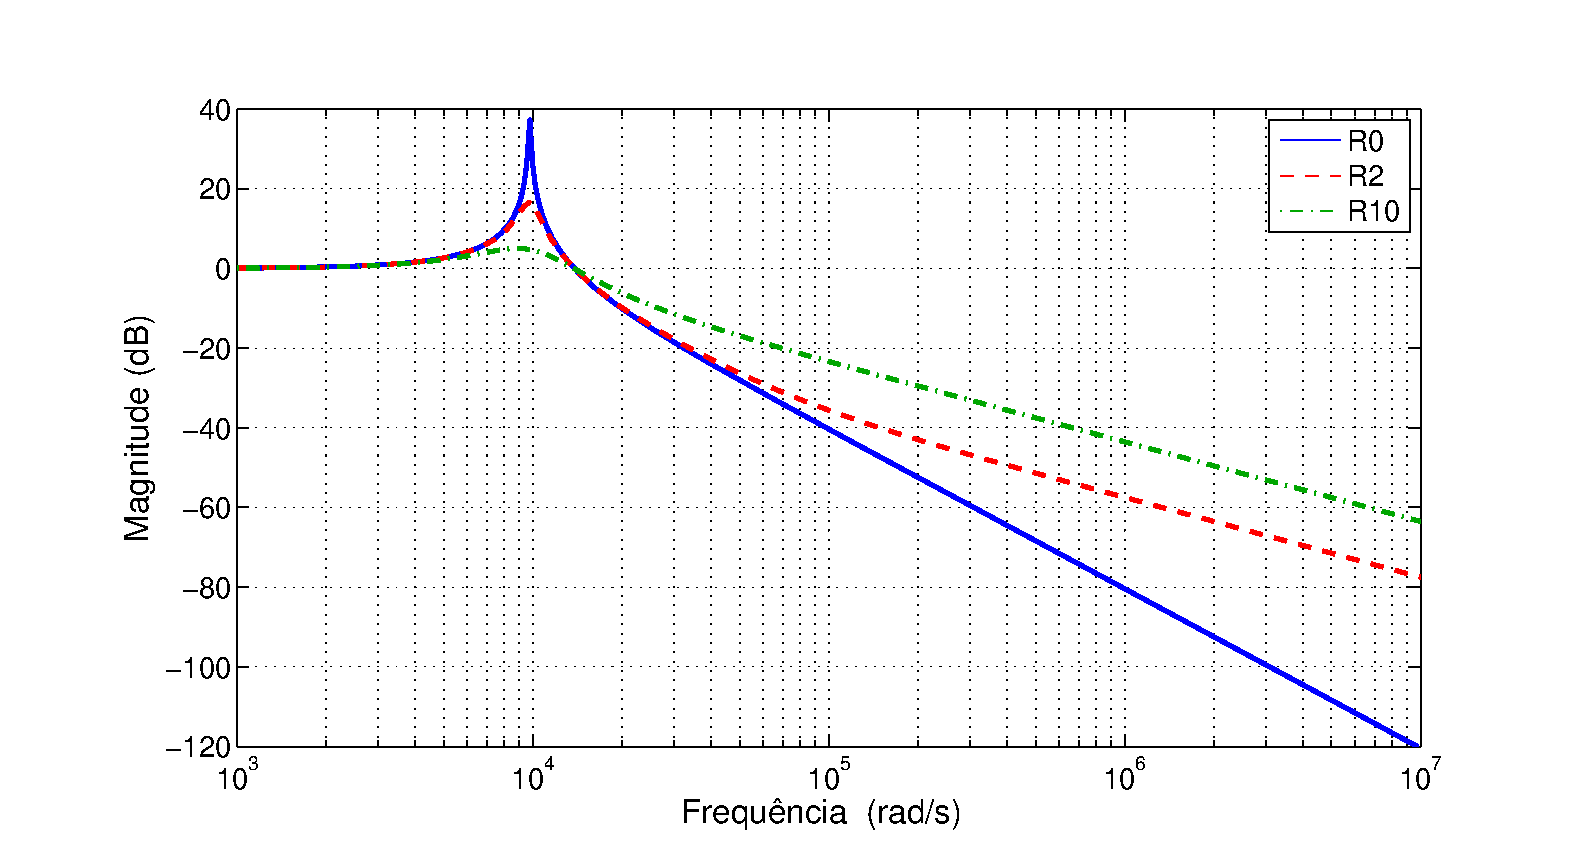
\includegraphics[width=0.9\textwidth]{img/R_in_LCL}}
            %\newlength\figureheight
		    %\newlength\figurewidth
            % This file was created by matlab2tikz v0.4.7 running on MATLAB 7.14.
% Copyright (c) 2008--2014, Nico Schlömer <nico.schloemer@gmail.com>
% All rights reserved.
% Minimal pgfplots version: 1.3
% 
% The latest updates can be retrieved from
%   http://www.mathworks.com/matlabcentral/fileexchange/22022-matlab2tikz
% where you can also make suggestions and rate matlab2tikz.
% 
%
% defining custom colors
\definecolor{mycolor1}{rgb}{0.66667,0.66667,0.66667}%
%
\begin{tikzpicture}

\begin{axis}[%
width=0.8\textwidth,
height=0.461611624834875\textwidth,
scale only axis,
xmode=log,
xmin=1000,
xmax=12589.2541179417,
xtick={1000,3162.27766016838,10000},
xticklabels={{$10^{3}$},{$10^{3.5}$},{$10^{4}$}},
xminorticks=true,
xlabel={Frequência (rad/s)},
ymin=-30,
ymax=70,
ytick={-20,   0,  20,  40,  60},
ylabel={Magnitude (dB)},
axis x line*=bottom,
axis y line*=left,
legend style={draw=black,fill=white,legend cell align=left}
]
\addplot [color=mycolor1,dash pattern=on 1pt off 3pt on 3pt off 3pt,line width=1.5pt]
  table[row sep=crcr]{1000	0.616873611257248\\
1002.30639260238	0.619383431400724\\
1004.61810465159	0.621901899176829\\
1006.93514841637	0.624429029773378\\
1009.25753619375	0.626964838250457\\
1011.58528030912	0.629509339538411\\
1013.9183931163	0.632062548435768\\
1016.2568869976	0.634624479607159\\
1018.60077436388	0.637195147581237\\
1020.95006765465	0.639774566748552\\
1023.30477933808	0.642362751359414\\
1025.66492191112	0.644959715521745\\
1028.03050789954	0.64756547319892\\
1030.40154985798	0.650180038207552\\
1032.77806037004	0.652803424215298\\
1035.16005204838	0.655435644738635\\
1037.5475375347	0.658076713140592\\
1039.94052949988	0.6607266426285\\
1042.33904064403	0.663385446251696\\
1044.74308369654	0.666053136899215\\
1047.15267141616	0.668729727297455\\
1049.56781659108	0.671415230007856\\
1051.98853203896	0.674109657424499\\
1054.41483060703	0.676813021771724\\
1056.84672517218	0.679525335101752\\
1059.28422864096	0.682246609292208\\
1061.72735394972	0.684976856043713\\
1064.17611406461	0.687716086877385\\
1066.63052198171	0.690464313132353\\
1069.09059072708	0.693221545963263\\
1071.5563333568	0.695987796337715\\
1074.02776295708	0.698763075033723\\
1076.50489264432	0.701547392637152\\
1078.98773556513	0.704340759539083\\
1081.4763048965	0.707143185933233\\
1083.97061384575	0.709954681813285\\
1086.47067565072	0.712775256970237\\
1088.97650357974	0.715604920989717\\
1091.48811093176	0.718443683249274\\
1094.00551103639	0.721291552915653\\
1096.52871725401	0.724148538942011\\
1099.05774297578	0.727014650065213\\
1101.59260162376	0.729889894802957\\
1104.13330665098	0.732774281450998\\
1106.67987154147	0.73566781808031\\
1109.2323098104	0.738570512534187\\
1111.79063500406	0.741482372425391\\
1114.35486070002	0.744403405133213\\
1116.92500050717	0.747333617800563\\
1119.50106806574	0.750273017330987\\
1122.08307704748	0.75322161038571\\
1124.67104115564	0.75617940338061\\
1127.26497412507	0.759146402483206\\
1129.86488972231	0.76212261360959\\
1132.47080174565	0.76510804242136\\
1135.0827240252	0.768102694322528\\
1137.70067042298	0.771106574456381\\
1140.32465483296	0.774119687702328\\
1142.95469118117	0.777142038672746\\
1145.59079342577	0.780173631709779\\
1148.23297555707	0.783214470882093\\
1150.8812515977	0.786264559981658\\
1153.5356356026	0.789323902520464\\
1156.19614165913	0.792392501727221\\
1158.86278388715	0.795470360544041\\
1161.53557643908	0.798557481623102\\
1164.21453349998	0.801653867323258\\
1166.89966928762	0.804759519706653\\
1169.59099805258	0.807874440535295\\
1172.28853407829	0.810998631267622\\
1174.99229168114	0.814132093054993\\
1177.70228521052	0.817274826738236\\
1180.41852904894	0.820426832844093\\
1183.14103761204	0.823588111581668\\
1185.86982534876	0.826758662838865\\
1188.60490674132	0.82993848617878\\
1191.34629630538	0.833127580836073\\
1194.09400859005	0.836325945713297\\
1196.848058178	0.839533579377246\\
1199.60845968555	0.84275048005522\\
1202.37522776272	0.845976645631315\\
1205.14837709331	0.849212073642626\\
1207.92792239501	0.85245676127551\\
1210.71387841942	0.855710705361722\\
1213.5062599522	0.8589739023746\\
1216.30508181309	0.862246348425202\\
1219.11035885602	0.865528039258384\\
1221.92210596917	0.868818970248906\\
1224.74033807505	0.87211913639746\\
1227.56507013062	0.875428532326717\\
1230.39631712731	0.878747152277296\\
1233.23409409112	0.882074990103755\\
1236.07841608273	0.885412039270514\\
1238.92929819754	0.888758292847783\\
1241.78675556577	0.892113743507443\\
1244.65080335254	0.895478383518897\\
1247.52145675793	0.898852204744914\\
1250.3987310171	0.902235198637416\\
1253.28264140034	0.905627356233271\\
1256.17320321316	0.909028668150022\\
1259.07043179635	0.912439124581617\\
1261.97434252612	0.915858715294104\\
1264.88495081411	0.919287429621277\\
1267.80227210752	0.92272525646033\\
1270.72632188919	0.92617218426745\\
1273.65711567764	0.929628201053403\\
1276.5946690272	0.933093294379093\\
1279.53899752808	0.936567451351058\\
1282.49011680643	0.940050658616987\\
1285.44804252445	0.943542902361186\\
1288.41279038047	0.947044168300005\\
1291.38437610901	0.950554441677239\\
1294.36281548089	0.95407370725954\\
1297.34812430331	0.95760194933174\\
1300.34031841991	0.961139151692182\\
1303.33941371088	0.964685297648027\\
1306.34542609305	0.96824037001051\\
1309.35837151994	0.971804351090179\\
1312.37826598188	0.975377222692105\\
1315.40512550606	0.978958966111084\\
1318.43896615665	0.982549562126752\\
1321.47980403488	0.986148990998745\\
1324.52765527909	0.989757232461779\\
1327.58253606487	0.993374265720724\\
1330.6444626051	0.997000069445648\\
1333.71345115004	1.0006346217668\\
1336.78951798747	1.00427790026965\\
1339.87267944269	1.00792988198978\\
1342.96295187868	1.01159054340787\\
1346.06035169616	1.01525986044453\\
1349.16489533366	1.01893780845527\\
1352.27659926764	1.0226243622252\\
1355.39548001256	1.02631949596401\\
1358.52155412096	1.03002318330061\\
1361.65483818355	1.03373539727799\\
1364.79534882933	1.0374561103479\\
1367.94310272563	1.04118529436555\\
1371.09811657822	1.04492292058432\\
1374.26040713143	1.04866895965039\\
1377.42999116818	1.05242338159736\\
1380.6068855101	1.05618615584082\\
1383.79110701763	1.05995725117296\\
1386.98267259009	1.06373663575708\\
1390.18159916578	1.06752427712211\\
1393.38790372205	1.07132014215709\\
1396.60160327544	1.07512419710561\\
1399.8227148817	1.0789364075603\\
1403.05125563594	1.08275673845715\\
1406.2872426727	1.08658515406997\\
1409.53069316601	1.09042161800468\\
1412.78162432955	1.09426609319365\\
1416.04005341668	1.09811854189003\\
1419.30599772055	1.10197892566198\\
1422.5794745742	1.10584720538696\\
1425.86050135065	1.1097233412459\\
1429.14909546299	1.11360729271745\\
1432.44527436445	1.11749901857213\\
1435.74905554856	1.12139847686645\\
1439.06045654914	1.12530562493709\\
1442.3794949405	1.12922041939493\\
1445.70618833745	1.13314281611919\\
1449.04055439544	1.13707277025143\\
1452.38261081064	1.1410102361896\\
1455.73237532004	1.14495516758202\\
1459.08986570152	1.14890751732139\\
1462.45509977397	1.15286723753873\\
1465.8280953974	1.1568342795973\\
1469.20887047298	1.16080859408652\\
1472.59744294318	1.16479013081588\\
1475.99383079187	1.16877883880877\\
1479.39805204436	1.17277466629635\\
1482.81012476756	1.17677756071135\\
1486.23006707006	1.18078746868191\\
1489.65789710218	1.18480433602532\\
1493.09363305612	1.1888281077418\\
1496.53729316606	1.19285872800826\\
1499.9888957082	1.19689614017198\\
1503.44845900091	1.20094028674435\\
1506.9160014048	1.20499110939453\\
1510.39154132284	1.20904854894314\\
1513.87509720044	1.21311254535589\\
1517.36668752555	1.21718303773719\\
1520.86633082875	1.2212599643238\\
1524.37404568338	1.22534326247843\\
1527.88985070559	1.22943286868326\\
1531.41376455451	1.23352871853358\\
1534.94580593225	1.23763074673128\\
1538.4859935841	1.2417388870784\\
1542.03434629857	1.24585307247067\\
1545.59088290748	1.24997323489098\\
1549.15562228612	1.25409930540291\\
1552.72858335329	1.25823121414416\\
1556.30978507143	1.26236889032007\\
1559.89924644673	1.26651226219703\\
1563.49698652918	1.27066125709594\\
1567.10302441275	1.27481580138564\\
1570.71737923542	1.27897582047634\\
1574.34007017931	1.28314123881302\\
1577.9711164708	1.28731197986886\\
1581.61053738059	1.29148796613857\\
1585.25835222385	1.29566911913187\\
1588.91458036027	1.29985535936678\\
1592.57924119422	1.30404660636307\\
1596.25235417481	1.30824277863559\\
1599.93393879601	1.3124437936876\\
1603.62401459674	1.31664956800422\\
1607.322601161	1.32086001704571\\
1611.02971811795	1.32507505524083\\
1614.74538514202	1.32929459598024\\
1618.46962195303	1.33351855160978\\
1622.20244831628	1.3377468334239\\
1625.94388404263	1.34197935165892\\
1629.69394898867	1.34621601548645\\
1633.45266305675	1.35045673300672\\
1637.22004619516	1.35470141124191\\
1640.99611839816	1.35894995612957\\
1644.78089970617	1.36320227251591\\
1648.57441020578	1.36745826414922\\
1652.37667002994	1.37171783367323\\
1656.18769935804	1.37598088262048\\
1660.00751841599	1.38024731140574\\
1663.83614747635	1.38451701931938\\
1667.67360685846	1.38878990452078\\
1671.51991692849	1.39306586403179\\
1675.37509809962	1.39734479373012\\
1679.23917083208	1.4016265883428\\
1683.11215563331	1.40591114143965\\
1686.99407305804	1.41019834542674\\
1690.88494370839	1.41448809153988\\
1694.78478823403	1.41878026983817\\
1698.69362733223	1.42307476919748\\
1702.61148174801	1.42737147730401\\
1706.53837227424	1.43167028064786\\
1710.47431975172	1.43597106451665\\
1714.41934506935	1.44027371298909\\
1718.37346916419	1.44457810892864\\
1722.33671302159	1.44888413397718\\
1726.30909767531	1.45319166854866\\
1730.2906442076	1.4575005918229\\
1734.28137374936	1.46181078173927\\
1738.28130748022	1.46612211499048\\
1742.29046662864	1.47043446701641\\
1746.30887247206	1.47474771199795\\
1750.33654633699	1.47906172285089\\
1754.37350959914	1.48337637121979\\
1758.41978368348	1.48769152747202\\
1762.47539006444	1.49200706069164\\
1766.54035026596	1.49632283867356\\
1770.61468586161	1.5006387279175\\
1774.69841847474	1.50495459362221\\
1778.79156977856	1.50927029967954\\
1782.89416149627	1.51358570866873\\
1787.00621540116	1.51790068185062\\
1791.12775331676	1.522215079162\\
1795.25879711692	1.52652875920991\\
1799.39936872594	1.53084157926614\\
1803.5494901187	1.53515339526161\\
1807.70918332073	1.53946406178096\\
1811.87847040838	1.54377343205707\\
1816.05737350894	1.54808135796579\\
1820.24591480069	1.55238769002056\\
1824.44411651309	1.55669227736721\\
1828.65200092687	1.56099496777881\\
1832.86959037413	1.56529560765054\\
1837.09690723849	1.56959404199467\\
1841.33397395519	1.57389011443559\\
1845.58081301122	1.57818366720494\\
1849.83744694544	1.58247454113677\\
1854.10389834868	1.5867625756628\\
1858.38018986386	1.5910476088078\\
1862.66634418617	1.59532947718494\\
1866.9623840631	1.59960801599137\\
1871.26833229461	1.60388305900372\\
1875.58421173328	1.60815443857383\\
1879.91004528435	1.61242198562451\\
1884.24585590593	1.61668552964534\\
1888.59166660905	1.62094489868865\\
1892.94750045783	1.62519991936554\\
1897.31338056957	1.62945041684202\\
1901.68933011491	1.63369621483524\\
1906.0753723179	1.63793713560979\\
1910.47153045619	1.64217299997419\\
1914.87782786108	1.64640362727737\\
1919.29428791772	1.65062883540535\\
1923.72093406515	1.65484844077798\\
1928.15778979652	1.65906225834582\\
1932.60487865912	1.66327010158711\\
1937.06222425457	1.66747178250486\\
1941.52985023894	1.6716671116241\\
1946.00778032282	1.67585589798915\\
1950.49603827152	1.68003794916116\\
1954.99464790516	1.68421307121564\\
1959.50363309877	1.6883810687402\\
1964.02301778248	1.69254174483237\\
1968.55282594159	1.69669490109762\\
1973.09308161673	1.70084033764743\\
1977.64380890397	1.70497785309756\\
1982.20503195496	1.70910724456643\\
1986.77677497706	1.71322830767368\\
1991.35906223344	1.71734083653884\\
1995.95191804325	1.72144462378012\\
2000.55536678172	1.72553946051346\\
2005.16943288031	1.72962513635158\\
2009.79414082682	1.73370143940334\\
2014.42951516552	1.73776815627315\\
2019.07558049731	1.74182507206056\\
2023.73236147981	1.74587197036006\\
2028.39988282751	1.74990863326101\\
2033.07816931193	1.75393484134773\\
2037.76724576168	1.7579503736998\\
2042.46713706267	1.76195500789246\\
2047.17786815819	1.7659485199973\\
2051.89946404906	1.76993068458303\\
2056.63194979376	1.77390127471648\\
2061.37535050858	1.77786006196375\\
2066.12969136771	1.78180681639158\\
2070.89499760343	1.78574130656893\\
2075.6712945062	1.78966329956868\\
2080.45860742482	1.7935725609696\\
2085.25696176653	1.79746885485845\\
2090.0663829972	1.80135194383237\\
2094.88689664142	1.80522158900137\\
2099.71852828265	1.80907754999111\\
2104.56130356336	1.81291958494584\\
2109.41524818514	1.81674745053158\\
2114.2803879089	1.82056090193949\\
2119.15674855492	1.82435969288949\\
2124.04435600306	1.82814357563407\\
2128.94323619287	1.83191230096233\\
2133.8534151237	1.83566561820423\\
2138.7749188549	1.83940327523515\\
2143.70777350589	1.84312501848055\\
2148.65200525637	1.84683059292097\\
2153.60764034637	1.8505197420972\\
2158.57470507649	1.85419220811576\\
2163.55322580795	1.85784773165453\\
2168.5432289628	1.86148605196872\\
2173.54474102401	1.86510690689698\\
2178.55778853565	1.86871003286788\\
2183.58239810298	1.87229516490655\\
2188.61859639264	1.8758620366416\\
2193.66641013278	1.87941038031231\\
2198.7258661132	1.88293992677611\\
2203.79699118545	1.8864504055162\\
2208.87981226306	1.88994154464961\\
2213.97435632161	1.89341307093539\\
2219.08065039887	1.8968647097831\\
2224.19872159503	1.90029618526166\\
2229.32859707273	1.9037072201083\\
2234.47030405729	1.90709753573801\\
2239.6238698368	1.91046685225303\\
2244.78932176229	1.91381488845285\\
2249.9666872479	1.9171413618443\\
2255.15599377096	1.92044598865206\\
2260.3572688722	1.9237284838294\\
2265.57054015585	1.92698856106921\\
2270.79583528983	1.93022593281534\\
2276.03318200585	1.93344031027423\\
2281.28260809959	1.93663140342683\\
2286.54414143084	1.93979892104082\\
2291.81780992365	1.94294257068315\\
2297.10364156645	1.94606205873284\\
2302.40166441225	1.94915709039413\\
2307.71190657875	1.95222736970991\\
2313.0343962485	1.95527259957548\\
2318.36916166905	1.95829248175258\\
2323.7162311531	1.96128671688376\\
2329.07563307865	1.96425500450707\\
2334.44739588916	1.96719704307106\\
2339.83154809368	1.97011252995007\\
2345.22811826701	1.97300116145986\\
2350.63713504986	1.97586263287355\\
2356.05862714902	1.97869663843793\\
2361.49262333744	1.98150287138997\\
2366.93915245447	1.98428102397378\\
2372.39824340596	1.98703078745783\\
2377.86992516445	1.98975185215252\\
2383.35422676926	1.99244390742802\\
2388.85117732672	1.9951066417325\\
2394.36080601029	1.99773974261068\\
2399.88314206069	2.00034289672267\\
2405.4182147861	2.00291578986316\\
2410.96605356231	2.00545810698094\\
2416.52668783283	2.00796953219874\\
2422.10014710909	2.01044974883343\\
2427.6864609706	2.01289843941648\\
2433.28565906507	2.01531528571485\\
2438.8977711086	2.01769996875209\\
2444.52282688584	2.02005216882989\\
2450.16085625011	2.02237156554987\\
2455.8118891236	2.02465783783575\\
2461.4759554975	2.02691066395581\\
2467.15308543219	2.02912972154573\\
2472.84330905736	2.03131468763168\\
2478.54665657221	2.03346523865385\\
2484.26315824557	2.03558105049019\\
2489.9928444161	2.03766179848053\\
2495.73574549243	2.03970715745105\\
2501.49189195332	2.04171680173903\\
2507.26131434783	2.04369040521793\\
2513.04404329547	2.0456276413228\\
2518.84010948637	2.04752818307604\\
2524.64954368146	2.04939170311339\\
2530.4723767126	2.05121787371035\\
2536.30863948277	2.05300636680881\\
2542.15836296621	2.05475685404408\\
2548.02157820863	2.05646900677218\\
2553.8983163273	2.05814249609743\\
2559.7886085113	2.05977699290038\\
2565.69248602162	2.06137216786605\\
2571.60998019135	2.06292769151243\\
2577.54112242586	2.0644432342193\\
2583.48594420295	2.06591846625736\\
2589.444477073	2.06735305781762\\
2595.41675265919	2.06874667904114\\
2601.4028026576	2.07009900004897\\
2607.40265883745	2.07140969097246\\
2613.41635304121	2.07267842198379\\
2619.4439171848	2.07390486332677\\
2625.48538325773	2.07508868534803\\
2631.54078332332	2.0762295585283\\
2637.61014951883	2.07732715351407\\
2643.69351405564	2.07838114114951\\
2649.7909092194	2.07939119250861\\
2655.90236737027	2.08035697892756\\
2662.02792094301	2.08127817203745\\
2668.16760244719	2.08215444379711\\
2674.32144446738	2.08298546652631\\
2680.48947966327	2.08377091293906\\
2686.67174076992	2.08451045617725\\
2692.86826059784	2.08520376984446\\
2699.07907203326	2.08585052803999\\
2705.30420803822	2.08645040539311\\
2711.54370165082	2.08700307709752\\
2717.79758598533	2.087508218946\\
2724.0658942324	2.08796550736527\\
2730.34865965925	2.08837461945102\\
2736.64591560979	2.08873523300315\\
2742.95769550488	2.08904702656115\\
2749.28403284242	2.08930967943966\\
2755.6249611976	2.08952287176424\\
2761.98051422303	2.08968628450724\\
2768.35072564895	2.08979959952384\\
2774.73562928336	2.0898624995882\\
2781.13525901229	2.08987466842984\\
2787.54964879989	2.08983579077006\\
2793.97883268864	2.08974555235847\\
2800.42284479955	2.08960364000972\\
2806.88171933232	2.0894097416403\\
2813.35549056553	2.08916354630535\\
2819.84419285683	2.08886474423571\\
2826.34786064309	2.08851302687497\\
2832.86652844062	2.08810808691656\\
2839.40023084533	2.087649618341\\
2845.94900253294	2.08713731645313\\
2852.51287825912	2.08657087791945\\
2859.09189285972	2.08595000080542\\
2865.68608125093	2.0852743846129\\
2872.29547842946	2.08454373031751\\
2878.92011947275	2.0837577404061\\
2885.56003953913	2.08291611891413\\
2892.21527386804	2.08201857146312\\
2898.88585778017	2.08106480529809\\
2905.57182667768	2.08005452932491\\
2912.27321604441	2.07898745414768\\
2918.99006144599	2.07786329210609\\
2925.72239853012	2.07668175731263\\
2932.4702630267	2.07544256568988\\
2939.23369074803	2.07414543500761\\
2946.01271758903	2.07279008491988\\
2952.80737952738	2.07137623700201\\
2959.61771262377	2.0699036147875\\
2966.44375302203	2.06837194380477\\
2973.28553694936	2.06678095161388\\
2980.14310071653	2.06513036784304\\
2987.01648071805	2.06341992422501\\
2993.90571343235	2.0616493546334\\
3000.81083542203	2.05981839511874\\
3007.73188333397	2.05792678394443\\
3014.66889389963	2.05597426162252\\
3021.62190393513	2.05396057094927\\
3028.59095034155	2.05188545704053\\
3035.57607010504	2.04974866736695\\
3042.57730029708	2.04754995178889\\
3049.59467807464	2.04528906259122\\
3056.6282406804	2.04296575451774\\
3063.67802544292	2.04057978480552\\
3070.74406977686	2.03813091321884\\
3077.82641118319	2.03561890208293\\
3084.92508724934	2.03304351631744\\
3092.04013564946	2.03040452346959\\
3099.17159414457	2.02770169374709\\
3106.3195005828	2.02493480005063\\
3113.48389289956	2.0221036180062\\
3120.66480911777	2.01920792599698\\
3127.86228734801	2.01624750519493\\
3135.0763657888	2.01322213959208\\
3142.30708272674	2.01013161603134\\
3149.55447653674	2.00697572423709\\
3156.8185856822	2.00375425684532\\
3164.09944871527	2.00046700943338\\
3171.39710427697	1.99711378054938\\
3178.71159109747	1.99369437174112\\
3186.04294799627	1.99020858758473\\
3193.39121388238	1.98665623571271\\
3200.75642775457	1.98303712684174\\
3208.13862870155	1.97935107479988\\
3215.53785590219	1.97559789655345\\
3222.9541486257	1.97177741223337\\
3230.38754623189	1.96788944516109\\
3237.83808817133	1.96393382187399\\
3245.30581398558	1.95991037215037\\
3252.79076330741	1.95581892903391\\
3260.29297586098	1.95165932885761\\
3267.81249146208	1.94743141126729\\
3275.34935001834	1.9431350192445\\
3282.90359152942	1.938769999129\\
3290.47525608724	1.9343362006406\\
3298.06438387618	1.92983347690059\\
3305.67101517332	1.92526168445253\\
3313.2951903486	1.92062068328252\\
3320.93694986511	1.91591033683895\\
3328.59633427924	1.91113051205162\\
3336.27338424092	1.90628107935036\\
3343.96814049384	1.90136191268304\\
3351.68064387566	1.89637288953299\\
3359.41093531822	1.89131389093587\\
3367.15905584778	1.88618480149588\\
3374.92504658521	1.88098550940147\\
3382.70894874623	1.87571590644037\\
3390.51080364161	1.87037588801402\\
3398.3306526774	1.86496535315143\\
3406.16853735517	1.85948420452237\\
3414.02449927217	1.85393234844999\\
3421.89858012163	1.84830969492276\\
3429.7908216929	1.84261615760583\\
3437.70126587175	1.8368516538517\\
3445.62995464054	1.83101610471034\\
3453.57693007845	1.82510943493856\\
3461.54223436172	1.81913157300882\\
3469.52590976386	1.81308245111736\\
3477.5279986559	1.80696200519167\\
3485.54854350656	1.80077017489735\\
3493.58758688252	1.7945069036443\\
3501.64517144866	1.78817213859216\\
3509.72133996824	1.78176583065531\\
3517.81613530314	1.77528793450696\\
3525.92960041413	1.76873840858277\\
3534.06177836102	1.76211721508371\\
3542.21271230298	1.75542431997829\\
3550.38244549868	1.74865969300413\\
3558.57102130658	1.74182330766885\\
3566.77848318515	1.73491514125031\\
3575.00487469309	1.72793517479621\\
3583.25023948954	1.720883393123\\
3591.51462133436	1.71375978481408\\
3599.79806408833	1.7065643422175\\
3608.10061171339	1.69929706144278\\
3616.42230827288	1.69195794235728\\
3624.76319793175	1.68454698858179\\
3633.12332495683	1.67706420748547\\
3641.50273371703	1.66950961018024\\
3649.90146868361	1.66188321151436\\
3658.31957443038	1.65418503006553\\
3666.75709563398	1.64641508813323\\
3675.21407707406	1.63857341173044\\
3683.69056363357	1.63066003057481\\
3692.18660029898	1.62267497807905\\
3700.7022321605	1.6146182913408\\
3709.23750441235	1.60649001113185\\
3717.79246235299	1.59829018188671\\
3726.36715138533	1.59001885169058\\
3734.96161701703	1.58167607226672\\
3743.57590486067	1.5732618989632\\
3752.21006063408	1.56477639073903\\
3760.86413016048	1.55621961014973\\
3769.53815936883	1.54759162333225\\
3778.23219429398	1.53889249998937\\
3786.94628107696	1.5301223133735\\
3795.68046596523	1.52128114026984\\
3804.43479531292	1.51236906097906\\
3813.20931558105	1.50338615929938\\
3822.00407333782	1.49433252250808\\
3830.81911525882	1.48520824134249\\
3839.65448812729	1.4760134099804\\
3848.51023883439	1.46674812601999\\
3857.38641437941	1.45741249045915\\
3866.28306187004	1.44800660767439\\
3875.20022852263	1.43853058539912\\
3884.13796166242	1.42898453470151\\
3893.09630872381	1.41936856996179\\
3902.07531725059	1.40968280884914\\
3911.07503489621	1.39992737229801\\
3920.09550942403	1.39010238448399\\
3929.13678870758	1.3802079727993\\
3938.19892073078	1.37024426782769\\
3947.28195358824	1.36021140331897\\
3956.38593548549	1.3501095161631\\
3965.51091473924	1.33993874636383\\
3974.65693977764	1.32969923701191\\
3983.82405914052	1.31939113425793\\
3993.0123214797	1.3090145872847\\
4002.22177555915	1.29856974827929\\
4011.45247025537	1.28805677240463\\
4020.70445455755	1.27747581777078\\
4029.97777756789	1.26682704540581\\
4039.27248850181	1.25611061922634\\
4048.58863668828	1.24532670600773\\
4057.92627157	1.23447547535389\\
4067.28544270374	1.22355709966684\\
4076.66619976054	1.21257175411587\\
4086.06859252603	1.20151961660646\\
4095.49267090063	1.19040086774886\\
4104.93848489989	1.17921569082642\\
4114.40608465467	1.16796427176357\\
4123.89552041149	1.1566467990936\\
4133.40684253274	1.14526346392617\\
4142.94010149697	1.13381445991454\\
4152.49534789915	1.12229998322257\\
4162.07263245095	1.11072023249154\\
4171.67200598098	1.09907540880669\\
4181.29351943512	1.08736571566353\\
4190.93722387671	1.07559135893407\\
4200.60317048688	1.06375254683272\\
4210.29141056481	1.05184948988211\\
4220.00199552799	1.0398824008787\\
4229.73497691249	1.02785149485819\\
4239.49040637325	1.01575698906091\\
4249.26833568435	1.0035991028969\\
4259.06881673929	0.991378057910977\\
4268.89190155123	0.97909407774768\\
4278.73764225331	0.966747388116026\\
4288.60609109892	0.954338216754218\\
4298.49730046193	0.941866793394282\\
4308.41132283705	0.929333349726571\\
4318.34821084004	0.916738119364217\\
4328.30801720801	0.904081337807536\\
4338.2907947997	0.891363242408368\\
4348.29659659578	0.878584072334332\\
4358.32547569911	0.86574406853313\\
4368.37748533501	0.852843473696752\\
4378.45267885158	0.839882532225678\\
4388.55110971994	0.826861490193095\\
4398.67283153454	0.813780595309112\\
4408.81789801347	0.800640096884929\\
4418.98636299867	0.787440245797114\\
4429.17828045629	0.774181294451814\\
4439.39370447695	0.760863496749083\\
4449.63268927599	0.747487108047186\\
4459.89528919383	0.734052385126998\\
4470.1815586962	0.720559586156416\\
4480.49155237445	0.707008970654912\\
4490.82532494586	0.693400799458072\\
4501.18293125388	0.679735334682298\\
4511.56442626847	0.666012839689538\\
4521.96986508636	0.652233579052158\\
4532.39930293136	0.638397818517874\\
4542.85279515466	0.624505824974868\\
4553.33039723509	0.610557866416928\\
4563.83216477945	0.59655421190881\\
4574.35815352278	0.582495131551669\\
4584.90841932869	0.568380896448661\\
4595.4830181896	0.55421177867066\\
4606.0820062271	0.539988051222197\\
4616.7054396922	0.525709988007461\\
4627.35337496566	0.511377863796565\\
4638.02586855826	0.496991954191918\\
4648.72297711113	0.482552535594805\\
4659.44475739604	0.468059885172125\\
4670.19126631568	0.45351428082338\\
4680.96256090399	0.438916001147763\\
4691.75869832646	0.424265325411558\\
4702.57973588042	0.40956253351566\\
4713.42573099534	0.39480790596335\\
4724.29674123316	0.380001723828261\\
4735.19282428857	0.365144268722605\\
4746.11403798933	0.350235822765588\\
4757.06044029659	0.335276668552078\\
4768.03208930514	0.320267089121511\\
4779.02904324381	0.305207367926995\\
4790.05136047569	0.290097788804741\\
4801.09909949849	0.274938635943676\\
4812.17231894485	0.259730193855307\\
4823.27107758263	0.244472747343894\\
4834.39543431522	0.229166581476844\\
4845.54544818189	0.213811981555359\\
4856.72117835806	0.198409233085406\\
4867.92268415562	0.182958621748886\\
4879.1500250233	0.167460433375129\\
4890.4032605469	0.151914953912658\\
4901.68245044966	0.136322469401221\\
4912.98765459258	0.120683265944085\\
4924.31893297469	0.10499762968069\\
4935.67634573345	0.0892658467594821\\
4947.05995314498	0.0734882033111558\\
4958.46981562442	0.0576649854220867\\
4969.90599372628	0.0417964791081302\\
4981.36854814472	0.025882970288654\\
4992.85753971387	0.00992474476095159\\
5004.37302940819	-0.00607791182513587\\
5015.91507834275	-0.022124713992214\\
5027.48374777359	-0.0382153764600792\\
5039.07909909802	-0.0543496141701343\\
5050.70119385497	-0.0705271423095186\\
5062.35009372529	-0.086747676334882\\
5074.02586053209	-0.103010931995923\\
5085.72855624109	-0.119316625358536\\
5097.45824296091	-0.135664472827711\\
5109.21498294339	-0.152054191170075\\
5120.998838584	-0.168485497536202\\
5132.80987242209	-0.184958109482465\\
5144.64814714125	-0.201471744992743\\
5156.51372556965	-0.218026122499677\\
5168.40667068035	-0.23462096090569\\
5180.32704559168	-0.251255979603658\\
5192.27491356753	-0.267930898497315\\
5204.25033801768	-0.284645438021249\\
5216.2533824982	-0.301399319160703\\
5228.28411071172	-0.318192263470945\\
5240.34258650779	-0.335023993096419\\
5252.42887388322	-0.351894230789518\\
5264.54303698246	-0.368802699929112\\
5276.68514009784	-0.38574912453865\\
5288.85524767004	-0.402733229304113\\
5301.0534242883	-0.419754739591472\\
5313.27973469088	-0.436813381463992\\
5325.53424376533	-0.45390888169913\\
5337.81701654885	-0.471040967805187\\
5350.12811822866	-0.488209368037583\\
5362.46761414231	-0.50541381141491\\
5374.83556977805	-0.522654027734596\\
5387.23205077517	-0.539929747588309\\
5399.65712292437	-0.557240702377096\\
5412.11085216805	-0.574586624326124\\
5424.59330460073	-0.59196724649918\\
5437.10454646936	-0.609382302812923\\
5449.64464417369	-0.626831528050705\\
5462.21366426659	-0.644314657876225\\
5474.81167345445	-0.661831428846835\\
5487.43873859751	-0.679381578426528\\
5500.09492671021	-0.69696484499871\\
5512.78030496154	-0.714580967878591\\
5525.49494067543	-0.73222968732536\\
5538.23890133107	-0.74991074455405\\
5551.0122545633	-0.767623881747147\\
5563.81506816292	-0.785368842065828\\
5576.64741007712	-0.803145369661067\\
5589.50934840979	-0.820953209684304\\
5602.40095142188	-0.838792108297974\\
5615.32228753178	-0.856661812685663\\
5628.2734253157	-0.874562071062098\\
5641.254433508	-0.892492632682733\\
5654.26538100157	-0.910453247853211\\
5667.30633684818	-0.928443667938442\\
5680.37737025889	-0.946463645371506\\
5693.47855060436	-0.964512933662245\\
5706.60994741527	-0.982591287405655\\
5719.77163038263	-1.00069846228991\\
5732.96366935823	-1.01883421510432\\
5746.18613435493	-1.03699830374681\\
5759.43909554709	-1.05519048723134\\
5772.72262327089	-1.07341052569501\\
5786.03678802477	-1.09165818040493\\
5799.38166046975	-1.1099332137648\\
5812.75731142982	-1.12823538932135\\
5826.16381189231	-1.14656447177045\\
5839.60123300829	-1.16492022696308\\
5853.06964609293	-1.18330242191098\\
5866.56912262587	-1.20171082479214\\
5880.09973425162	-1.22014520495603\\
5893.66155277994	-1.23860533292864\\
5907.25465018618	-1.25709098041725\\
5920.87909861173	-1.27560192031504\\
5934.53497036433	-1.29413792670545\\
5948.22233791852	-1.31269877486635\\
5961.94127391598	-1.33128424127399\\
5975.69185116595	-1.34989410360675\\
5989.47414264556	-1.36852814074865\\
6003.28822150028	-1.38718613279274\\
6017.13416104428	-1.40586786104425\\
6031.01203476082	-1.42457310802346\\
6044.92191630263	-1.44330165746857\\
6058.86387949234	-1.46205329433819\\
6072.83799832281	-1.48082780481374\\
6086.84434695757	-1.49962497630163\\
6100.88299973121	-1.51844459743536\\
6114.95403114975	-1.53728645807723\\
6129.05751589107	-1.55615034932007\\
6143.19352880526	-1.57503606348874\\
6157.36214491506	-1.59394339414139\\
6171.56343941624	-1.61287213607062\\
6185.79748767801	-1.63182208530452\\
6200.06436524339	-1.65079303910738\\
6214.36414782964	-1.66978479598043\\
6228.69691132868	-1.68879715566229\\
6243.06273180741	-1.70782991912933\\
6257.46168550822	-1.72688288859581\\
6271.89384884933	-1.74595586751402\\
6286.3592984252	-1.76504866057404\\
6300.85811100697	-1.78416107370358\\
6315.39036354283	-1.8032929140675\\
6329.95613315842	-1.82244399006734\\
6344.5554971573	-1.84161411134057\\
6359.18853302131	-1.86080308875983\\
6373.85531841099	-1.88001073443193\\
6388.55593116599	-1.89923686169681\\
6403.2904493055	-1.9184812851263\\
6418.05895102865	-1.93774382052278\\
6432.86151471491	-1.95702428491775\\
6447.69821892457	-1.97632249657023\\
6462.56914239904	-1.99563827496501\\
6477.47436406142	-2.01497144081094\\
6492.41396301678	-2.03432181603888\\
6507.38801855265	-2.05368922379973\\
6522.39661013943	-2.07307348846222\\
6537.43981743082	-2.09247443561072\\
6552.51772026422	-2.11189189204278\\
6567.63039866118	-2.13132568576671\\
6582.7779328278	-2.15077564599901\\
6597.96040315516	-2.17024160316165\\
6613.17789021976	-2.18972338887934\\
6628.43047478397	-2.20922083597667\\
6643.71823779637	-2.22873377847509\\
6659.0412603923	-2.24826205158996\\
6674.39962389419	-2.26780549172729\\
6689.79340981204	-2.2873639364806\\
6705.22269984386	-2.30693722462763\\
6720.68757587607	-2.32652519612683\\
6736.18811998395	-2.34612769211401\\
6751.7244144321	-2.36574455489873\\
6767.29654167483	-2.38537562796068\\
6782.90458435663	-2.40502075594595\\
6798.54862531262	-2.42467978466332\\
6814.22874756894	-2.44435256108034\\
6829.94503434323	-2.46403893331944\\
6845.69756904508	-2.48373875065396\\
6861.48643527643	-2.50345186350409\\
6877.31171683206	-2.52317812343273\\
6893.1734977	-2.54291738314136\\
6909.07186206198	-2.56266949646573\\
6925.00689429393	-2.58243431837168\\
6940.97867896634	-2.60221170495064\\
6956.98730084476	-2.62200151341535\\
6973.03284489025	-2.6418036020953\\
6989.11539625984	-2.66161783043231\\
7005.23504030692	-2.68144405897585\\
7021.3918625818	-2.70128214937855\\
7037.58594883204	-2.72113196439144\\
7053.81738500302	-2.74099336785928\\
7070.0862572383	-2.76086622471579\\
7086.39265188016	-2.78075040097893\\
7102.73665546999	-2.80064576374592\\
7119.11835474879	-2.82055218118852\\
7135.53783665763	-2.840469522548\\
7151.99518833808	-2.86039765813023\\
7168.49049713269	-2.88033645930069\\
7185.02385058548	-2.90028579847949\\
7201.59533644237	-2.92024554913619\\
7218.20504265165	-2.94021558578489\\
7234.85305736446	-2.96019578397894\\
7251.53946893525	-2.9801860203059\\
7268.26436592224	-3.00018617238233\\
7285.02783708792	-3.02019611884861\\
7301.82997139948	-3.04021573936366\\
7318.67085802933	-3.06024491459977\\
7335.55058635552	-3.08028352623726\\
7352.46924596225	-3.10033145695919\\
7369.42692664033	-3.12038859044607\\
7386.42371838769	-3.14045481137053\\
7403.45971140979	-3.16053000539191\\
7420.53499612018	-3.18061405915097\\
7437.64966314091	-3.20070686026442\\
7454.80380330304	-3.22080829731957\\
7471.99750764715	-3.24091825986889\\
7489.23086742376	-3.26103663842459\\
7506.50397409388	-3.28116332445316\\
7523.81691932944	-3.30129821036994\\
7541.16979501382	-3.32144118953363\\
7558.56269324229	-3.34159215624082\\
7575.99570632259	-3.36175100572055\\
7593.46892677529	-3.38191763412874\\
7610.98244733438	-3.40209193854275\\
7628.53636094773	-3.42227381695589\\
7646.13076077758	-3.44246316827186\\
7663.76574020103	-3.46265989229926\\
7681.44139281058	-3.48286388974612\\
7699.15781241454	-3.50307506221431\\
7716.91509303763	-3.52329331219407\\
7734.71332892138	-3.54351854305848\\
7752.55261452471	-3.56375065905793\\
7770.43304452438	-3.5839895653146\\
7788.35471381553	-3.60423516781698\\
7806.31771751215	-3.62448737341428\\
7824.32215094763	-3.64474608981103\\
7842.36810967519	-3.66501122556145\\
7860.45568946846	-3.68528269006402\\
7878.58498632195	-3.70556039355595\\
7896.7560964516	-3.72584424710772\\
7914.96911629522	-3.74613416261754\\
7933.22414251308	-3.76643005280595\\
7951.52127198837	-3.78673183121021\\
7969.86060182773	-3.80703941217898\\
7988.24222936175	-3.82735271086678\\
8006.66625214554	-3.84767164322858\\
8025.13276795918	-3.86799612601429\\
8043.6418748083	-3.88832607676345\\
8062.19367092452	-3.9086614137997\\
8080.78825476607	-3.92900205622544\\
8099.42572501823	-3.94934792391639\\
8118.10618059391	-3.96969893751626\\
8136.82972063413	-3.99005501843133\\
8155.5964445086	-4.01041608882512\\
8174.40645181619	-4.03078207161305\\
8193.25984238548	-4.05115289045707\\
8212.1567162753	-4.07152846976038\\
8231.09717377527	-4.09190873466217\\
8250.08131540631	-4.11229361103223\\
8269.10924192116	-4.13268302546576\\
8288.18105430498	-4.15307690527811\\
8307.29685377578	-4.17347517849952\\
8326.45674178507	-4.19387777386989\\
8345.66082001834	-4.21428462083362\\
8364.90919039556	-4.23469564953438\\
8384.20195507185	-4.25511079080999\\
8403.53921643786	-4.27552997618721\\
8422.92107712042	-4.29595313787665\\
8442.3476399831	-4.31638020876766\\
8461.81900812665	-4.33681112242322\\
8481.33528488963	-4.35724581307484\\
8500.89657384898	-4.37768421561759\\
8520.50297882047	-4.39812626560497\\
8540.15460385935	-4.41857189924394\\
8559.85155326084	-4.43902105338995\\
8579.59393156072	-4.45947366554189\\
8599.38184353586	-4.47992967383723\\
8619.21539420481	-4.50038901704703\\
8639.09468882829	-4.52085163457102\\
8659.01983290983	-4.54131746643276\\
8678.99093219629	-4.56178645327476\\
8699.00809267839	-4.58225853635357\\
8719.07142059136	-4.60273365753507\\
8739.18102241541	-4.62321175928957\\
8759.33700487634	-4.64369278468707\\
8779.5394749461	-4.66417667739251\\
8799.78853984339	-4.68466338166106\\
8820.08430703416	-4.70515284233332\\
8840.42688423224	-4.72564500483075\\
8860.81637939989	-4.74613981515092\\
8881.25290074835	-4.76663721986291\\
8901.73655673847	-4.78713716610266\\
8922.26745608124	-4.80763960156844\\
8942.84570773836	-4.82814447451621\\
8963.47142092288	-4.84865173375512\\
8984.14470509972	-4.86916132864295\\
9004.86566998624	-4.88967320908165\\
9025.63442555289	-4.91018732551284\\
9046.45108202374	-4.93070362891339\\
9067.31574987707	-4.95122207079096\\
9088.228539846	-4.97174260317962\\
9109.18956291901	-4.99226517863546\\
9130.19893034058	-5.01278975023225\\
9151.25675361173	-5.0333162715571\\
9172.36314449071	-5.0538446967062\\
9193.51821499347	-5.07437498028046\\
9214.72207739435	-5.09490707738134\\
9235.97484422661	-5.11544094360656\\
9257.27662828307	-5.13597653504595\\
9278.62754261669	-5.15651380827719\\
9300.02770054119	-5.17705272036178\\
9321.47721563161	-5.19759322884077\\
9342.97620172496	-5.21813529173078\\
9364.5247729208	-5.23867886751982\\
9386.12304358183	-5.25922391516329\\
9407.77112833455	-5.27977039407996\\
9429.46914206979	-5.30031826414792\\
9451.21719994339	-5.32086748570063\\
9473.0154173768	-5.34141801952297\\
9494.86391005764	-5.3619698268473\\
9516.76279394036	-5.38252286934951\\
9538.71218524688	-5.40307710914524\\
9560.71220046713	-5.42363250878594\\
9582.76295635973	-5.44418903125506\\
9604.86456995261	-5.46474663996427\\
9627.01715854358	-5.48530529874965\\
9649.22083970099	-5.50586497186792\\
9671.47573126437	-5.52642562399278\\
9693.78195134502	-5.54698722021111\\
9716.13961832666	-5.56754972601936\\
9738.54885086602	-5.58811310731984\\
9761.00976789355	-5.60867733041713\\
9783.52248861393	-5.62924236201444\\
9806.08713250686	-5.64980816921005\\
9828.70381932752	-5.67037471949373\\
9851.37266910737	-5.69094198074322\\
9874.09380215466	-5.7115099212207\\
9896.86733905512	-5.73207850956933\\
9919.69340067262	-5.75264771480975\\
9942.57210814977	-5.7732175063367\\
9965.5035829086	-5.79378785391553\\
9988.48794665118	-5.8143587276789\\
10011.5253213603	-5.83493009812331\\
10034.6158293	-5.85550193610584\\
10057.7595930163	-5.87607421284079\\
10080.9567353382	-5.89664689989641\\
10104.2073793774	-5.91721996919159\\
10127.5116485301	-5.9377933929927\\
10150.8696664767	-5.95836714391022\\
10174.2815571832	-5.97894119489568\\
10197.7474449012	-5.99951551923838\\
10221.267454169	-6.02009009056235\\
10244.8417098122	-6.04066488282309\\
10268.4703369442	-6.06123987030453\\
10292.1534609671	-6.08181502761595\\
10315.891207572	-6.10239032968891\\
10339.68370274	-6.12296575177418\\
10363.5310727429	-6.14354126943875\\
10387.4334441436	-6.16411685856288\\
10411.3909437969	-6.18469249533702\\
10435.4036988501	-6.20526815625896\\
10459.4718367439	-6.22584381813086\\
10483.5954852129	-6.24641945805632\\
10507.7747722864	-6.2669950534376\\
10532.0098262886	-6.28757058197262\\
10556.3007758401	-6.30814602165223\\
10580.647749858	-6.32872135075734\\
10605.0508775566	-6.34929654785612\\
10629.5102884484	-6.36987159180129\\
10654.0261123446	-6.39044646172727\\
10678.5984793556	-6.41102113704757\\
10703.2275198921	-6.43159559745195\\
10727.9133646656	-6.45216982290385\\
10752.6561446888	-6.47274379363762\\
10777.4559912768	-6.49331749015595\\
10802.3130360475	-6.51389089322724\\
10827.2274109224	-6.53446398388296\\
10852.1992481272	-6.55503674341507\\
10877.2286801926	-6.57560915337347\\
10902.315839955	-6.5961811955635\\
10927.460860557	-6.61675285204332\\
10952.6638754485	-6.63732410512147\\
10977.9250183872	-6.65789493735446\\
11003.244423439	-6.67846533154415\\
11028.6222249794	-6.69903527073542\\
11054.0585576935	-6.71960473821369\\
11079.5535565772	-6.74017371750262\\
11105.1073569377	-6.76074219236158\\
11130.7200943943	-6.7813101467834\\
11156.3919048792	-6.80187756499197\\
11182.1229246378	-6.82244443143996\\
11207.9132902301	-6.84301073080644\\
11233.7631385307	-6.8635764479947\\
11259.6726067303	-6.88414156812987\\
11285.6418323356	-6.9047060765568\\
11311.6709531708	-6.92526995883768\\
11337.7601073777	-6.94583320074995\\
11363.9094334169	-6.96639578828402\\
11390.1190700682	-6.98695770764122\\
11416.3891564316	-7.00751894523149\\
11442.7198319278	-7.02807948767135\\
11469.1112362992	-7.0486393217817\\
11495.5635096105	-7.06919843458583\\
11522.0767922492	-7.0897568133072\\
11548.6512249268	-7.11031444536748\\
11575.2869486794	-7.13087131838448\\
11601.9841048683	-7.15142742017005\\
11628.7428351806	-7.17198273872815\\
11655.5632816306	-7.19253726225281\\
11682.4455865599	-7.21309097912614\\
11709.3898926384	-7.23364387791644\\
11736.3963428651	-7.25419594737613\\
11763.4650805689	-7.27474717643994\\
11790.596249409	-7.29529755422293\\
11817.7899933763	-7.3158470700186\\
11845.0464567934	-7.33639571329704\\
11872.3657843162	-7.35694347370301\\
11899.7481209338	-7.37749034105421\\
11927.1936119701	-7.39803630533929\\
11954.7024030838	-7.41858135671614\\
11982.2746402699	-7.43912548551008\\
12009.9104698599	-7.45966868221201\\
12037.6100385228	-7.48021093747678\\
12065.3734932659	-7.50075224212127\\
12093.2009814357	-7.52129258712278\\
12121.0926507183	-7.54183196361725\\
12149.0486491407	-7.56237036289754\\
12177.069125071	-7.58290777641181\\
12205.1542272196	-7.60344419576175\\
12233.3041046402	-7.62397961270103\\
12261.5189067297	-7.64451401913354\\
12289.7987832301	-7.66504740711182\\
12318.1438842284	-7.68557976883541\\
12346.554360158	-7.70611109664934\\
12375.0303617991	-7.72664138304241\\
12403.5720402798	-7.74717062064569\\
12432.1795470765	-7.76769880223093\\
12460.8530340153	-7.78822592070908\\
12489.5926532723	-7.80875196912865\\
12518.3985573745	-7.82927694067429\\
12547.2708992008	-7.84980082866523\\
12576.2098319827	-7.87032362655382\\
12605.2155093052	-7.89084532792404\\
};
\addlegendentry{$\text{R}_\text{d}\text{ = 0}\Omega$};

\addplot [color=black!50!mycolor1,dashed,line width=1.5pt]
  table[row sep=crcr]{1000	0.719234364186966\\
1002.30639260238	0.722673811194712\\
1004.61810465159	0.726130281288975\\
1006.93514841637	0.729603864316962\\
1009.25753619375	0.73309465065479\\
1011.58528030912	0.736602731211128\\
1013.9183931163	0.740128197430885\\
1016.2568869976	0.743671141298895\\
1018.60077436388	0.747231655343675\\
1020.95006765465	0.750809832641192\\
1023.30477933808	0.754405766818641\\
1025.66492191112	0.758019552058296\\
1028.03050789954	0.761651283101382\\
1030.40154985798	0.765301055251943\\
1032.77806037004	0.768968964380784\\
1035.16005204838	0.772655106929442\\
1037.5475375347	0.776359579914163\\
1039.94052949988	0.780082480929943\\
1042.33904064403	0.783823908154593\\
1044.74308369654	0.787583960352816\\
1047.15267141616	0.791362736880347\\
1049.56781659108	0.79516033768815\\
1051.98853203896	0.798976863326568\\
1054.41483060703	0.802812414949589\\
1056.84672517218	0.806667094319123\\
1059.28422864096	0.810541003809302\\
1061.72735394972	0.814434246410825\\
1064.17611406461	0.818346925735363\\
1066.63052198171	0.822279146019931\\
1069.09059072708	0.826231012131417\\
1071.5563333568	0.830202629571017\\
1074.02776295708	0.834194104478807\\
1076.50489264432	0.838205543638323\\
1078.98773556513	0.842237054481131\\
1081.4763048965	0.846288745091541\\
1083.97061384575	0.850360724211266\\
1086.47067565072	0.854453101244156\\
1088.97650357974	0.858565986261006\\
1091.48811093176	0.862699490004346\\
1094.00551103639	0.866853723893311\\
1096.52871725401	0.871028800028535\\
1099.05774297578	0.87522483119713\\
1101.59260162376	0.879441930877627\\
1104.13330665098	0.883680213245051\\
1106.67987154147	0.887939793175982\\
1109.2323098104	0.892220786253666\\
1111.79063500406	0.896523308773206\\
1114.35486070002	0.900847477746758\\
1116.92500050717	0.905193410908795\\
1119.50106806574	0.909561226721414\\
1122.08307704748	0.913951044379687\\
1124.67104115564	0.918362983817067\\
1127.26497412507	0.922797165710824\\
1129.86488972231	0.927253711487559\\
1132.47080174565	0.931732743328732\\
1135.0827240252	0.936234384176269\\
1137.70067042298	0.940758757738211\\
1140.32465483296	0.945305988494401\\
1142.95469118117	0.949876201702231\\
1145.59079342577	0.95446952340245\\
1148.23297555707	0.959086080425019\\
1150.8812515977	0.963726000394996\\
1153.5356356026	0.968389411738512\\
1156.19614165913	0.973076443688776\\
1158.86278388715	0.977787226292138\\
1161.53557643908	0.982521890414227\\
1164.21453349998	0.9872805677461\\
1166.89966928762	0.992063390810499\\
1169.59099805258	0.996870492968137\\
1172.28853407829	1.00170200842403\\
1174.99229168114	1.00655807223394\\
1177.70228521052	1.01143882031078\\
1180.41852904894	1.01634438943121\\
1183.14103761204	1.02127491724215\\
1185.86982534876	1.0262305422675\\
1188.60490674132	1.03121140391477\\
1191.34629630538	1.03621764248189\\
1194.09400859005	1.04124939916406\\
1196.848058178	1.04630681606059\\
1199.60845968555	1.05139003618189\\
1202.37522776272	1.05649920345653\\
1205.14837709331	1.06163446273823\\
1207.92792239501	1.06679595981311\\
1210.71387841942	1.07198384140688\\
1213.5062599522	1.0771982551921\\
1216.30508181309	1.08243934979558\\
1219.11035885602	1.08770727480578\\
1221.92210596917	1.09300218078033\\
1224.74033807505	1.09832421925356\\
1227.56507013062	1.10367354274417\\
1230.39631712731	1.10905030476294\\
1233.23409409112	1.11445465982051\\
1236.07841608273	1.11988676343521\\
1238.92929819754	1.12534677214103\\
1241.78675556577	1.1308348434956\\
1244.65080335254	1.13635113608832\\
1247.52145675793	1.14189580954846\\
1250.3987310171	1.14746902455343\\
1253.28264140034	1.15307094283709\\
1256.17320321316	1.15870172719818\\
1259.07043179635	1.16436154150874\\
1261.97434252612	1.17005055072273\\
1264.88495081411	1.1757689208846\\
1267.80227210752	1.18151681913812\\
1270.72632188919	1.18729441373508\\
1273.65711567764	1.19310187404425\\
1276.5946690272	1.19893937056036\\
1279.53899752808	1.20480707491313\\
1282.49011680643	1.21070515987647\\
1285.44804252445	1.21663379937772\\
1288.41279038047	1.22259316850693\\
1291.38437610901	1.22858344352638\\
1294.36281548089	1.23460480188003\\
1297.34812430331	1.24065742220314\\
1300.34031841991	1.24674148433203\\
1303.33941371088	1.25285716931381\\
1306.34542609305	1.25900465941633\\
1309.35837151994	1.26518413813816\\
1312.37826598188	1.27139579021868\\
1315.40512550606	1.2776398016483\\
1318.43896615665	1.28391635967869\\
1321.47980403488	1.2902256528333\\
1324.52765527909	1.29656787091772\\
1327.58253606487	1.30294320503041\\
1330.6444626051	1.3093518475733\\
1333.71345115004	1.31579399226272\\
1336.78951798747	1.32226983414024\\
1339.87267944269	1.32877956958375\\
1342.96295187868	1.33532339631858\\
1346.06035169616	1.34190151342882\\
1349.16489533366	1.34851412136858\\
1352.27659926764	1.3551614219736\\
1355.39548001256	1.36184361847277\\
1358.52155412096	1.36856091549988\\
1361.65483818355	1.37531351910546\\
1364.79534882933	1.38210163676872\\
1367.94310272563	1.38892547740967\\
1371.09811657822	1.39578525140124\\
1374.26040713143	1.40268117058172\\
1377.42999116818	1.40961344826711\\
1380.6068855101	1.41658229926376\\
1383.79110701763	1.42358793988106\\
1386.98267259009	1.43063058794426\\
1390.18159916578	1.43771046280746\\
1393.38790372205	1.44482778536672\\
1396.60160327544	1.45198277807327\\
1399.8227148817	1.45917566494689\\
1403.05125563594	1.46640667158945\\
1406.2872426727	1.47367602519852\\
1409.53069316601	1.48098395458117\\
1412.78162432955	1.48833069016794\\
1416.04005341668	1.49571646402686\\
1419.30599772055	1.50314150987772\\
1422.5794745742	1.51060606310644\\
1425.86050135065	1.51811036077954\\
1429.14909546299	1.52565464165889\\
1432.44527436445	1.53323914621648\\
1435.74905554856	1.54086411664943\\
1439.06045654914	1.54852979689509\\
1442.3794949405	1.55623643264639\\
1445.70618833745	1.56398427136727\\
1449.04055439544	1.57177356230827\\
1452.38261081064	1.57960455652237\\
1455.73237532004	1.58747750688089\\
1459.08986570152	1.59539266808966\\
1462.45509977397	1.60335029670524\\
1465.8280953974	1.61135065115142\\
1469.20887047298	1.61939399173588\\
1472.59744294318	1.62748058066695\\
1475.99383079187	1.63561068207061\\
1479.39805204436	1.64378456200768\\
1482.81012476756	1.65200248849116\\
1486.23006707006	1.66026473150376\\
1489.65789710218	1.66857156301562\\
1493.09363305612	1.67692325700226\\
1496.53729316606	1.68532008946262\\
1499.9888957082	1.69376233843742\\
1503.44845900091	1.70225028402761\\
1506.9160014048	1.71078420841307\\
1510.39154132284	1.71936439587154\\
1513.87509720044	1.72799113279764\\
1517.36668752555	1.73666470772224\\
1520.86633082875	1.74538541133196\\
1524.37404568338	1.75415353648882\\
1527.88985070559	1.76296937825026\\
1531.41376455451	1.77183323388925\\
1534.94580593225	1.78074540291463\\
1538.4859935841	1.78970618709173\\
1542.03434629857	1.79871589046317\\
1545.59088290748	1.80777481936987\\
1549.15562228612	1.81688328247233\\
1552.72858335329	1.82604159077214\\
1556.30978507143	1.83525005763368\\
1559.89924644673	1.84450899880607\\
1563.49698652918	1.85381873244541\\
1567.10302441275	1.86317957913719\\
1570.71737923542	1.872591861919\\
1574.34007017931	1.88205590630346\\
1577.9711164708	1.89157204030139\\
1581.61053738059	1.90114059444527\\
1585.25835222385	1.91076190181293\\
1588.91458036027	1.92043629805152\\
1592.57924119422	1.93016412140167\\
1596.25235417481	1.93994571272207\\
1599.93393879601	1.94978141551413\\
1603.62401459674	1.95967157594706\\
1607.322601161	1.96961654288314\\
1611.02971811795	1.97961666790332\\
1614.74538514202	1.98967230533305\\
1618.46962195303	1.99978381226846\\
1622.20244831628	2.00995154860274\\
1625.94388404263	2.0201758770529\\
1629.69394898867	2.03045716318678\\
1633.45266305675	2.04079577545036\\
1637.22004619516	2.05119208519533\\
1640.99611839816	2.06164646670709\\
1644.78089970617	2.07215929723291\\
1648.57441020578	2.08273095701051\\
1652.37667002994	2.09336182929686\\
1656.18769935804	2.1040523003974\\
1660.00751841599	2.11480275969551\\
1663.83614747635	2.12561359968234\\
1667.67360685846	2.13648521598691\\
1671.51991692849	2.14741800740669\\
1675.37509809962	2.15841237593827\\
1679.23917083208	2.16946872680866\\
1683.11215563331	2.18058746850668\\
1686.99407305804	2.19176901281489\\
1690.88494370839	2.2030137748417\\
1694.78478823403	2.21432217305401\\
1698.69362733223	2.22569462931003\\
1702.61148174801	2.23713156889265\\
1706.53837227424	2.24863342054299\\
1710.47431975172	2.26020061649447\\
1714.41934506935	2.27183359250716\\
1718.37346916419	2.28353278790255\\
1722.33671302159	2.2952986455987\\
1726.30909767531	2.30713161214572\\
1730.2906442076	2.3190321377618\\
1734.28137374936	2.33100067636936\\
1738.28130748022	2.3430376856319\\
1742.29046662864	2.35514362699103\\
1746.30887247206	2.36731896570399\\
1750.33654633699	2.37956417088159\\
1754.37350959914	2.39187971552655\\
1758.41978368348	2.40426607657221\\
1762.47539006444	2.41672373492175\\
1766.54035026596	2.42925317548777\\
1770.61468586161	2.44185488723226\\
1774.69841847474	2.45452936320716\\
1778.79156977856	2.46727710059515\\
1782.89416149627	2.48009860075106\\
1787.00621540116	2.49299436924357\\
1791.12775331676	2.5059649158975\\
1795.25879711692	2.51901075483644\\
1799.39936872594	2.53213240452589\\
1803.5494901187	2.54533038781685\\
1807.70918332073	2.55860523198984\\
1811.87847040838	2.57195746879946\\
1816.05737350894	2.58538763451933\\
1820.24591480069	2.59889626998755\\
1824.44411651309	2.61248392065262\\
1828.65200092687	2.62615113661991\\
1832.86959037413	2.63989847269844\\
1837.09690723849	2.65372648844836\\
1841.33397395519	2.6676357482287\\
1845.58081301122	2.68162682124585\\
1849.83744694544	2.69570028160229\\
1854.10389834868	2.70985670834602\\
1858.38018986386	2.72409668552032\\
1862.66634418617	2.73842080221417\\
1866.9623840631	2.75282965261304\\
1871.26833229461	2.76732383605025\\
1875.58421173328	2.78190395705884\\
1879.91004528435	2.79657062542396\\
1884.24585590593	2.81132445623568\\
1888.59166660905	2.82616606994245\\
1892.94750045783	2.84109609240497\\
1897.31338056957	2.85611515495059\\
1901.68933011491	2.8712238944283\\
1906.0753723179	2.88642295326413\\
1910.47153045619	2.90171297951712\\
1914.87782786108	2.91709462693583\\
1919.29428791772	2.93256855501529\\
1923.72093406515	2.94813542905455\\
1928.15778979652	2.9637959202147\\
1932.60487865912	2.97955070557738\\
1937.06222425457	2.99540046820384\\
1941.52985023894	3.01134589719453\\
1946.00778032282	3.02738768774909\\
1950.49603827152	3.04352654122697\\
1954.99464790516	3.05976316520851\\
1959.50363309877	3.07609827355645\\
1964.02301778248	3.09253258647798\\
1968.55282594159	3.10906683058734\\
1973.09308161673	3.1257017389688\\
1977.64380890397	3.14243805124014\\
1982.20503195496	3.15927651361666\\
1986.77677497706	3.17621787897556\\
1991.35906223344	3.19326290692083\\
1995.95191804325	3.21041236384861\\
2000.55536678172	3.22766702301289\\
2005.16943288031	3.24502766459173\\
2009.79414082682	3.26249507575387\\
2014.42951516552	3.28007005072567\\
2019.07558049731	3.29775339085855\\
2023.73236147981	3.31554590469674\\
2028.39988282751	3.33344840804539\\
2033.07816931193	3.35146172403904\\
2037.76724576168	3.36958668321042\\
2042.46713706267	3.38782412355955\\
2047.17786815819	3.40617489062313\\
2051.89946404906	3.42463983754419\\
2056.63194979376	3.44321982514199\\
2061.37535050858	3.46191572198219\\
2066.12969136771	3.48072840444713\\
2070.89499760343	3.49965875680635\\
2075.6712945062	3.51870767128721\\
2080.45860742482	3.53787604814568\\
2085.25696176653	3.55716479573711\\
2090.0663829972	3.57657483058716\\
2094.88689664142	3.5961070774627\\
2099.71852828265	3.61576246944262\\
2104.56130356336	3.63554194798866\\
2109.41524818514	3.65544646301611\\
2114.2803879089	3.6754769729643\\
2119.15674855492	3.69563444486696\\
2124.04435600306	3.71591985442233\\
2128.94323619287	3.73633418606286\\
2133.8534151237	3.7568784330247\\
2138.7749188549	3.77755359741665\\
2143.70777350589	3.79836069028868\\
2148.65200525637	3.81930073169995\\
2153.60764034637	3.84037475078609\\
2158.57470507649	3.86158378582592\\
2163.55322580795	3.88292888430734\\
2168.5432289628	3.90441110299239\\
2173.54474102401	3.92603150798135\\
2178.55778853565	3.94779117477592\\
2183.58239810298	3.96969118834114\\
2188.61859639264	3.99173264316623\\
2193.66641013278	4.01391664332404\\
2198.7258661132	4.03624430252909\\
2203.79699118545	4.05871674419409\\
2208.87981226306	4.08133510148479\\
2213.97435632161	4.10410051737302\\
2219.08065039887	4.12701414468782\\
2224.19872159503	4.15007714616456\\
2229.32859707273	4.17329069449174\\
2234.47030405729	4.19665597235551\\
2239.6238698368	4.2201741724817\\
2244.78932176229	4.24384649767498\\
2249.9666872479	4.26767416085534\\
2255.15599377096	4.29165838509139\\
2260.3572688722	4.31580040363039\\
2265.57054015585	4.34010145992485\\
2270.79583528983	4.36456280765547\\
2276.03318200585	4.38918571074999\\
2281.28260809959	4.41397144339812\\
2286.54414143084	4.43892129006183\\
2291.81780992365	4.4640365454811\\
2297.10364156645	4.48931851467461\\
2302.40166441225	4.51476851293533\\
2307.71190657875	4.5403878658203\\
2313.0343962485	4.56617790913479\\
2318.36916166905	4.59213998891005\\
2323.7162311531	4.61827546137456\\
2329.07563307865	4.64458569291832\\
2334.44739588916	4.67107206004986\\
2339.83154809368	4.69773594934532\\
2345.22811826701	4.72457875738958\\
2350.63713504986	4.75160189070858\\
2356.05862714902	4.77880676569262\\
2361.49262333744	4.80619480851003\\
2366.93915245447	4.83376745501076\\
2372.39824340596	4.8615261506192\\
2377.86992516445	4.88947235021591\\
2383.35422676926	4.91760751800729\\
2388.85117732672	4.94593312738303\\
2394.36080601029	4.97445066076022\\
2399.88314206069	5.00316160941371\\
2405.4182147861	5.03206747329189\\
2410.96605356231	5.06116976081721\\
2416.52668783283	5.09046998867043\\
2422.10014710909	5.11996968155808\\
2427.6864609706	5.14967037196195\\
2433.28565906507	5.17957359986987\\
2438.8977711086	5.20968091248667\\
2444.52282688584	5.23999386392457\\
2450.16085625011	5.2705140148715\\
2455.8118891236	5.30124293223664\\
2461.4759554975	5.33218218877191\\
2467.15308543219	5.36333336266786\\
2472.84330905736	5.39469803712323\\
2478.54665657221	5.42627779988634\\
2484.26315824557	5.45807424276714\\
2489.9928444161	5.49008896111839\\
2495.73574549243	5.5223235532844\\
2501.49189195332	5.55477962001561\\
2507.26131434783	5.58745876384752\\
2513.04404329547	5.62036258844199\\
2518.84010948637	5.65349269788895\\
2524.64954368146	5.68685069596687\\
2530.4723767126	5.72043818535964\\
2536.30863948277	5.75425676682772\\
2542.15836296621	5.78830803833137\\
2548.02157820863	5.82259359410372\\
2553.8983163273	5.85711502367071\\
2559.7886085113	5.89187391081582\\
2565.69248602162	5.92687183248668\\
2571.60998019135	5.96211035764032\\
2577.54112242586	5.99759104602474\\
2583.48594420295	6.03331544689301\\
2589.444477073	6.06928509764699\\
2595.41675265919	6.10550152240702\\
2601.4028026576	6.14196623050418\\
2607.40265883745	6.17868071489096\\
2613.41635304121	6.21564645046681\\
2619.4439171848	6.25286489231406\\
2625.48538325773	6.29033747384007\\
2631.54078332332	6.32806560482105\\
2637.61014951883	6.36605066934269\\
2643.69351405564	6.40429402363268\\
2649.7909092194	6.44279699377999\\
2655.90236737027	6.48156087333534\\
2662.02792094301	6.52058692078725\\
2668.16760244719	6.55987635690786\\
2674.32144446738	6.59943036196191\\
2680.48947966327	6.6392500727729\\
2686.67174076992	6.6793365796394\\
2692.86826059784	6.71969092309433\\
2699.07907203326	6.76031409050018\\
2705.30420803822	6.80120701247224\\
2711.54370165082	6.84237055912182\\
2717.79758598533	6.88380553611127\\
2724.0658942324	6.92551268051211\\
2730.34865965925	6.96749265645692\\
2736.64591560979	7.00974605057604\\
2742.95769550488	7.05227336720901\\
2749.28403284242	7.09507502338047\\
2755.6249611976	7.13815134353039\\
2761.98051422303	7.18150255398733\\
2768.35072564895	7.22512877717335\\
2774.73562928336	7.2690300255291\\
2781.13525901229	7.31320619514674\\
2787.54964879989	7.35765705909801\\
2793.97883268864	7.40238226044463\\
2800.42284479955	7.44738130491768\\
2806.88171933232	7.49265355325181\\
2813.35549056553	7.53819821316049\\
2819.84419285683	7.58401433093752\\
2826.34786064309	7.63010078266962\\
2832.86652844062	7.6764562650453\\
2839.40023084533	7.72307928574387\\
2845.94900253294	7.76996815338881\\
2852.51287825912	7.81712096704934\\
2859.09189285972	7.86453560527375\\
2865.68608125093	7.91220971463748\\
2872.29547842946	7.96014069778985\\
2878.92011947275	8.00832570098182\\
2885.56003953913	8.05676160105857\\
2892.21527386804	8.10544499189978\\
2898.88585778017	8.15437217029124\\
2905.57182667768	8.20353912121125\\
2912.27321604441	8.25294150251623\\
2918.99006144599	8.30257462900998\\
2925.72239853012	8.35243345588203\\
2932.4702630267	8.40251256150129\\
2939.23369074803	8.45280612955236\\
2946.01271758903	8.50330793050271\\
2952.80737952738	8.55401130239124\\
2959.61771262377	8.60490913092955\\
2966.44375302203	8.65599382890994\\
2973.28553694936	8.7072573149163\\
2980.14310071653	8.75869099133663\\
2987.01648071805	8.81028572167882\\
2993.90571343235	8.86203180719563\\
3000.81083542203	8.91391896282711\\
3007.73188333397	8.96593629247485\\
3014.66889389963	9.01807226362586\\
3021.62190393513	9.07031468134993\\
3028.59095034155	9.12265066170033\\
3035.57607010504	9.17506660455403\\
3042.57730029708	9.22754816593486\\
3049.59467807464	9.28008022987132\\
3056.6282406804	9.33264687984895\\
3063.67802544292	9.38523136992683\\
3070.74406977686	9.43781609559798\\
3077.82641118319	9.49038256448453\\
3084.92508724934	9.54291136696993\\
3092.04013564946	9.59538214688389\\
3099.17159414457	9.64777357236883\\
3106.3195005828	9.70006330707093\\
3113.48389289956	9.7522279818145\\
3120.66480911777	9.80424316693444\\
3127.86228734801	9.85608334545748\\
3135.0763657888	9.90772188734184\\
3142.30708272674	9.9591310250018\\
3149.55447653674	10.0102818303626\\
3156.8185856822	10.0611441937103\\
3164.09944871527	10.1116868046203\\
3171.39710427697	10.1618771352663\\
3178.71159109747	10.2116814264322\\
3186.04294799627	10.2610646765665\\
3193.39121388238	10.3099906342349\\
3200.75642775457	10.3584217943481\\
3208.13862870155	10.4063193985494\\
3215.53785590219	10.4536434401662\\
3222.9541486257	10.5003526741354\\
3230.38754623189	10.5464046323229\\
3237.83808817133	10.5917556446588\\
3245.30581398558	10.636360866513\\
3252.79076330741	10.6801743127271\\
3260.29297586098	10.7231488987138\\
3267.81249146208	10.7652364890131\\
3275.34935001834	10.8063879536787\\
3282.90359152942	10.8465532328339\\
3290.47525608724	10.8856814097032\\
3298.06438387618	10.9237207923798\\
3305.67101517332	10.9606190045363\\
3313.2951903486	10.9963230852276\\
3320.93694986511	11.0307795978602\\
3328.59633427924	11.0639347483301\\
3336.27338424092	11.0957345122395\\
3343.96814049384	11.1261247710123\\
3351.68064387566	11.1550514566228\\
3359.41093531822	11.1824607045484\\
3367.15905584778	11.208299014439\\
3374.92504658521	11.2325134178823\\
3382.70894874623	11.255051652523\\
3390.51080364161	11.2758623416739\\
3398.3306526774	11.2948951784385\\
3406.16853735517	11.3121011132523\\
3414.02449927217	11.3274325436364\\
3421.89858012163	11.3408435048658\\
3429.7908216929	11.3522898601567\\
3437.70126587175	11.3617294889122\\
3445.62995464054	11.3691224714996\\
3453.57693007845	11.3744312689969\\
3461.54223436172	11.3776208963248\\
3469.52590976386	11.3786590871826\\
3477.5279986559	11.3775164492315\\
3485.54854350656	11.3741666080177\\
3493.58758688252	11.3685863382007\\
3501.64517144866	11.3607556807494\\
3509.72133996824	11.3506580448859\\
3517.81613530314	11.3382802937017\\
3525.92960041413	11.3236128125258\\
3534.06177836102	11.3066495593059\\
3542.21271230298	11.2873880964504\\
3550.38244549868	11.2658296037825\\
3558.57102130658	11.2419788724614\\
3566.77848318515	11.2158442799408\\
3575.00487469309	11.1874377462373\\
3583.25023948954	11.1567746719898\\
3591.51462133436	11.123873858983\\
3599.79806408833	11.0887574139907\\
3608.10061171339	11.0514506369605\\
3616.42230827288	11.0119818947107\\
3624.76319793175	10.9703824814363\\
3633.12332495683	10.9266864674264\\
3641.50273371703	10.8809305374769\\
3649.90146868361	10.8331538205406\\
3658.31957443038	10.7833977121888\\
3666.75709563398	10.7317056914716\\
3675.21407707406	10.6781231337477\\
3683.69056363357	10.622697121027\\
3692.18660029898	10.5654762513116\\
3700.7022321605	10.5065104483563\\
3709.23750441235	10.4458507731836\\
3717.79246235299	10.3835492385927\\
3726.36715138533	10.3196586277988\\
3734.96161701703	10.254232318222\\
3743.57590486067	10.1873241113336\\
3752.21006063408	10.1189880693427\\
3760.86413016048	10.0492783593897\\
3769.53815936883	9.97824910579303\\
3778.23219429398	9.90595425078164\\
3786.94628107696	9.83244742403461\\
3795.68046596523	9.75778182124638\\
3804.43479531292	9.68201009183766\\
3813.20931558105	9.60518423584405\\
3822.00407333782	9.52735550993129\\
3830.81911525882	9.44857434241562\\
3839.65448812729	9.36889025710135\\
3848.51023883439	9.2883518056934\\
3857.38641437941	9.20700650849552\\
3866.28306187004	9.12490080306405\\
3875.20022852263	9.04208000045714\\
3884.13796166242	8.9585882486942\\
3893.09630872381	8.87446850302162\\
3902.07531725059	8.78976250256996\\
3911.07503489621	8.70451075298118\\
3920.09550942403	8.61875251458134\\
3929.13678870758	8.53252579567934\\
3938.19892073078	8.44586735057575\\
3947.28195358824	8.35881268187719\\
3956.38593548549	8.27139604672249\\
3965.51091473924	8.18365046654214\\
3974.65693977764	8.09560773998654\\
3983.82405914052	8.0072984586781\\
3993.0123214797	7.91875202545801\\
4002.22177555915	7.82999667481883\\
4011.45247025537	7.74105949523202\\
4020.70445455755	7.65196645309986\\
4029.97777756789	7.5627424180782\\
4039.27248850181	7.47341118953795\\
4048.58863668828	7.38399552394874\\
4057.92627157	7.29451716298783\\
4067.28544270374	7.20499686219341\\
4076.66619976054	7.1154544199985\\
4086.06859252603	7.02590870699584\\
4095.49267090063	6.93637769530097\\
4104.93848489989	6.84687848789234\\
4114.40608465467	6.75742734782185\\
4123.89552041149	6.66803972720079\\
4133.40684253274	6.57873029587772\\
4142.94010149697	6.48951296973454\\
4152.49534789915	6.40040093853833\\
4162.07263245095	6.31140669329346\\
4171.67200598098	6.22254205304826\\
4181.29351943512	6.13381819111715\\
4190.93722387671	6.04524566068658\\
4200.60317048688	5.9568344197783\\
4210.29141056481	5.8685938555505\\
4220.00199552799	5.78053280792099\\
4229.73497691249	5.69265959250205\\
4239.49040637325	5.60498202284021\\
4249.26833568435	5.51750743195821\\
4259.06881673929	5.43024269319852\\
4268.89190155123	5.34319424037252\\
4278.73764225331	5.25636808721948\\
4288.60609109892	5.16976984618371\\
4298.49730046193	5.08340474651918\\
4308.41132283705	4.99727765173214\\
4318.34821084004	4.91139307637428\\
4328.30801720801	4.82575520220019\\
4338.2907947997	4.7403678937029\\
4348.29659659578	4.65523471304274\\
4358.32547569911	4.57035893438578\\
4368.37748533501	4.48574355766726\\
4378.45267885158	4.40139132179668\\
4388.55110971994	4.31730471732184\\
4398.67283153454	4.23348599856781\\
4408.81789801347	4.14993719526808\\
4418.98636299867	4.06666012370502\\
4429.17828045629	3.98365639737551\\
4439.39370447695	3.90092743719932\\
4449.63268927599	3.81847448128555\\
4459.89528919383	3.736298594274\\
4470.1815586962	3.65440067626655\\
4480.49155237445	3.5727814713648\\
4490.82532494586	3.49144157582804\\
4501.18293125388	3.41038144586739\\
4511.56442626847	3.32960140508948\\
4521.96986508636	3.24910165160431\\
4532.39930293136	3.1688822648103\\
4542.85279515466	3.08894321187044\\
4553.33039723509	3.0092843538911\\
4563.83216477945	2.92990545181722\\
4574.35815352278	2.85080617205446\\
4584.90841932869	2.77198609183085\\
4595.4830181896	2.69344470430819\\
4606.0820062271	2.61518142345487\\
4616.7054396922	2.53719558868914\\
4627.35337496566	2.4594864693042\\
4638.02586855826	2.38205326868332\\
4648.72297711113	2.30489512831516\\
4659.44475739604	2.22801113161734\\
4670.19126631568	2.15140030757759\\
4680.96256090399	2.07506163421953\\
4691.75869832646	1.99899404190202\\
4702.57973588042	1.92319641645859\\
4713.42573099534	1.84766760218475\\
4724.29674123316	1.77240640467966\\
4735.19282428857	1.69741159354919\\
4746.11403798933	1.62268190497604\\
4757.06044029659	1.54821604416368\\
4768.03208930514	1.47401268765922\\
4779.02904324381	1.4000704855611\\
4790.05136047569	1.32638806361703\\
4801.09909949849	1.2529640252168\\
4812.17231894485	1.17979695328493\\
4823.27107758263	1.10688541207826\\
4834.39543431522	1.03422794889214\\
4845.54544818189	0.961823095679875\\
4856.72117835806	0.889669370589608\\
4867.92268415562	0.817765279421997\\
4879.1500250233	0.746109317012704\\
4890.4032605469	0.674699968543339\\
4901.68245044966	0.603535710783824\\
4912.98765459258	0.532615013269495\\
4924.31893297469	0.461936339416479\\
4935.67634573345	0.391498147577298\\
4947.05995314498	0.321298892040658\\
4958.46981562442	0.251337023977006\\
4969.90599372628	0.181610992333143\\
4981.36854814472	0.112119244677807\\
4992.85753971387	0.0428602280011453\\
5004.37302940819	-0.0261676105305985\\
5015.91507834275	-0.0949658228620583\\
5027.48374777359	-0.163535959376305\\
5039.07909909802	-0.231879568260403\\
5050.70119385497	-0.299998194907618\\
5062.35009372529	-0.367893381353991\\
5074.02586053209	-0.43556666574835\\
5085.72855624109	-0.503019581853373\\
5097.45824296091	-0.570253658576847\\
5109.21498294339	-0.63727041953128\\
5120.998838584	-0.704071382620808\\
5132.80987242209	-0.770658059653543\\
5144.64814714125	-0.837031955978963\\
5156.51372556965	-0.903194570148176\\
5168.40667068035	-0.969147393596767\\
5180.32704559168	-1.0348919103486\\
5192.27491356753	-1.10042959673987\\
5204.25033801768	-1.16576192116202\\
5216.2533824982	-1.2308903438232\\
5228.28411071172	-1.29581631652662\\
5240.34258650779	-1.36054128246564\\
5252.42887388322	-1.42506667603429\\
5264.54303698246	-1.48939392265282\\
5276.68514009784	-1.55352443860699\\
5288.85524767004	-1.61745963090128\\
5301.0534242883	-1.6812008971242\\
5313.27973469088	-1.74474962532622\\
5325.53424376533	-1.8081071939088\\
5337.81701654885	-1.87127497152456\\
5350.12811822866	-1.93425431698748\\
5362.46761414231	-1.99704657919323\\
5374.83556977805	-2.05965309704847\\
5387.23205077517	-2.12207519940914\\
5399.65712292437	-2.18431420502718\\
5412.11085216805	-2.24637142250483\\
5424.59330460073	-2.30824815025675\\
5437.10454646936	-2.36994567647915\\
5449.64464417369	-2.43146527912546\\
5462.21366426659	-2.49280822588858\\
5474.81167345445	-2.55397577418909\\
5487.43873859751	-2.61496917116897\\
5500.09492671021	-2.67578965369097\\
5512.78030496154	-2.73643844834275\\
5525.49494067543	-2.79691677144607\\
5538.23890133107	-2.85722582907031\\
5551.0122545633	-2.91736681705043\\
5563.81506816292	-2.97734092100869\\
5576.64741007712	-3.03714931638046\\
5589.50934840979	-3.09679316844328\\
5602.40095142188	-3.15627363234948\\
5615.32228753178	-3.21559185316186\\
5628.2734253157	-3.27474896589244\\
5641.254433508	-3.33374609554365\\
5654.26538100157	-3.39258435715261\\
5667.30633684818	-3.45126485583735\\
5680.37737025889	-3.50978868684559\\
5693.47855060436	-3.56815693560562\\
5706.60994741527	-3.62637067777909\\
5719.77163038263	-3.68443097931557\\
5732.96366935823	-3.74233889650904\\
5746.18613435493	-3.80009547605573\\
5759.43909554709	-3.85770175511356\\
5772.72262327089	-3.91515876136295\\
5786.03678802477	-3.97246751306888\\
5799.38166046975	-4.02962901914394\\
5812.75731142982	-4.08664427921276\\
5826.16381189231	-4.14351428367703\\
5839.60123300829	-4.20024001378172\\
5853.06964609293	-4.25682244168188\\
5866.56912262587	-4.31326253051037\\
5880.09973425162	-4.36956123444592\\
5893.66155277994	-4.42571949878219\\
5907.25465018618	-4.48173825999688\\
5920.87909861173	-4.53761844582166\\
5934.53497036433	-4.59336097531228\\
5948.22233791852	-4.64896675891913\\
5961.94127391598	-4.70443669855791\\
5975.69185116595	-4.75977168768075\\
5989.47414264556	-4.81497261134728\\
6003.28822150028	-4.87004034629598\\
6017.13416104428	-4.92497576101562\\
6031.01203476082	-4.9797797158166\\
6044.92191630263	-5.03445306290246\\
6058.86387949234	-5.08899664644134\\
6072.83799832281	-5.14341130263721\\
6086.84434695757	-5.19769785980122\\
6100.88299973121	-5.25185713842287\\
6114.95403114975	-5.30588995124087\\
6129.05751589107	-5.35979710331398\\
6143.19352880526	-5.41357939209171\\
6157.36214491506	-5.46723760748446\\
6171.56343941624	-5.52077253193377\\
6185.79748767801	-5.57418494048214\\
6200.06436524339	-5.62747560084246\\
6214.36414782964	-5.68064527346733\\
6228.69691132868	-5.73369471161783\\
6243.06273180741	-5.78662466143212\\
6257.46168550822	-5.83943586199355\\
6271.89384884933	-5.89212904539857\\
6286.3592984252	-5.9447049368239\\
6300.85811100697	-5.99716425459376\\
6315.39036354283	-6.04950771024625\\
6329.95613315842	-6.10173600859959\\
6344.5554971573	-6.15384984781782\\
6359.18853302131	-6.20584991947608\\
6373.85531841099	-6.25773690862534\\
6388.55593116599	-6.30951149385689\\
6403.2904493055	-6.36117434736608\\
6418.05895102865	-6.41272613501581\\
6432.86151471491	-6.46416751639942\\
6447.69821892457	-6.51549914490322\\
6462.56914239904	-6.56672166776829\\
6477.47436406142	-6.61783572615213\\
6492.41396301678	-6.66884195518943\\
6507.38801855265	-6.7197409840527\\
6522.39661013943	-6.7705334360121\\
6537.43981743082	-6.82121992849504\\
6552.51772026422	-6.87180107314497\\
6567.63039866118	-6.92227747587997\\
6582.7779328278	-6.97264973695054\\
6597.96040315516	-7.02291845099714\\
6613.17789021976	-7.07308420710702\\
6628.43047478397	-7.12314758887072\\
6643.71823779637	-7.17310917443778\\
6659.0412603923	-7.22296953657236\\
6674.39962389419	-7.27272924270789\\
6689.79340981204	-7.32238885500151\\
6705.22269984386	-7.371948930388\\
6720.68757587607	-7.42141002063301\\
6736.18811998395	-7.47077267238591\\
6751.7244144321	-7.52003742723225\\
6767.29654167483	-7.56920482174542\\
6782.90458435663	-7.61827538753807\\
6798.54862531262	-7.66724965131303\\
6814.22874756894	-7.71612813491348\\
6829.94503434323	-7.76491135537291\\
6845.69756904508	-7.81359982496448\\
6861.48643527643	-7.86219405124985\\
6877.31171683206	-7.91069453712757\\
6893.1734977	-7.95910178088106\\
6909.07186206198	-8.0074162762259\\
6925.00689429393	-8.05563851235695\\
6940.97867896634	-8.10376897399467\\
6956.98730084476	-8.15180814143122\\
6973.03284489025	-8.19975649057598\\
6989.11539625984	-8.24761449300071\\
7005.23504030692	-8.295382615984\\
7021.3918625818	-8.34306132255562\\
7037.58594883204	-8.39065107154013\\
7053.81738500302	-8.43815231760016\\
7070.0862572383	-8.48556551127927\\
7086.39265188016	-8.53289109904435\\
7102.73665546999	-8.58012952332747\\
7119.11835474879	-8.62728122256752\\
7135.53783665763	-8.67434663125118\\
7151.99518833808	-8.72132617995366\\
7168.49049713269	-8.76822029537885\\
7185.02385058548	-8.81502940039929\\
7201.59533644237	-8.86175391409537\\
7218.20504265165	-8.90839425179452\\
7234.85305736446	-8.95495082510964\\
7251.53946893525	-9.00142404197739\\
7268.26436592224	-9.04781430669588\\
7285.02783708792	-9.09412201996221\\
7301.82997139948	-9.14034757890926\\
7318.67085802933	-9.18649137714253\\
7335.55058635552	-9.23255380477618\\
7352.46924596225	-9.27853524846896\\
7369.42692664033	-9.32443609145966\\
7386.42371838769	-9.37025671360231\\
7403.45971140979	-9.41599749140073\\
7420.53499612018	-9.46165879804306\\
7437.64966314091	-9.50724100343569\\
7454.80380330304	-9.55274447423689\\
7471.99750764715	-9.5981695738902\\
7489.23086742376	-9.64351666265728\\
7506.50397409388	-9.68878609765055\\
7523.81691932944	-9.7339782328655\\
7541.16979501382	-9.77909341921253\\
7558.56269324229	-9.82413200454853\\
7575.99570632259	-9.86909433370829\\
7593.46892677529	-9.9139807485352\\
7610.98244733438	-9.95879158791202\\
7628.53636094773	-10.0035271877911\\
7646.13076077758	-10.0481878812245\\
7663.76574020103	-10.0927739983931\\
7681.44139281058	-10.1372858666369\\
7699.15781241454	-10.181723810483\\
7716.91509303763	-10.2260881516752\\
7734.71332892138	-10.2703792092018\\
7752.55261452471	-10.3145972993242\\
7770.43304452438	-10.3587427356043\\
7788.35471381553	-10.4028158289325\\
7806.31771751215	-10.4468168875548\\
7824.32215094763	-10.4907462170995\\
7842.36810967519	-10.5346041206043\\
7860.45568946846	-10.5783908985427\\
7878.58498632195	-10.6221068488496\\
7896.7560964516	-10.665752266948\\
7914.96911629522	-10.7093274457741\\
7933.22414251308	-10.7528326758025\\
7951.52127198837	-10.7962682450719\\
7969.86060182773	-10.8396344392093\\
7988.24222936175	-10.8829315414548\\
8006.66625214554	-10.9261598326862\\
8025.13276795918	-10.9693195914425\\
8043.6418748083	-11.0124110939482\\
8062.19367092452	-11.0554346141366\\
8080.78825476607	-11.0983904236733\\
8099.42572501823	-11.141278791979\\
8118.10618059391	-11.1840999862528\\
8136.82972063413	-11.2268542714944\\
8155.5964445086	-11.2695419105269\\
8174.40645181619	-11.3121631640185\\
8193.25984238548	-11.3547182905047\\
8212.1567162753	-11.3972075464101\\
8231.09717377527	-11.4396311860696\\
8250.08131540631	-11.4819894617499\\
8269.10924192116	-11.5242826236705\\
8288.18105430498	-11.5665109200247\\
8307.29685377578	-11.6086745969997\\
8326.45674178507	-11.6507738987976\\
8345.66082001834	-11.6928090676556\\
8364.90919039556	-11.7347803438654\\
8384.20195507185	-11.7766879657937\\
8403.53921643786	-11.8185321699015\\
8422.92107712042	-11.8603131907636\\
8442.3476399831	-11.9020312610876\\
8461.81900812665	-11.9436866117333\\
8481.33528488963	-11.9852794717312\\
8500.89657384898	-12.0268100683014\\
8520.50297882047	-12.068278626872\\
8540.15460385935	-12.109685371097\\
8559.85155326084	-12.1510305228752\\
8579.59393156072	-12.1923143023674\\
8599.38184353586	-12.2335369280143\\
8619.21539420481	-12.2746986165543\\
8639.09468882829	-12.3157995830408\\
8659.01983290983	-12.3568400408591\\
8678.99093219629	-12.3978202017439\\
8699.00809267839	-12.438740275796\\
8719.07142059136	-12.4796004714989\\
8739.18102241541	-12.5204009957355\\
8759.33700487634	-12.5611420538044\\
8779.5394749461	-12.6018238494361\\
8799.78853984339	-12.6424465848093\\
8820.08430703416	-12.6830104605665\\
8840.42688423224	-12.7235156758298\\
8860.81637939989	-12.7639624282167\\
8881.25290074835	-12.8043509138555\\
8901.73655673847	-12.8446813274004\\
8922.26745608124	-12.8849538620467\\
8942.84570773836	-12.9251687095461\\
8963.47142092288	-12.9653260602211\\
8984.14470509972	-13.0054261029801\\
9004.86566998624	-13.0454690253317\\
9025.63442555289	-13.0854550133994\\
9046.45108202374	-13.1253842519354\\
9067.31574987707	-13.1652569243354\\
9088.228539846	-13.2050732126522\\
9109.18956291901	-13.2448332976095\\
9130.19893034058	-13.284537358616\\
9151.25675361173	-13.3241855737787\\
9172.36314449071	-13.3637781199166\\
9193.51821499347	-13.4033151725739\\
9214.72207739435	-13.4427969060333\\
9235.97484422661	-13.482223493329\\
9257.27662828307	-13.52159510626\\
9278.62754261669	-13.5609119154023\\
9300.02770054119	-13.6001740901225\\
9321.47721563161	-13.6393817985895\\
9342.97620172496	-13.6785352077878\\
9364.5247729208	-13.7176344835292\\
9386.12304358183	-13.7566797904655\\
9407.77112833455	-13.7956712921004\\
9429.46914206979	-13.8346091508017\\
9451.21719994339	-13.8734935278129\\
9473.0154173768	-13.9123245832653\\
9494.86391005764	-13.9511024761897\\
9516.76279394036	-13.9898273645275\\
9538.71218524688	-14.0284994051429\\
9560.71220046713	-14.0671187538334\\
9582.76295635973	-14.105685565342\\
9604.86456995261	-14.1441999933673\\
9627.01715854358	-14.1826621905754\\
9649.22083970099	-14.2210723086104\\
9671.47573126437	-14.2594304981054\\
9693.78195134502	-14.297736908693\\
9716.13961832666	-14.3359916890161\\
9738.54885086602	-14.3741949867384\\
9761.00976789355	-14.4123469485549\\
9783.52248861393	-14.450447720202\\
9806.08713250686	-14.488497446468\\
9828.70381932752	-14.5264962712031\\
9851.37266910737	-14.5644443373293\\
9874.09380215466	-14.6023417868506\\
9896.86733905512	-14.6401887608628\\
9919.69340067262	-14.6779853995631\\
9942.57210814977	-14.71573184226\\
9965.5035829086	-14.7534282273824\\
9988.48794665118	-14.79107469249\\
10011.5253213603	-14.8286713742816\\
10034.6158293	-14.8662184086053\\
10057.7595930163	-14.9037159304673\\
10080.9567353382	-14.9411640740409\\
10104.2073793774	-14.978562972676\\
10127.5116485301	-15.0159127589079\\
10150.8696664767	-15.0532135644657\\
10174.2815571832	-15.090465520282\\
10197.7474449012	-15.1276687565009\\
10221.267454169	-15.1648234024868\\
10244.8417098122	-15.2019295868331\\
10268.4703369442	-15.2389874373708\\
10292.1534609671	-15.2759970811764\\
10315.891207572	-15.3129586445806\\
10339.68370274	-15.3498722531766\\
10363.5310727429	-15.3867380318279\\
10387.4334441436	-15.4235561046768\\
10411.3909437969	-15.4603265951522\\
10435.4036988501	-15.4970496259773\\
10459.4718367439	-15.5337253191782\\
10483.5954852129	-15.5703537960906\\
10507.7747722864	-15.6069351773686\\
10532.0098262886	-15.6434695829917\\
10556.3007758401	-15.6799571322725\\
10580.647749858	-15.7163979438641\\
10605.0508775566	-15.7527921357679\\
10629.5102884484	-15.7891398253406\\
10654.0261123446	-15.8254411293015\\
10678.5984793556	-15.86169616374\\
10703.2275198921	-15.8979050441224\\
10727.9133646656	-15.9340678852993\\
10752.6561446888	-15.9701848015124\\
10777.4559912768	-16.0062559064014\\
10802.3130360475	-16.0422813130113\\
10827.2274109224	-16.0782611337986\\
10852.1992481272	-16.1141954806386\\
10877.2286801926	-16.1500844648317\\
10902.315839955	-16.1859281971104\\
10927.460860557	-16.2217267876454\\
10952.6638754485	-16.2574803460526\\
10977.9250183872	-16.2931889813991\\
11003.244423439	-16.3288528022099\\
11028.6222249794	-16.3644719164741\\
11054.0585576935	-16.4000464316509\\
11079.5535565772	-16.4355764546765\\
11105.1073569377	-16.4710620919692\\
11130.7200943943	-16.5065034494365\\
11156.3919048792	-16.5419006324804\\
11182.1229246378	-16.5772537460039\\
11207.9132902301	-16.6125628944162\\
11233.7631385307	-16.6478281816393\\
11259.6726067303	-16.6830497111134\\
11285.6418323356	-16.7182275858027\\
11311.6709531708	-16.7533619082009\\
11337.7601073777	-16.7884527803371\\
11363.9094334169	-16.8235003037813\\
11390.1190700682	-16.8585045796497\\
11416.3891564316	-16.8934657086105\\
11442.7198319278	-16.928383790889\\
11469.1112362992	-16.963258926273\\
11495.5635096105	-16.9980912141182\\
11522.0767922492	-17.0328807533535\\
11548.6512249268	-17.067627642486\\
11575.2869486794	-17.1023319796063\\
11601.9841048683	-17.1369938623933\\
11628.7428351806	-17.1716133881197\\
11655.5632816306	-17.2061906536567\\
11682.4455865599	-17.2407257554788\\
11709.3898926384	-17.2752187896691\\
11736.3963428651	-17.3096698519238\\
11763.4650805689	-17.344079037557\\
11790.596249409	-17.3784464415056\\
11817.7899933763	-17.412772158334\\
11845.0464567934	-17.4470562822386\\
11872.3657843162	-17.4812989070523\\
11899.7481209338	-17.5155001262496\\
11927.1936119701	-17.5496600329502\\
11954.7024030838	-17.5837787199244\\
11982.2746402699	-17.6178562795969\\
12009.9104698599	-17.6518928040512\\
12037.6100385228	-17.6858883850342\\
12065.3734932659	-17.7198431139605\\
12093.2009814357	-17.7537570819161\\
12121.0926507183	-17.7876303796632\\
12149.0486491407	-17.8214630976439\\
12177.069125071	-17.8552553259847\\
12205.1542272196	-17.8890071544999\\
12233.3041046402	-17.9227186726966\\
12261.5189067297	-17.9563899697777\\
12289.7987832301	-17.9900211346463\\
12318.1438842284	-18.0236122559095\\
12346.554360158	-18.0571634218824\\
12375.0303617991	-18.0906747205915\\
12403.5720402798	-18.1241462397789\\
12432.1795470765	-18.1575780669056\\
12460.8530340153	-18.1909702891556\\
12489.5926532723	-18.2243229934391\\
12518.3985573745	-18.2576362663965\\
12547.2708992008	-18.2909101944017\\
12576.2098319827	-18.3241448635657\\
12605.2155093052	-18.3573403597399\\
};
\addlegendentry{$\text{R}_\text{d}\text{ = 2}\Omega$};

\addplot [color=black,solid,line width=1.5pt]
  table[row sep=crcr]{1000	0.724243453088894\\
1002.30639260238	0.727732183831662\\
1004.61810465159	0.7312384374546\\
1006.93514841637	0.734762309098373\\
1009.25753619375	0.738303894492078\\
1011.58528030912	0.741863289957599\\
1013.9183931163	0.745440592414038\\
1016.2568869976	0.749035899382135\\
1018.60077436388	0.752649308988783\\
1020.95006765465	0.756280919971544\\
1023.30477933808	0.759930831683227\\
1025.66492191112	0.763599144096495\\
1028.03050789954	0.767285957808538\\
1030.40154985798	0.770991374045754\\
1032.77806037004	0.774715494668505\\
1035.16005204838	0.778458422175899\\
1037.5475375347	0.782220259710626\\
1039.94052949988	0.786001111063826\\
1042.33904064403	0.789801080680026\\
1044.74308369654	0.793620273662096\\
1047.15267141616	0.797458795776262\\
1049.56781659108	0.801316753457189\\
1051.98853203896	0.805194253813066\\
1054.41483060703	0.809091404630767\\
1056.84672517218	0.813008314381083\\
1059.28422864096	0.816945092223939\\
1061.72735394972	0.82090184801373\\
1064.17611406461	0.824878692304667\\
1066.63052198171	0.828875736356175\\
1069.09059072708	0.832893092138366\\
1071.5563333568	0.836930872337542\\
1074.02776295708	0.840989190361753\\
1076.50489264432	0.845068160346426\\
1078.98773556513	0.849167897160028\\
1081.4763048965	0.853288516409786\\
1083.97061384575	0.857430134447481\\
1086.47067565072	0.861592868375271\\
1088.97650357974	0.865776836051593\\
1091.48811093176	0.869982156097107\\
1094.00551103639	0.87420894790071\\
1096.52871725401	0.878457331625588\\
1099.05774297578	0.882727428215364\\
1101.59260162376	0.887019359400266\\
1104.13330665098	0.891333247703369\\
1106.67987154147	0.895669216446934\\
1109.2323098104	0.900027389758734\\
1111.79063500406	0.904407892578522\\
1114.35486070002	0.908810850664499\\
1116.92500050717	0.913236390599905\\
1119.50106806574	0.91768463979961\\
1122.08307704748	0.922155726516832\\
1124.67104115564	0.926649779849888\\
1127.26497412507	0.931166929749007\\
1129.86488972231	0.935707307023245\\
1132.47080174565	0.94027104334743\\
1135.0827240252	0.944858271269195\\
1137.70067042298	0.949469124216107\\
1140.32465483296	0.954103736502803\\
1142.95469118117	0.958762243338265\\
1145.59079342577	0.96344478083314\\
1148.23297555707	0.968151486007123\\
1150.8812515977	0.972882496796437\\
1153.5356356026	0.977637952061378\\
1156.19614165913	0.982417991593939\\
1158.86278388715	0.987222756125504\\
1161.53557643908	0.992052387334654\\
1164.21453349998	0.996907027854998\\
1166.89966928762	1.00178682128313\\
1169.59099805258	1.00669191218666\\
1172.28853407829	1.0116224461123\\
1174.99229168114	1.01657856959407\\
1177.70228521052	1.0215604301616\\
1180.41852904894	1.02656817634843\\
1183.14103761204	1.0316019577005\\
1185.86982534876	1.03666192478472\\
1188.60490674132	1.04174822919752\\
1191.34629630538	1.04686102357362\\
1194.09400859005	1.05200046159486\\
1196.848058178	1.05716669799903\\
1199.60845968555	1.06235988858894\\
1202.37522776272	1.06758019024148\\
1205.14837709331	1.0728277609168\\
1207.92792239501	1.07810275966764\\
1210.71387841942	1.08340534664864\\
1213.5062599522	1.08873568312593\\
1216.30508181309	1.09409393148661\\
1219.11035885602	1.09948025524853\\
1221.92210596917	1.10489481907003\\
1224.74033807505	1.11033778875986\\
1227.56507013062	1.11580933128719\\
1230.39631712731	1.12130961479173\\
1233.23409409112	1.12683880859394\\
1236.07841608273	1.13239708320538\\
1238.92929819754	1.13798461033915\\
1241.78675556577	1.1436015629205\\
1244.65080335254	1.14924811509744\\
1247.52145675793	1.15492444225156\\
1250.3987310171	1.16063072100899\\
1253.28264140034	1.16636712925139\\
1256.17320321316	1.17213384612712\\
1259.07043179635	1.17793105206254\\
1261.97434252612	1.18375892877338\\
1264.88495081411	1.18961765927632\\
1267.80227210752	1.19550742790063\\
1270.72632188919	1.20142842029995\\
1273.65711567764	1.20738082346426\\
1276.5946690272	1.21336482573188\\
1279.53899752808	1.21938061680174\\
1282.49011680643	1.22542838774562\\
1285.44804252445	1.23150833102073\\
1288.41279038047	1.23762064048223\\
1291.38437610901	1.24376551139605\\
1294.36281548089	1.24994314045175\\
1297.34812430331	1.25615372577562\\
1300.34031841991	1.26239746694383\\
1303.33941371088	1.26867456499582\\
1306.34542609305	1.27498522244776\\
1309.35837151994	1.28132964330628\\
1312.37826598188	1.2877080330822\\
1315.40512550606	1.29412059880461\\
1318.43896615665	1.30056754903489\\
1321.47980403488	1.30704909388115\\
1324.52765527909	1.31356544501258\\
1327.58253606487	1.32011681567417\\
1330.6444626051	1.3267034207015\\
1333.71345115004	1.33332547653571\\
1336.78951798747	1.33998320123868\\
1339.87267944269	1.34667681450839\\
1342.96295187868	1.35340653769441\\
1346.06035169616	1.36017259381361\\
1349.16489533366	1.36697520756608\\
1352.27659926764	1.3738146053512\\
1355.39548001256	1.38069101528393\\
1358.52155412096	1.38760466721125\\
1361.65483818355	1.39455579272886\\
1364.79534882933	1.40154462519802\\
1367.94310272563	1.40857139976268\\
1371.09811657822	1.41563635336667\\
1374.26040713143	1.4227397247713\\
1377.42999116818	1.42988175457296\\
1380.6068855101	1.43706268522108\\
1383.79110701763	1.44428276103631\\
1386.98267259009	1.45154222822879\\
1390.18159916578	1.45884133491681\\
1393.38790372205	1.46618033114559\\
1396.60160327544	1.47355946890632\\
1399.8227148817	1.48097900215545\\
1403.05125563594	1.48843918683423\\
1406.2872426727	1.49594028088843\\
1409.53069316601	1.50348254428838\\
1412.78162432955	1.51106623904923\\
1416.04005341668	1.51869162925144\\
1419.30599772055	1.52635898106159\\
1422.5794745742	1.53406856275335\\
1425.86050135065	1.54182064472883\\
1429.14909546299	1.54961549954016\\
1432.44527436445	1.55745340191126\\
1435.74905554856	1.56533462876002\\
1439.06045654914	1.57325945922069\\
1442.3794949405	1.58122817466656\\
1445.70618833745	1.58924105873292\\
1449.04055439544	1.59729839734037\\
1452.38261081064	1.60540047871838\\
1455.73237532004	1.61354759342916\\
1459.08986570152	1.62174003439184\\
1462.45509977397	1.62997809690701\\
1465.8280953974	1.6382620786815\\
1469.20887047298	1.64659227985355\\
1472.59744294318	1.65496900301829\\
1475.99383079187	1.66339255325351\\
1479.39805204436	1.67186323814588\\
1482.81012476756	1.68038136781735\\
1486.23006707006	1.6889472549521\\
1489.65789710218	1.69756121482364\\
1493.09363305612	1.70622356532248\\
1496.53729316606	1.71493462698394\\
1499.9888957082	1.72369472301658\\
1503.44845900091	1.73250417933079\\
1506.9160014048	1.74136332456791\\
1510.39154132284	1.75027249012967\\
1513.87509720044	1.75923201020808\\
1517.36668752555	1.76824222181565\\
1520.86633082875	1.77730346481613\\
1524.37404568338	1.78641608195555\\
1527.88985070559	1.79558041889378\\
1531.41376455451	1.80479682423647\\
1534.94580593225	1.81406564956745\\
1538.4859935841	1.82338724948155\\
1542.03434629857	1.83276198161793\\
1545.59088290748	1.84219020669382\\
1549.15562228612	1.85167228853874\\
1552.72858335329	1.86120859412921\\
1556.30978507143	1.87079949362395\\
1559.89924644673	1.88044536039955\\
1563.49698652918	1.89014657108667\\
1567.10302441275	1.89990350560669\\
1570.71737923542	1.909716547209\\
1574.34007017931	1.91958608250868\\
1577.9711164708	1.92951250152482\\
1581.61053738059	1.93949619771932\\
1585.25835222385	1.94953756803628\\
1588.91458036027	1.95963701294195\\
1592.57924119422	1.96979493646526\\
1596.25235417481	1.98001174623891\\
1599.93393879601	1.99028785354108\\
1603.62401459674	2.00062367333776\\
1607.322601161	2.01101962432562\\
1611.02971811795	2.02147612897563\\
1614.74538514202	2.03199361357719\\
1618.46962195303	2.04257250828302\\
1622.20244831628	2.05321324715461\\
1625.94388404263	2.06391626820843\\
1629.69394898867	2.07468201346278\\
1633.45266305675	2.08551092898532\\
1637.22004619516	2.09640346494136\\
1640.99611839816	2.10736007564285\\
1644.78089970617	2.11838121959806\\
1648.57441020578	2.12946735956211\\
1652.37667002994	2.14061896258812\\
1656.18769935804	2.15183650007931\\
1660.00751841599	2.16312044784171\\
1663.83614747635	2.17447128613783\\
1667.67360685846	2.18588949974102\\
1671.51991692849	2.1973755779908\\
1675.37509809962	2.20893001484887\\
1679.23917083208	2.22055330895615\\
1683.11215563331	2.23224596369062\\
1686.99407305804	2.24400848722605\\
1690.88494370839	2.25584139259165\\
1694.78478823403	2.26774519773274\\
1698.69362733223	2.2797204255722\\
1702.61148174801	2.29176760407305\\
1706.53837227424	2.30388726630193\\
1710.47431975172	2.31607995049359\\
1714.41934506935	2.32834620011643\\
1718.37346916419	2.34068656393908\\
1722.33671302159	2.35310159609801\\
1726.30909767531	2.36559185616626\\
1730.2906442076	2.37815790922329\\
1734.28137374936	2.39080032592587\\
1738.28130748022	2.40351968258021\\
1742.29046662864	2.41631656121525\\
1746.30887247206	2.42919154965707\\
1750.33654633699	2.44214524160459\\
1754.37350959914	2.45517823670652\\
1758.41978368348	2.46829114063948\\
1762.47539006444	2.48148456518752\\
1766.54035026596	2.49475912832289\\
1770.61468586161	2.50811545428818\\
1774.69841847474	2.5215541736798\\
1778.79156977856	2.53507592353291\\
1782.89416149627	2.54868134740771\\
1787.00621540116	2.56237109547723\\
1791.12775331676	2.57614582461661\\
1795.25879711692	2.5900061984938\\
1799.39936872594	2.60395288766195\\
1803.5494901187	2.61798656965328\\
1807.70918332073	2.63210792907456\\
1811.87847040838	2.64631765770426\\
1816.05737350894	2.66061645459138\\
1820.24591480069	2.67500502615596\\
1824.44411651309	2.68948408629134\\
1828.65200092687	2.70405435646827\\
1832.86959037413	2.71871656584071\\
1837.09690723849	2.73347145135362\\
1841.33397395519	2.74831975785254\\
1845.58081301122	2.76326223819523\\
1849.83744694544	2.77829965336514\\
1854.10389834868	2.79343277258703\\
1858.38018986386	2.80866237344455\\
1862.66634418617	2.82398924200008\\
1866.9623840631	2.83941417291651\\
1871.26833229461	2.85493796958141\\
1875.58421173328	2.87056144423335\\
1879.91004528435	2.8862854180906\\
1884.24585590593	2.90211072148202\\
1888.59166660905	2.91803819398057\\
1892.94750045783	2.93406868453909\\
1897.31338056957	2.95020305162866\\
1901.68933011491	2.96644216337957\\
1906.0753723179	2.98278689772481\\
1910.47153045619	2.99923814254632\\
1914.87782786108	3.01579679582395\\
1919.29428791772	3.03246376578721\\
1923.72093406515	3.04923997106993\\
1928.15778979652	3.06612634086779\\
1932.60487865912	3.0831238150989\\
1937.06222425457	3.1002333445674\\
1941.52985023894	3.11745589113027\\
1946.00778032282	3.13479242786725\\
1950.49603827152	3.15224393925412\\
1954.99464790516	3.16981142133933\\
1959.50363309877	3.18749588192402\\
1964.02301778248	3.20529834074562\\
1968.55282594159	3.22321982966504\\
1973.09308161673	3.24126139285749\\
1977.64380890397	3.25942408700715\\
1982.20503195496	3.27770898150572\\
1986.77677497706	3.29611715865478\\
1991.35906223344	3.31464971387239\\
1995.95191804325	3.33330775590376\\
2000.55536678172	3.3520924070361\\
2005.16943288031	3.37100480331795\\
2009.79414082682	3.39004609478294\\
2014.42951516552	3.409217445678\\
2019.07558049731	3.42852003469645\\
2023.73236147981	3.44795505521574\\
2028.39988282751	3.46752371554015\\
2033.07816931193	3.48722723914855\\
2037.76724576168	3.50706686494733\\
2042.46713706267	3.52704384752856\\
2047.17786815819	3.5471594574337\\
2051.89946404906	3.56741498142274\\
2056.63194979376	3.58781172274916\\
2061.37535050858	3.60835100144069\\
2066.12969136771	3.62903415458611\\
2070.89499760343	3.64986253662815\\
2075.6712945062	3.6708375196628\\
2080.45860742482	3.69196049374502\\
2085.25696176653	3.71323286720116\\
2090.0663829972	3.73465606694818\\
2094.88689664142	3.75623153881991\\
2099.71852828265	3.77796074790045\\
2104.56130356336	3.79984517886504\\
2109.41524818514	3.82188633632841\\
2114.2803879089	3.844085745201\\
2119.15674855492	3.86644495105312\\
2124.04435600306	3.8889655204874\\
2128.94323619287	3.91164904151958\\
2133.8534151237	3.93449712396801\\
2138.7749188549	3.95751139985207\\
2143.70777350589	3.98069352379974\\
2148.65200525637	4.00404517346452\\
2153.60764034637	4.0275680499521\\
2158.57470507649	4.05126387825683\\
2163.55322580795	4.07513440770865\\
2168.5432289628	4.09918141243017\\
2173.54474102401	4.12340669180486\\
2178.55778853565	4.14781207095626\\
2183.58239810298	4.17239940123846\\
2188.61859639264	4.19717056073855\\
2193.66641013278	4.22212745479107\\
2198.7258661132	4.24727201650487\\
2203.79699118545	4.2726062073028\\
2208.87981226306	4.29813201747467\\
2213.97435632161	4.32385146674359\\
2219.08065039887	4.34976660484651\\
2224.19872159503	4.375879512129\\
2229.32859707273	4.40219230015483\\
2234.47030405729	4.42870711233091\\
2239.6238698368	4.45542612454798\\
2244.78932176229	4.48235154583731\\
2249.9666872479	4.50948561904427\\
2255.15599377096	4.53683062151914\\
2260.3572688722	4.56438886582546\\
2265.57054015585	4.59216270046683\\
2270.79583528983	4.62015451063258\\
2276.03318200585	4.64836671896273\\
2281.28260809959	4.67680178633321\\
2286.54414143084	4.70546221266161\\
2291.81780992365	4.73435053773437\\
2297.10364156645	4.76346934205598\\
2302.40166441225	4.79282124772098\\
2307.71190657875	4.82240891930928\\
2313.0343962485	4.85223506480595\\
2318.36916166905	4.88230243654581\\
2323.7162311531	4.91261383218408\\
2329.07563307865	4.94317209569354\\
2334.44739588916	4.97398011838954\\
2339.83154809368	5.00504083998321\\
2345.22811826701	5.03635724966446\\
2350.63713504986	5.0679323872152\\
2356.05862714902	5.09976934415425\\
2361.49262333744	5.13187126491465\\
2366.93915245447	5.16424134805493\\
2372.39824340596	5.19688284750491\\
2377.86992516445	5.22979907384791\\
2383.35422676926	5.26299339564002\\
2388.85117732672	5.29646924076819\\
2394.36080601029	5.33023009784836\\
2399.88314206069	5.3642795176648\\
2405.4182147861	5.39862111465265\\
2410.96605356231	5.4332585684248\\
2416.52668783283	5.4681956253448\\
2422.10014710909	5.50343610014761\\
2427.6864609706	5.53898387760989\\
2433.28565906507	5.57484291427143\\
2438.8977711086	5.6110172402101\\
2444.52282688584	5.6475109608718\\
2450.16085625011	5.6843282589578\\
2455.8118891236	5.72147339637154\\
2461.4759554975	5.75895071622721\\
2467.15308543219	5.79676464492234\\
2472.84330905736	5.83491969427695\\
2478.54665657221	5.87342046374201\\
2484.26315824557	5.91227164267956\\
2489.9928444161	5.95147801271751\\
2495.73574549243	5.99104445018232\\
2501.49189195332	6.03097592861199\\
2507.26131434783	6.07127752135335\\
2513.04404329547	6.11195440424655\\
2518.84010948637	6.15301185840038\\
2524.64954368146	6.19445527306232\\
2530.4723767126	6.23629014858706\\
2536.30863948277	6.27852209950753\\
2542.15836296621	6.32115685771283\\
2548.02157820863	6.36420027573771\\
2553.8983163273	6.40765833016778\\
2559.7886085113	6.45153712516608\\
2565.69248602162	6.49584289612576\\
2571.60998019135	6.54058201345436\\
2577.54112242586	6.58576098649572\\
2583.48594420295	6.63138646759518\\
2589.444477073	6.67746525631471\\
2595.41675265919	6.72400430380443\\
2601.4028026576	6.77101071733782\\
2607.40265883745	6.81849176501753\\
2613.41635304121	6.86645488066023\\
2619.4439171848	6.91490766886806\\
2625.48538325773	6.96385791029584\\
2631.54078332332	7.01331356712277\\
2637.61014951883	7.06328278873865\\
2643.69351405564	7.11377391765418\\
2649.7909092194	7.16479549564678\\
2655.90236737027	7.21635627015257\\
2662.02792094301	7.26846520091689\\
2668.16760244719	7.32113146691605\\
2674.32144446738	7.37436447356309\\
2680.48947966327	7.42817386021246\\
2686.67174076992	7.4825695079782\\
2692.86826059784	7.53756154788127\\
2699.07907203326	7.59316036934326\\
2705.30420803822	7.64937662904414\\
2711.54370165082	7.70622126016259\\
2717.79758598533	7.7637054820195\\
2724.0658942324	7.82184081014555\\
2730.34865965925	7.88063906679542\\
2736.64591560979	7.94011239193286\\
2742.95769550488	8.00027325471211\\
2749.28403284242	8.06113446548243\\
2755.6249611976	8.12270918834529\\
2761.98051422303	8.18501095429452\\
2768.35072564895	8.24805367497218\\
2774.73562928336	8.31185165707554\\
2781.13525901229	8.37641961745218\\
2787.54964879989	8.44177269892284\\
2793.97883268864	8.50792648687511\\
2800.42284479955	8.57489702667298\\
2806.88171933232	8.64270084193095\\
2813.35549056553	8.71135495370491\\
2819.84419285683	8.78087690065555\\
2826.34786064309	8.85128476024361\\
2832.86652844062	8.9225971710216\\
2839.40023084533	8.99483335609051\\
2845.94900253294	9.06801314779499\\
2852.51287825912	9.142157013737\\
2859.09189285972	9.21728608419287\\
2865.68608125093	9.29342218102538\\
2872.29547842946	9.37058784819064\\
2878.92011947275	9.44880638394539\\
2885.56003953913	9.52810187487069\\
2892.21527386804	9.60849923183571\\
2898.88585778017	9.69002422803648\\
2905.57182667768	9.772703539254\\
2912.27321604441	9.85656478649024\\
2918.99006144599	9.94163658115128\\
2925.72239853012	10.0279485729634\\
2932.4702630267	10.1155315008222\\
2939.23369074803	10.2044172467938\\
2946.01271758903	10.2946388935039\\
2952.80737952738	10.3862307851753\\
2959.61771262377	10.4792285925932\\
2966.44375302203	10.5736693823078\\
2973.28553694936	10.6695916904095\\
2980.14310071653	10.7670356012429\\
2987.01648071805	10.8660428314633\\
2993.90571343235	10.966656819877\\
3000.81083542203	11.0689228235478\\
3007.73188333397	11.1728880207034\\
3014.66889389963	11.2786016210265\\
3021.62190393513	11.386114983976\\
3028.59095034155	11.4954817458502\\
3035.57607010504	11.6067579563792\\
3042.57730029708	11.7200022257153\\
3049.59467807464	11.8352758827896\\
3056.6282406804	11.9526431461016\\
3063.67802544292	12.0721713081356\\
3070.74406977686	12.1939309347277\\
3077.82641118319	12.3179960808626\\
3084.92508724934	12.4444445245521\\
3092.04013564946	12.5733580206439\\
3099.17159414457	12.7048225766359\\
3106.3195005828	12.8389287528237\\
3113.48389289956	12.9757719894044\\
3120.66480911777	13.115452963497\\
3127.86228734801	13.258077979421\\
3135.0763657888	13.4037593960233\\
3142.30708272674	13.5526160953567\\
3149.55447653674	13.7047739976033\\
3156.8185856822	13.8603666278327\\
3164.09944871527	14.0195357409833\\
3171.39710427697	14.1824320123945\\
3178.71159109747	14.349215802319\\
3186.04294799627	14.5200580041346\\
3193.39121388238	14.6951409874959\\
3200.75642775457	14.874659649474\\
3208.13862870155	15.0588225888672\\
3215.53785590219	15.2478534214195\\
3222.9541486257	15.4419922567363\\
3230.38754623189	15.6414973613563\\
3237.83808817133	15.8466470368632\\
3245.30581398558	16.057741747295\\
3252.79076330741	16.2751065366432\\
3260.29297586098	16.4990937852443\\
3267.81249146208	16.7300863637209\\
3275.34935001834	16.9685012553263\\
3282.90359152942	17.2147937327304\\
3290.47525608724	17.4694621943117\\
3298.06438387618	17.7330537889984\\
3305.67101517332	18.0061709891653\\
3313.2951903486	18.2894793100432\\
3320.93694986511	18.5837164243299\\
3328.59633427924	18.8897029859855\\
3336.27338424092	19.2083555628654\\
3343.96814049384	19.5407021912923\\
3351.68064387566	19.8879012175091\\
3359.41093531822	20.2512642964031\\
3367.15905584778	20.6322846992591\\
3374.92504658521	21.0326724726679\\
3382.70894874623	21.4543985400301\\
3390.51080364161	21.8997506220566\\
3398.3306526774	22.3714049935304\\
3406.16853735517	22.8725197827859\\
3414.02449927217	23.4068580735004\\
3421.89858012163	23.97895301668\\
3429.7908216929	24.5943334251354\\
3437.70126587175	25.2598385535855\\
3445.62995464054	25.984068034851\\
3453.57693007845	26.7780432071724\\
3461.54223436172	27.6562114893598\\
3469.52590976386	28.6380323212183\\
3477.5279986559	29.7506023305364\\
3485.54854350656	31.0332618919655\\
3493.58758688252	32.5463021470569\\
3501.64517144866	34.3891211808037\\
3509.72133996824	36.7436420433354\\
3517.81613530314	40.0021100101576\\
3525.92960041413	45.3109865443879\\
3534.06177836102	61.5913997878854\\
3542.21271230298	48.4463229870113\\
3550.38244549868	41.496605024797\\
3558.57102130658	37.6716861588271\\
3566.77848318515	35.014711792616\\
3575.00487469309	32.9745943586464\\
3583.25023948954	31.3167424531299\\
3591.51462133436	29.9192370587519\\
3599.79806408833	28.7105401370019\\
3608.10061171339	27.6450675501464\\
3616.42230827288	26.691978169634\\
3624.76319793175	25.8294304601833\\
3633.12332495683	25.0413893072794\\
3641.50273371703	24.315734388004\\
3649.90146868361	23.6430811837417\\
3658.31957443038	23.0160149160327\\
3666.75709563398	22.4285751646109\\
3675.21407707406	21.8758987475981\\
3683.69056363357	21.353965904617\\
3692.18660029898	20.8594158770087\\
3700.7022321605	20.3894102918976\\
3709.23750441235	19.9415302105444\\
3717.79246235299	19.5136973523096\\
3726.36715138533	19.104112986301\\
3734.96161701703	18.7112099391786\\
3743.57590486067	18.3336144794513\\
3752.21006063408	17.9701157353534\\
3760.86413016048	17.6196409272272\\
3769.53815936883	17.281235136265\\
3778.23219429398	16.954044647708\\
3786.94628107696	16.6373031364521\\
3795.68046596523	16.3303201321672\\
3804.43479531292	16.0324713269425\\
3813.20931558105	15.7431903831856\\
3822.00407333782	15.4619619714553\\
3830.81911525882	15.1883158230877\\
3839.65448812729	14.9218216251305\\
3848.51023883439	14.6620846183695\\
3857.38641437941	14.408741785356\\
3866.28306187004	14.1614585360127\\
3875.20022852263	13.9199258148569\\
3884.13796166242	13.6838575670776\\
3893.09630872381	13.4529885113348\\
3902.07531725059	13.2270721757795\\
3911.07503489621	13.0058791608268\\
3920.09550942403	12.7891955979695\\
3929.13678870758	12.576821778675\\
3938.19892073078	12.3685709313225\\
3947.28195358824	12.164268127407\\
3956.38593548549	11.963749300953\\
3965.51091473924	11.7668603673625\\
3974.65693977764	11.5734564298359\\
3983.82405914052	11.3834010631285\\
3993.0123214797	11.1965656657673\\
4002.22177555915	11.0128288730265\\
4011.45247025537	10.8320760239458\\
4020.70445455755	10.6541986765321\\
4029.97777756789	10.4790941660061\\
4039.27248850181	10.306665201592\\
4048.58863668828	10.1368194978802\\
4057.92627157	9.96946943726697\\
4067.28544270374	9.80453176038028\\
4076.66619976054	9.64192728175115\\
4086.06859252603	9.48158062830029\\
4095.49267090063	9.32341999847851\\
4104.93848489989	9.16737694013256\\
4114.40608465467	9.01338614537709\\
4123.89552041149	8.86138526093344\\
4133.40684253274	8.7113147125572\\
4142.94010149697	8.56311754231593\\
4152.49534789915	8.41673925760603\\
4162.07263245095	8.27212769090577\\
4171.67200598098	8.1292328693619\\
4181.29351943512	7.98800689339342\\
4190.93722387671	7.84840382357525\\
4200.60317048688	7.71037957513213\\
4210.29141056481	7.5738918194377\\
4220.00199552799	7.43889989196693\\
4229.73497691249	7.30536470620173\\
4239.49040637325	7.17324867303315\\
4249.26833568435	7.04251562524508\\
4259.06881673929	6.91313074669865\\
4268.89190155123	6.7850605058719\\
4278.73764225331	6.65827259343589\\
4288.60609109892	6.53273586357727\\
4298.49730046193	6.40842027880097\\
4308.41132283705	6.28529685796749\\
4318.34821084004	6.16333762734019\\
4328.30801720801	6.04251557443643\\
4338.2907947997	5.92280460449097\\
4348.29659659578	5.8041794993567\\
4358.32547569911	5.68661587868115\\
4368.37748533501	5.57009016320842\\
4378.45267885158	5.45457954006876\\
4388.55110971994	5.34006192992851\\
4398.67283153454	5.22651595588108\\
4408.81789801347	5.11392091396987\\
4418.98636299867	5.00225674524193\\
4429.17828045629	4.89150400923687\\
4439.39370447695	4.78164385882456\\
4449.63268927599	4.67265801630935\\
4459.89528919383	4.56452875072548\\
4470.1815586962	4.45723885625272\\
4480.49155237445	4.35077163168739\\
4490.82532494586	4.24511086090613\\
4501.18293125388	4.14024079426684\\
4511.56442626847	4.03614613089207\\
4521.96986508636	3.93281200178598\\
4532.39930293136	3.83022395373755\\
4542.85279515466	3.72836793396745\\
4553.33039723509	3.62723027547632\\
4563.83216477945	3.52679768305807\\
4574.35815352278	3.42705721994057\\
4584.90841932869	3.32799629502173\\
4595.4830181896	3.2296026506682\\
4606.0820062271	3.13186435104841\\
4616.7054396922	3.03476977097075\\
4627.35337496566	2.93830758520223\\
4638.02586855826	2.84246675824189\\
4648.72297711113	2.74723653452667\\
4659.44475739604	2.65260642904747\\
4670.19126631568	2.55856621835555\\
4680.96256090399	2.46510593193909\\
4691.75869832646	2.37221584395282\\
4702.57973588042	2.27988646528251\\
4713.42573099534	2.18810853592895\\
4724.29674123316	2.09687301769546\\
4735.19282428857	2.00617108716539\\
4746.11403798933	1.91599412895475\\
4757.06044029659	1.82633372922835\\
4768.03208930514	1.7371816694663\\
4779.02904324381	1.64852992046963\\
4790.05136047569	1.56037063659451\\
4801.09909949849	1.472696150204\\
4812.17231894485	1.38549896632793\\
4823.27107758263	1.2987717575218\\
4834.39543431522	1.21250735891548\\
4845.54544818189	1.12669876344333\\
4856.72117835806	1.04133911724847\\
4867.92268415562	0.956421715252767\\
4879.1500250233	0.871939996885904\\
4890.4032605469	0.787887541966858\\
4901.68245044966	0.704258066730845\\
4912.98765459258	0.621045419995825\\
4924.31893297469	0.538243579463111\\
4935.67634573345	0.455846648145583\\
4947.05995314498	0.373848850919399\\
4958.46981562442	0.29224453119307\\
4969.90599372628	0.21102814768988\\
4981.36854814472	0.130194271338464\\
4992.85753971387	0.0497375822680003\\
5004.37302940819	-0.0303471330972443\\
5015.91507834275	-0.110064984846807\\
5027.48374777359	-0.189420982301145\\
5039.07909909802	-0.268420036639873\\
5050.70119385497	-0.347066963445085\\
5062.35009372529	-0.425366485162439\\
5074.02586053209	-0.503323233483984\\
5085.72855624109	-0.580941751654822\\
5097.45824296091	-0.6582264967072\\
5109.21498294339	-0.735181841624363\\
5120.998838584	-0.811812077437104\\
5132.80987242209	-0.88812141525493\\
5144.64814714125	-0.964113988235209\\
5156.51372556965	-1.0397938534915\\
5168.40667068035	-1.11516499394421\\
5180.32704559168	-1.19023132011503\\
5192.27491356753	-1.26499667186771\\
5204.25033801768	-1.33946482009637\\
5216.2533824982	-1.41363946836416\\
5228.28411071172	-1.48752425449311\\
5240.34258650779	-1.56112275210762\\
5252.42887388322	-1.63443847213267\\
5264.54303698246	-1.70747486424884\\
5276.68514009784	-1.78023531830487\\
5288.85524767004	-1.85272316569042\\
5301.0534242883	-1.92494168066889\\
5313.27973469088	-1.99689408167306\\
5325.53424376533	-2.06858353256388\\
5337.81701654885	-2.14001314385415\\
5350.12811822866	-2.2111859738978\\
5362.46761414231	-2.28210503004661\\
5374.83556977805	-2.35277326977458\\
5387.23205077517	-2.42319360177181\\
5399.65712292437	-2.49336888700846\\
5412.11085216805	-2.56330193976969\\
5424.59330460073	-2.63299552866283\\
5437.10454646936	-2.70245237759766\\
5449.64464417369	-2.77167516674009\\
5462.21366426659	-2.84066653344097\\
5474.81167345445	-2.90942907314019\\
5487.43873859751	-2.9779653402469\\
5500.09492671021	-3.04627784899704\\
5512.78030496154	-3.11436907428822\\
5525.49494067543	-3.18224145249328\\
5538.23890133107	-3.24989738225277\\
5551.0122545633	-3.31733922524731\\
5563.81506816292	-3.38456930694994\\
5576.64741007712	-3.45158991735991\\
5589.50934840979	-3.51840331171746\\
5602.40095142188	-3.58501171120101\\
5615.32228753178	-3.65141730360678\\
5628.2734253157	-3.71762224401178\\
5641.254433508	-3.78362865541993\\
5654.26538100157	-3.84943862939288\\
5667.30633684818	-3.91505422666492\\
5680.37737025889	-3.98047747774318\\
5693.47855060436	-4.04571038349318\\
5706.60994741527	-4.11075491571039\\
5719.77163038263	-4.1756130176778\\
5732.96366935823	-4.24028660471055\\
5746.18613435493	-4.30477756468719\\
5759.43909554709	-4.36908775856875\\
5772.72262327089	-4.43321902090539\\
5786.03678802477	-4.49717316033123\\
5799.38166046975	-4.56095196004753\\
5812.75731142982	-4.62455717829493\\
5826.16381189231	-4.68799054881435\\
5839.60123300829	-4.75125378129772\\
5853.06964609293	-4.81434856182808\\
5866.56912262587	-4.8772765533099\\
5880.09973425162	-4.9400393958893\\
5893.66155277994	-5.00263870736519\\
5907.25465018618	-5.06507608359078\\
5920.87909861173	-5.12735309886636\\
5934.53497036433	-5.18947130632321\\
5948.22233791852	-5.25143223829911\\
5961.94127391598	-5.31323740670529\\
5975.69185116595	-5.3748883033857\\
5989.47414264556	-5.43638640046802\\
6003.28822150028	-5.49773315070728\\
6017.13416104428	-5.55892998782201\\
6031.01203476082	-5.6199783268229\\
6044.92191630263	-5.68087956433466\\
6058.86387949234	-5.7416350789109\\
6072.83799832281	-5.80224623134213\\
6086.84434695757	-5.86271436495741\\
6100.88299973121	-5.92304080591968\\
6114.95403114975	-5.98322686351452\\
6129.05751589107	-6.04327383043324\\
6143.19352880526	-6.10318298304991\\
6157.36214491506	-6.16295558169247\\
6171.56343941624	-6.22259287090852\\
6185.79748767801	-6.28209607972543\\
6200.06436524339	-6.34146642190508\\
6214.36414782964	-6.4007050961936\\
6228.69691132868	-6.45981328656575\\
6243.06273180741	-6.51879216246453\\
6257.46168550822	-6.57764287903589\\
6271.89384884933	-6.63636657735878\\
6286.3592984252	-6.69496438467033\\
6300.85811100697	-6.753437414587\\
6315.39036354283	-6.81178676732081\\
6329.95613315842	-6.87001352989168\\
6344.5554971573	-6.92811877633537\\
6359.18853302131	-6.98610356790748\\
6373.85531841099	-7.04396895328324\\
6388.55593116599	-7.10171596875373\\
6403.2904493055	-7.15934563841788\\
6418.05895102865	-7.21685897437113\\
6432.86151471491	-7.27425697689022\\
6447.69821892457	-7.33154063461459\\
6462.56914239904	-7.38871092472411\\
6477.47436406142	-7.44576881311369\\
6492.41396301678	-7.50271525456427\\
6507.38801855265	-7.55955119291086\\
6522.39661013943	-7.61627756120719\\
6537.43981743082	-7.67289528188753\\
6552.51772026422	-7.7294052669251\\
6567.63039866118	-7.78580841798798\\
6582.7779328278	-7.84210562659173\\
6597.96040315516	-7.89829777424945\\
6613.17789021976	-7.95438573261892\\
6628.43047478397	-8.01037036364727\\
6643.71823779637	-8.06625251971256\\
6659.0412603923	-8.12203304376336\\
6674.39962389419	-8.17771276945528\\
6689.79340981204	-8.2332925212853\\
6705.22269984386	-8.28877311472377\\
6720.68757587607	-8.34415535634367\\
6736.18811998395	-8.39944004394793\\
6751.7244144321	-8.45462796669435\\
6767.29654167483	-8.50971990521819\\
6782.90458435663	-8.56471663175272\\
6798.54862531262	-8.61961891024771\\
6814.22874756894	-8.67442749648558\\
6829.94503434323	-8.72914313819575\\
6845.69756904508	-8.78376657516701\\
6861.48643527643	-8.83829853935765\\
6877.31171683206	-8.89273975500401\\
6893.1734977	-8.94709093872704\\
6909.07186206198	-9.00135279963687\\
6925.00689429393	-9.05552603943591\\
6940.97867896634	-9.10961135251985\\
6956.98730084476	-9.16360942607712\\
6973.03284489025	-9.21752094018668\\
6989.11539625984	-9.27134656791415\\
7005.23504030692	-9.32508697540609\\
7021.3918625818	-9.37874282198313\\
7037.58594883204	-9.43231476023108\\
7053.81738500302	-9.48580343609088\\
7070.0862572383	-9.5392094889468\\
7086.39265188016	-9.59253355171339\\
7102.73665546999	-9.64577625092078\\
7119.11835474879	-9.69893820679879\\
7135.53783665763	-9.75202003335946\\
7151.99518833808	-9.80502233847836\\
7168.49049713269	-9.85794572397451\\
7185.02385058548	-9.91079078568913\\
7201.59533644237	-9.96355811356284\\
7218.20504265165	-10.016248291712\\
7234.85305736446	-10.0688618985033\\
7251.53946893525	-10.1213995066277\\
7268.26436592224	-10.1738616831731\\
7285.02783708792	-10.2262489896952\\
7301.82997139948	-10.2785619822881\\
7318.67085802933	-10.3308012116534\\
7335.55058635552	-10.3829672231681\\
7352.46924596225	-10.4350605569516\\
7369.42692664033	-10.4870817479316\\
7386.42371838769	-10.5390313259089\\
7403.45971140979	-10.5909098156216\\
7420.53499612018	-10.6427177368075\\
7437.64966314091	-10.6944556042661\\
7454.80380330304	-10.7461239279198\\
7471.99750764715	-10.7977232128739\\
7489.23086742376	-10.849253959475\\
7506.50397409388	-10.9007166633703\\
7523.81691932944	-10.9521118155637\\
7541.16979501382	-11.0034399024733\\
7558.56269324229	-11.0547014059861\\
7575.99570632259	-11.1058968035132\\
7593.46892677529	-11.1570265680435\\
7610.98244733438	-11.208091168197\\
7628.53636094773	-11.2590910682768\\
7646.13076077758	-11.3100267283207\\
7663.76574020103	-11.3608986041522\\
7681.44139281058	-11.4117071474301\\
7699.15781241454	-11.4624528056981\\
7716.91509303763	-11.5131360224329\\
7734.71332892138	-11.5637572370925\\
7752.55261452471	-11.614316885163\\
7770.43304452438	-11.664815398205\\
7788.35471381553	-11.7152532038996\\
7806.31771751215	-11.7656307260931\\
7824.32215094763	-11.8159483848419\\
7842.36810967519	-11.8662065964557\\
7860.45568946846	-11.9164057735413\\
7878.58498632195	-11.9665463250444\\
7896.7560964516	-12.0166286562923\\
7914.96911629522	-12.0666531690346\\
7933.22414251308	-12.1166202614841\\
7951.52127198837	-12.1665303283574\\
7969.86060182773	-12.2163837609136\\
7988.24222936175	-12.2661809469942\\
8006.66625214554	-12.3159222710611\\
8025.13276795918	-12.3656081142346\\
8043.6418748083	-12.415238854331\\
8062.19367092452	-12.464814865899\\
8080.78825476607	-12.5143365202568\\
8099.42572501823	-12.5638041855273\\
8118.10618059391	-12.6132182266738\\
8136.82972063413	-12.6625790055349\\
8155.5964445086	-12.7118868808587\\
8174.40645181619	-12.7611422083369\\
8193.25984238548	-12.8103453406381\\
8212.1567162753	-12.859496627441\\
8231.09717377527	-12.9085964154668\\
8250.08131540631	-12.9576450485115\\
8269.10924192116	-13.0066428674773\\
8288.18105430498	-13.0555902104039\\
8307.29685377578	-13.1044874124998\\
8326.45674178507	-13.1533348061719\\
8345.66082001834	-13.2021327210564\\
8364.90919039556	-13.2508814840474\\
8384.20195507185	-13.2995814193273\\
8403.53921643786	-13.3482328483944\\
8422.92107712042	-13.3968360900924\\
8442.3476399831	-13.4453914606378\\
8461.81900812665	-13.4938992736478\\
8481.33528488963	-13.5423598401675\\
8500.89657384898	-13.5907734686973\\
8520.50297882047	-13.6391404652189\\
8540.15460385935	-13.6874611332223\\
8559.85155326084	-13.7357357737309\\
8579.59393156072	-13.7839646853277\\
8599.38184353586	-13.8321481641805\\
8619.21539420481	-13.8802865040666\\
8639.09468882829	-13.9283799963975\\
8659.01983290983	-13.9764289302434\\
8678.99093219629	-14.0244335923569\\
8699.00809267839	-14.0723942671969\\
8719.07142059136	-14.1203112369518\\
8739.18102241541	-14.1681847815629\\
8759.33700487634	-14.2160151787467\\
8779.5394749461	-14.2638027040178\\
8799.78853984339	-14.3115476307111\\
8820.08430703416	-14.3592502300034\\
8840.42688423224	-14.4069107709357\\
8860.81637939989	-14.4545295204339\\
8881.25290074835	-14.5021067433302\\
8901.73655673847	-14.5496427023841\\
8922.26745608124	-14.597137658303\\
8942.84570773836	-14.6445918697622\\
8963.47142092288	-14.6920055934256\\
8984.14470509972	-14.7393790839649\\
9004.86566998624	-14.7867125940796\\
9025.63442555289	-14.8340063745163\\
9046.45108202374	-14.8812606740878\\
9067.31574987707	-14.928475739692\\
9088.228539846	-14.9756518163306\\
9109.18956291901	-15.0227891471274\\
9130.19893034058	-15.0698879733468\\
9151.25675361173	-15.1169485344114\\
9172.36314449071	-15.1639710679203\\
9193.51821499347	-15.2109558096661\\
9214.72207739435	-15.2579029936527\\
9235.97484422661	-15.3048128521121\\
9257.27662828307	-15.3516856155217\\
9278.62754261669	-15.3985215126206\\
9300.02770054119	-15.4453207704268\\
9321.47721563161	-15.4920836142528\\
9342.97620172496	-15.5388102677222\\
9364.5247729208	-15.5855009527856\\
9386.12304358183	-15.6321558897363\\
9407.77112833455	-15.678775297226\\
9429.46914206979	-15.72535939228\\
9451.21719994339	-15.7719083903127\\
9473.0154173768	-15.8184225051425\\
9494.86391005764	-15.8649019490065\\
9516.76279394036	-15.9113469325756\\
9538.71218524688	-15.9577576649688\\
9560.71220046713	-16.0041343537676\\
9582.76295635973	-16.05047720503\\
9604.86456995261	-16.096786423305\\
9627.01715854358	-16.1430622116461\\
9649.22083970099	-16.1893047716249\\
9671.47573126437	-16.2355143033453\\
9693.78195134502	-16.2816910054562\\
9716.13961832666	-16.327835075165\\
9738.54885086602	-16.373946708251\\
9761.00976789355	-16.4200260990779\\
9783.52248861393	-16.4660734406069\\
9806.08713250686	-16.5120889244092\\
9828.70381932752	-16.5580727406787\\
9851.37266910737	-16.6040250782443\\
9874.09380215466	-16.649946124582\\
9896.86733905512	-16.6958360658273\\
9919.69340067262	-16.7416950867868\\
9942.57210814977	-16.7875233709505\\
9965.5035829086	-16.8333211005032\\
9988.48794665118	-16.879088456336\\
10011.5253213603	-16.9248256180582\\
10034.6158293	-16.970532764008\\
10057.7595930163	-17.0162100712642\\
10080.9567353382	-17.0618577156572\\
10104.2073793774	-17.1074758717796\\
10127.5116485301	-17.1530647129977\\
10150.8696664767	-17.1986244114616\\
10174.2815571832	-17.244155138116\\
10197.7474449012	-17.2896570627108\\
10221.267454169	-17.3351303538115\\
10244.8417098122	-17.3805751788092\\
10268.4703369442	-17.4259917039313\\
10292.1534609671	-17.4713800942507\\
10315.891207572	-17.5167405136965\\
10339.68370274	-17.5620731250636\\
10363.5310727429	-17.6073780900222\\
10387.4334441436	-17.6526555691278\\
10411.3909437969	-17.6979057218304\\
10435.4036988501	-17.7431287064842\\
10459.4718367439	-17.7883246803566\\
10483.5954852129	-17.8334937996376\\
10507.7747722864	-17.8786362194492\\
10532.0098262886	-17.9237520938539\\
10556.3007758401	-17.968841575864\\
10580.647749858	-18.0139048174504\\
10605.0508775566	-18.0589419695511\\
10629.5102884484	-18.1039531820803\\
10654.0261123446	-18.1489386039365\\
10678.5984793556	-18.1938983830115\\
10703.2275198921	-18.2388326661981\\
10727.9133646656	-18.2837415993993\\
10752.6561446888	-18.3286253275355\\
10777.4559912768	-18.3734839945536\\
10802.3130360475	-18.4183177434345\\
10827.2274109224	-18.4631267162011\\
10852.1992481272	-18.5079110539263\\
10877.2286801926	-18.5526708967409\\
10902.315839955	-18.5974063838412\\
10927.460860557	-18.6421176534966\\
10952.6638754485	-18.6868048430573\\
10977.9250183872	-18.7314680889618\\
11003.244423439	-18.7761075267443\\
11028.6222249794	-18.8207232910418\\
11054.0585576935	-18.8653155156019\\
11079.5535565772	-18.9098843332895\\
11105.1073569377	-18.9544298760941\\
11130.7200943943	-18.9989522751372\\
11156.3919048792	-19.0434516606785\\
11182.1229246378	-19.0879281621237\\
11207.9132902301	-19.1323819080307\\
11233.7631385307	-19.1768130261168\\
11259.6726067303	-19.2212216432651\\
11285.6418323356	-19.2656078855312\\
11311.6709531708	-19.3099718781503\\
11337.7601073777	-19.3543137455428\\
11363.9094334169	-19.3986336113215\\
11390.1190700682	-19.4429315982977\\
11416.3891564316	-19.4872078284877\\
11442.7198319278	-19.5314624231186\\
11469.1112362992	-19.5756955026351\\
11495.5635096105	-19.6199071867054\\
11522.0767922492	-19.6640975942273\\
11548.6512249268	-19.7082668433339\\
11575.2869486794	-19.7524150514003\\
11601.9841048683	-19.7965423350489\\
11628.7428351806	-19.8406488101554\\
11655.5632816306	-19.8847345918548\\
11682.4455865599	-19.9287997945467\\
11709.3898926384	-19.9728445319017\\
11736.3963428651	-20.0168689168663\\
11763.4650805689	-20.060873061669\\
11790.596249409	-20.1048570778255\\
11817.7899933763	-20.1488210761443\\
11845.0464567934	-20.1927651667323\\
11872.3657843162	-20.2366894589998\\
11899.7481209338	-20.2805940616663\\
11927.1936119701	-20.3244790827652\\
11954.7024030838	-20.3683446296495\\
11982.2746402699	-20.4121908089968\\
12009.9104698599	-20.4560177268145\\
12037.6100385228	-20.4998254884446\\
12065.3734932659	-20.5436141985692\\
12093.2009814357	-20.587383961215\\
12121.0926507183	-20.6311348797586\\
12149.0486491407	-20.6748670569313\\
12177.069125071	-20.7185805948239\\
12205.1542272196	-20.7622755948913\\
12233.3041046402	-20.8059521579577\\
12261.5189067297	-20.8496103842211\\
12289.7987832301	-20.8932503732578\\
12318.1438842284	-20.9368722240273\\
12346.554360158	-20.9804760348768\\
12375.0303617991	-21.0240619035456\\
12403.5720402798	-21.06762992717\\
12432.1795470765	-21.1111802022871\\
12460.8530340153	-21.1547128248398\\
12489.5926532723	-21.1982278901812\\
12518.3985573745	-21.2417254930785\\
12547.2708992008	-21.2852057277174\\
12576.2098319827	-21.328668687707\\
12605.2155093052	-21.3721144660831\\
};
\addlegendentry{$\text{R}_\text{d}\text{ = 10}\Omega$};

\end{axis}
\end{tikzpicture}%}
        \caption{Diferença entre filtros LCL e LCL com amortecimento passivo.}
        \label{fig:R_in_LCL}
    \end{figure}

    A redução no amortecimento de harmônicas de alta frequência faz com que filtros
    LCL com amortecimento passivo sejam maiores que filtros LCL sem amortecimento
    passivo, para que atinjam o mesmo desempenho. Esse aumento de tamanho implica
    em aumento de custo e redução da banda passante do filtro. As considerações
    aqui feitas demonstram o porquê da escolha do filtro LCL sem
    amortecimento passivo. Embora seja mais trabalhoso e delicado projetá-lo,
    o desempenho é sensivelmente melhor.


\subsection{Corrente e Tensão do Capacitor}

    O sistema formado pelo conversor alimentado por tensão conectado à rede através
    de um filtro \emph{LCL} é um sistema composto por estados que podem ser
    utilizados em uma estrutura multimalha, onde a malha interna pode ser projetada
    para controlar a tensão ou a corrente do capacitor. Independentemente de qual
    variável é escolhida, o conhecimento da indutância $L_1$ e da capacitância $C$
    do filtro facilitam o projeto da malha interna. Deve haver, no entanto, capacidade
    de rejeição de distúrbios.

    %Comentar que independente de se controlar a tensão ou corrente do capacitor,
    %estas variáveis estão associadas a elementos conhecidos (L1 e C)

    O Controle Multimalha é adequado para melhorar o desempenho
    de sistemas de controle com apenas uma malha em que o distúrbio esteja
    relacionado com a variável manipulada ou quando o elemento de controle final
    exibe um comportamento não-linear~\cite{ref:LEE}.

    A Fig.~\ref{fig:multiloop} mostra a estrutura geral do Controle Multimalha, onde
    $I_2^*$ é a referência para a malha externa, $U$ é a referência para a malha
    interna, $C_o$ é a função de transferência do controlador primário,
    $C_i$ é a função de transferência do controlador secundário, $G_{id}$ e
    $G_{od}$ são a planta, $G_{di}$ e $G_{do}$ são os distúrbios.

    %Uma forma
    %de fazer isto é controlar ou a corrente ou a tensão do capacitor. O controle
    %de cada parâmetro tem vantagens sobre o controle do outro, e é necessária
    %uma análise mais aprofundada para verificar qual a melhor opção.

    \begin{figure}[htb]
        \centering{
            %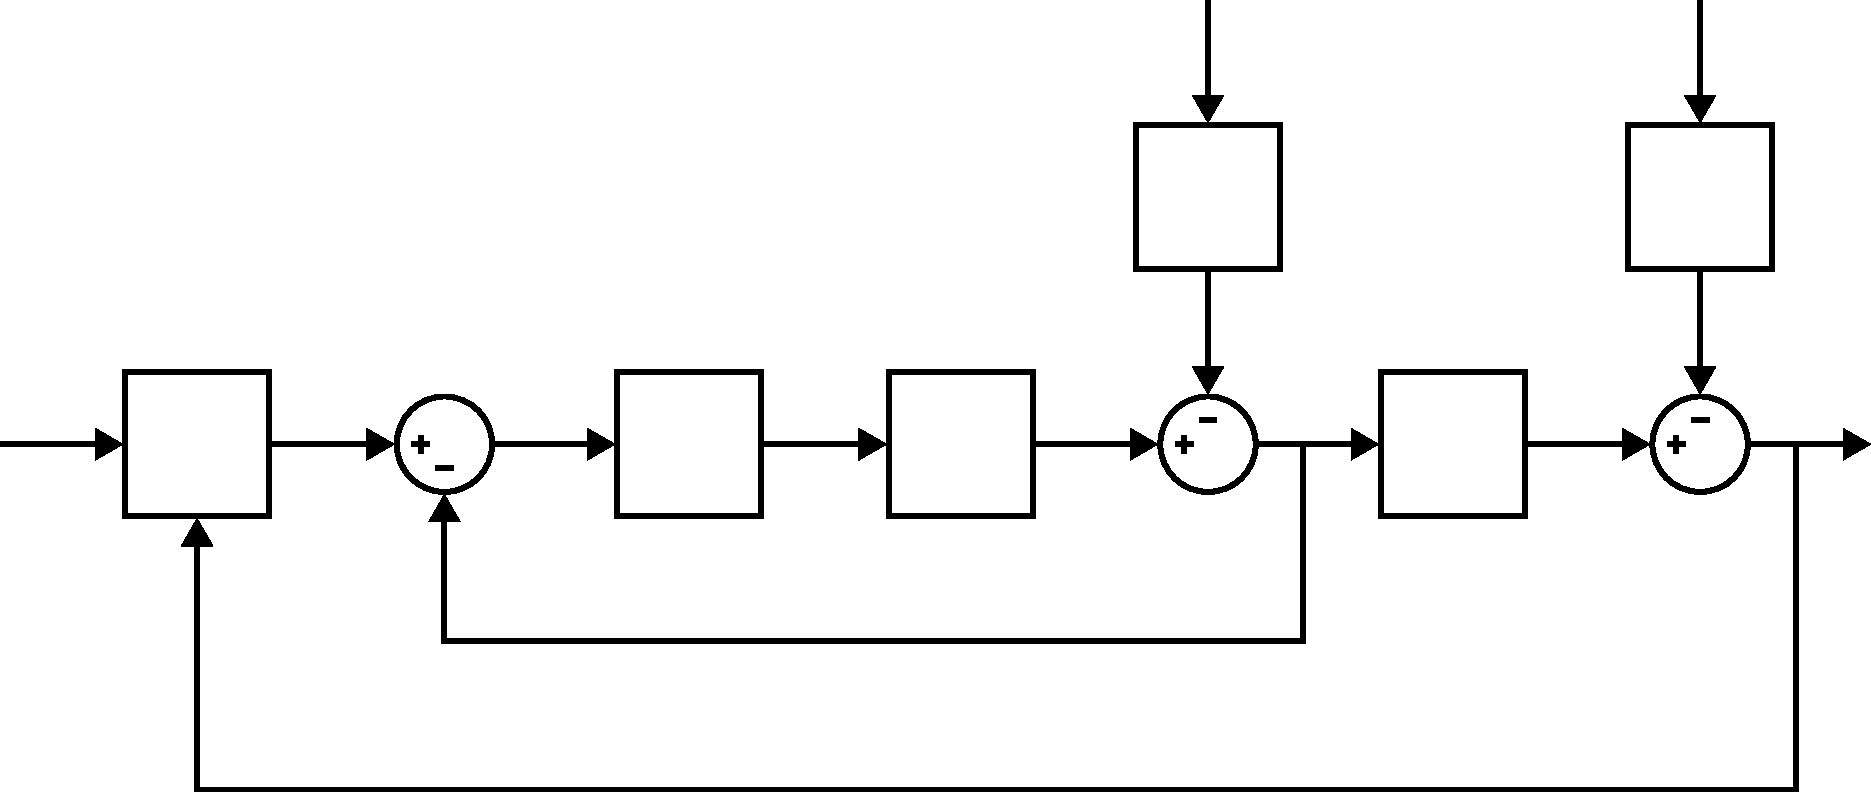
\includegraphics[width=0.9\textwidth]{img/multiloop_geral}}
            \def\svgwidth{0.9\textwidth}
            \input{./img/multiloop_geral.pdf_tex}}
        \renewcommand\figurename{Fig.}
        \caption{Estrutura geral de Controle Multimalha.}
        \label{fig:multiloop}
    \end{figure}

    A decisão sobre qual variável deve ser controlada em cada uma das malhas é complexa,
    e uma análise mais profunda deve ser feita para verificar qual a melhor
    opção para cada malha. Essa análise é feita em~\cite{ref:NASER}, utilizando o
    método do lugar das raízes e a técnica do espaço de estados médio. Esta é uma técnica
    essencial para a análise de circuitos chaveados, pois permite que as técnicas de
    análise de circuitos tradicionais sejam aplicadas a eles.

    O princípio de funcionamento é que a comutação ciclo a ciclo é ignorada em
    favor das características médias do circuito nas frequências abaixo da
    frequência de Nyquist. Perde-se então a capacidade de ver a forma de onda
    da comutação, mas pode-se determinar rapidamente uma série de fatores
    do circuito, como estabilidade, margem de ganho e de fase, o lugar das
    raízes e a resposta transiente média. Os passos para usar esta técnica são
    os seguintes:

    \begin{enumerate}
        \item Desenhar o circuito em cada estado;
        \item Escrever a equação de nó, malha ou elemento para cada estado;
        \item Determinar qual parcela do período o sistema permanece em cada estado;
        \item Multiplicar cada equação de estado por sua parcela de tempo e somá-las
            para obter uma média ponderada das equações de estado.
    \end{enumerate}

    As funções de transferência da tensão $v_c$ e da corrente $i_c$ do
    capacitor em relação à razão cíclica $d$ são dadas por:

    \begin{equation}
        \frac{v_c}{d} = \frac{\frac{2V_{DC}}{L_1} \frac{1}{C}
        	\left( s + \frac{R_2}{L_2} \right)}{s^3 + a_2 s^2 + a_1 s + a_0}
        \label{eq:vc}
    \end{equation}

    \begin{equation}
        \frac{i_c}{d} = \frac{\frac{2V_{DC}}{L_1} s
        	\left( s + \frac{R_2}{L_2} \right)}{s^3 + a_2 s^2 + a_1 s + a_0}
        \label{eq:ic}
    \end{equation}

    Com

    \begin{equation*}
        a_2 = \frac{R_1}{L_1} + \frac{R_2}{L_2}
    \end{equation*}

    \begin{equation*}
        a_1 = \frac{1}{L_1 L_2} \left( R_1 R_2 + \frac{L_1 + L_2}{C} \right)
    \end{equation*}

    \begin{equation*}
        a_0 = \frac{R_1 + R_2}{C L_1 L_2}
    \end{equation*}


    A Fig.~\ref{fig:rlocus_vc} mostra o lugar das raízes para a função de
    transferência (\ref{eq:vc}).

    \begin{figure}[htb]
        \centering{
           %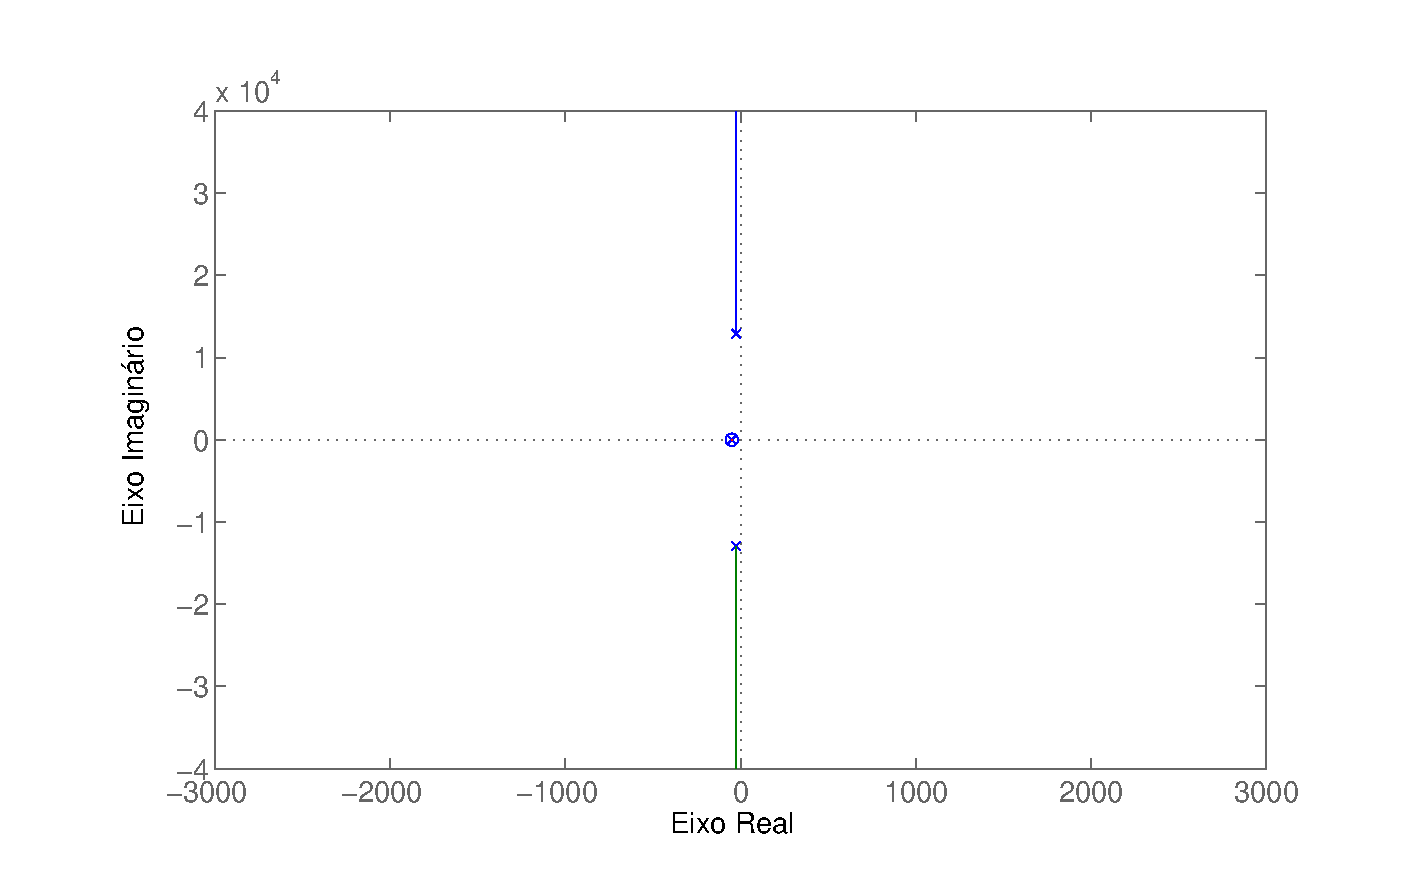
\includegraphics[width=0.9\textwidth]{img/rlocus_vc}}
           % This file was created by matlab2tikz v0.4.7 running on MATLAB 7.14.
% Copyright (c) 2008--2014, Nico Schlömer <nico.schloemer@gmail.com>
% All rights reserved.
% Minimal pgfplots version: 1.3
% 
% The latest updates can be retrieved from
%   http://www.mathworks.com/matlabcentral/fileexchange/22022-matlab2tikz
% where you can also make suggestions and rate matlab2tikz.
% 
%
% defining custom colors
\definecolor{mycolor1}{rgb}{0.66667,0.66667,0.66667}%
%
\begin{tikzpicture}

\begin{axis}[%
width=0.8\textwidth,
height=0.461611624834875\textwidth,
scale only axis,
xmin=-1.2,
xmax=1.2,
xtick={  -1, -0.5,    0,  0.5,    1},
xlabel={Eixo Real},
xmajorgrids,
ymin=-12000,
ymax=12000,
ytick={-10000,-5000,0,5000,10000},
yticklabels={{$-1$},{$-0.5$},{$0$},{$0.5$},{$1$}},
ylabel={Eixo Imaginário},
ymajorgrids
]
\addplot [color=mycolor1,line width=1.5pt,mark size=4.0pt,only marks,mark=x,mark options={solid},forget plot]
  table[row sep=crcr]{-0	5000\\
-0	5477.22557505166\\
-0	5916.07978309962\\
-0	6324.55532033676\\
-0	6708.20393249937\\
-0	7071.06781186548\\
-0	7416.19848709566\\
-0	7745.96669241484\\
-0	8062.25774829855\\
-0	8366.60026534076\\
-0	8660.25403784439\\
-0	8944.27190999916\\
-0	9219.54445729289\\
-0	9486.83298050514\\
-0	9746.79434480896\\
-0	10000\\
-0	10246.9507659596\\
-0	10488.0884817015\\
-0	10723.8052947636\\
-0	10954.4511501033\\
-0	11180.3398874989\\
-0	11401.7542509914\\
-0	11618.9500386223\\
-0	11832.1595661992\\
-0	12041.5945787923\\
};
\addplot [color=black!50!mycolor1,line width=1.5pt,mark size=4.0pt,only marks,mark=x,mark options={solid},forget plot]
  table[row sep=crcr]{0	-5000\\
0	-5477.22557505166\\
0	-5916.07978309962\\
0	-6324.55532033676\\
0	-6708.20393249937\\
0	-7071.06781186548\\
0	-7416.19848709566\\
0	-7745.96669241484\\
0	-8062.25774829855\\
0	-8366.60026534076\\
0	-8660.25403784439\\
0	-8944.27190999916\\
0	-9219.54445729289\\
0	-9486.83298050514\\
0	-9746.79434480896\\
0	-10000\\
0	-10246.9507659596\\
0	-10488.0884817015\\
0	-10723.8052947636\\
0	-10954.4511501033\\
0	-11180.3398874989\\
0	-11401.7542509914\\
0	-11618.9500386223\\
0	-11832.1595661992\\
0	-12041.5945787923\\
};
\addplot [color=black,line width=1.5pt,mark size=4.0pt,only marks,mark=o,mark options={solid},forget plot]
  table[row sep=crcr]{0	0\\
};
\end{axis}
\end{tikzpicture}%}
        \renewcommand\figurename{Fig.}
        \caption{Lugar das raízes para a tensão do capacitor.}
        \label{fig:rlocus_vc}
    \end{figure}

    Percebe-se que os polos da função de transferência da tensão do capacitor
    apresentam um comportamento oscilatório ao longo do eixo imaginário. Devido
    ao projeto do filtro \emph{LCL}, a oscilação não ocorre em uma frequência
    muito alta, o que simplifica o controle desta variável. Além disso, na prática
    haverá sempre parte real nas resistências, o que fará com que os polos desloquem-se
    um pouco para o semiplano esquerdo, saindo do limiar de estabilidade.

    Supondo que o controlador da malha interna tenha um elevado desempenho
    no rastreamento de referências e na rejeição de distúrbios,
    o controle da tensão do capacitor é vantajoso. O capacitor
    pode ser visto como uma fonte de tensão, e toda a dinâmica
    do inversor e do indutor do lado do conversor podem ser ignorados,
    simplificando o controle da corrente da rede.

    A Fig.~\ref{fig:rlocus_ic} mostra o lugar das raízes para a função de
    transferência (\ref{eq:ic}).

    \begin{figure}[htb]
        \centering{
            %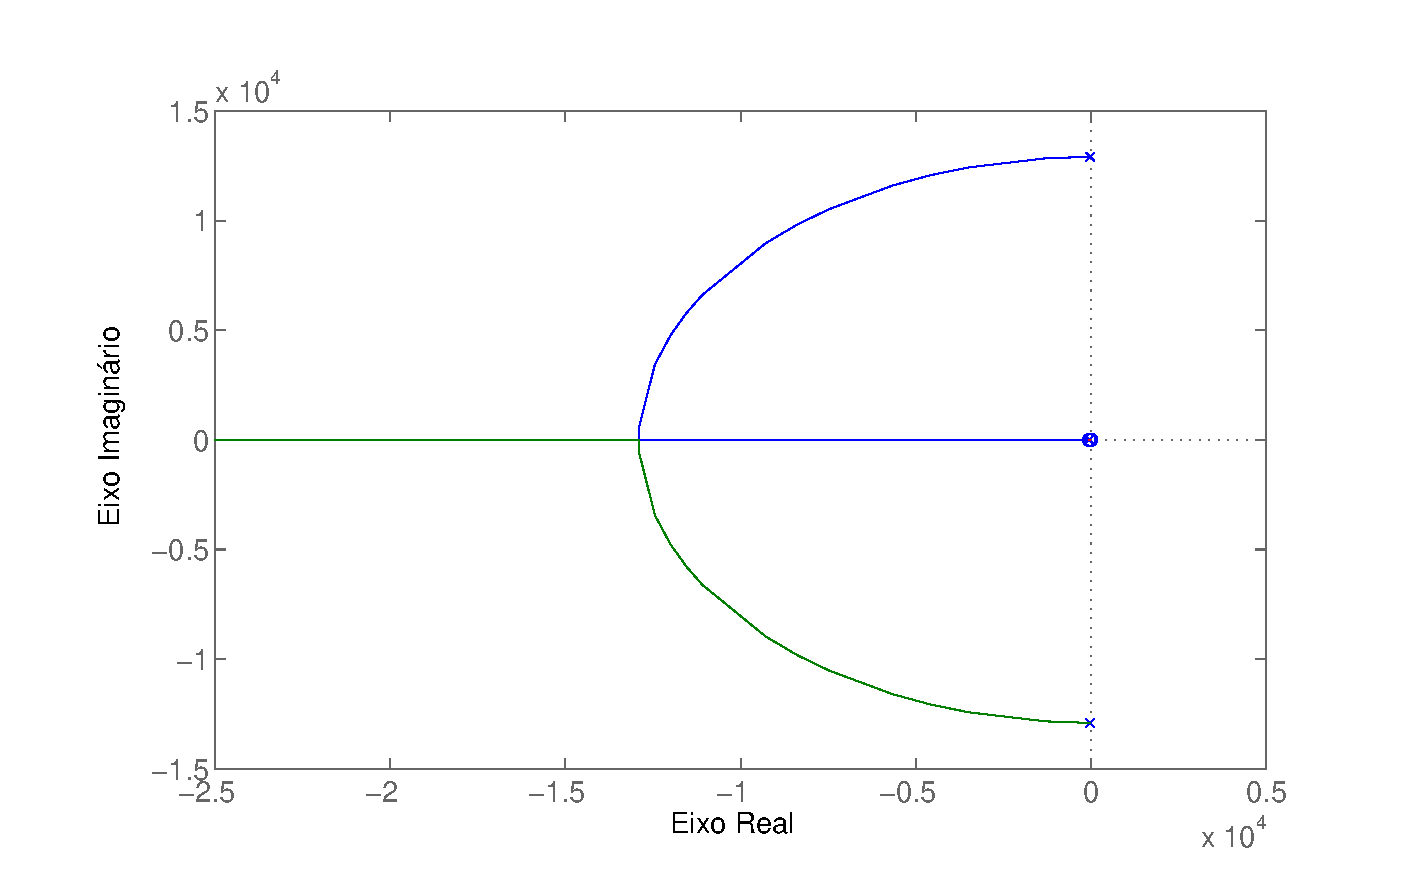
\includegraphics[width=0.9\textwidth]{img/rlocus_ic}}
            % This file was created by matlab2tikz v0.4.7 running on MATLAB 7.14.
% Copyright (c) 2008--2014, Nico Schlömer <nico.schloemer@gmail.com>
% All rights reserved.
% Minimal pgfplots version: 1.3
% 
% The latest updates can be retrieved from
%   http://www.mathworks.com/matlabcentral/fileexchange/22022-matlab2tikz
% where you can also make suggestions and rate matlab2tikz.
% 
%
% defining custom colors
\definecolor{mycolor1}{rgb}{0.33333,0.33333,0.33333}%
%
\begin{tikzpicture}

\begin{axis}[%
width=0.8\textwidth,
height=0.461611624834875\textwidth,
scale only axis,
xmin=-10000,
xmax=2000,
xtick={-8000, -4000,     0},
xlabel={Eixo Real},
xmajorgrids,
ymin=-5500,
ymax=5500,
ytick={-5000, -2500,     0,  2500,  5000},
ylabel={Eixo Imaginário},
ymajorgrids,
scaled y ticks = false,
y tick label style={/pgf/number format/.cd, fixed, fixed zerofill, precision=0},
scaled x ticks = false,
x tick label style={/pgf/number format/.cd, fixed, fixed zerofill, precision=0}
]
\addplot [color=mycolor1,line width=1.5pt,mark size=4.0pt,only marks,mark=x,mark options={solid},forget plot]
  table[row sep=crcr]{-0	5000\\
-100	4998.99989998\\
-200	4995.99839871872\\
-300	4990.99188538711\\
-400	4983.97431775085\\
-500	4974.9371855331\\
-600	4963.86945839634\\
-700	4950.75751779462\\
-800	4935.58507170123\\
-900	4918.33305094318\\
-1000	4898.97948556635\\
-1100	4877.49935930288\\
-1200	4853.86443980464\\
-1300	4828.04308182933\\
-1400	4800\\
-1500	4769.69600708473\\
-1600	4737.0877129308\\
-1700	4702.1271782035\\
-1800	4664.76151587624\\
-1900	4624.93243193887\\
-2000	4582.57569495584\\
-2100	4537.62052181537\\
-2200	4489.98886412873\\
-2300	4439.59457608462\\
-2400	4386.34243989226\\
-2500	4330.12701892219\\
-2600	4270.83130081253\\
-2700	4208.32508250016\\
-2800	4142.4630354416\\
-2900	4073.08237088326\\
-3000	4000\\
-3100	3923.00904918661\\
-3200	3841.87454245971\\
-3300	3756.32799419859\\
-3400	3666.06055596467\\
-3500	3570.71421427142\\
-3600	3469.8703145795\\
-3700	3363.03434416005\\
-3800	3249.61536185438\\
-3900	3128.8975694324\\
-4000	3000\\
-4100	2861.81760425084\\
-4200	2712.93199325011\\
-4300	2551.47016443462\\
-4400	2374.86841740758\\
-4500	2179.44947177034\\
-4600	1959.59179422654\\
-4700	1705.8722109232\\
-4800	1400\\
-4900	994.987437106622\\
-5000	0\\
-4095.01243788791	0\\
-3771.71431429143	0\\
-3542.16041687531	0\\
-3360.39219456289	0\\
-3208.71215252208	0\\
-3078.0959574163	0\\
-2963.2135633192	0\\
-2860.61230866019	0\\
-2767.90804732684	0\\
-2683.3752096446	0\\
-2605.71895806877	0\\
-2533.93944403533	0\\
-2467.24642065264	0\\
-2405.00312891236	0\\
-2346.68806854096	0\\
-2291.8681542924	0\\
-2240.17937580445	0\\
-2191.31255127883	0\\
-2145.0026288125	0\\
-2101.02051443364	0\\
-2059.16673554858	0\\
-2019.26646120455	0\\
-1981.16554121112	0\\
-1944.72732120566	0\\
-1909.83005625053	0\\
-1876.36479149833	0\\
-1844.23361121706	0\\
-1813.34818116169	0\\
-1783.62852665079	0\\
-1755.0020016016	0\\
-1727.40241345807	0\\
-1700.76927629123	0\\
-1675.04716997925	0\\
-1650.18518772552	0\\
-1626.13645756624	0\\
-1602.85772618564	0\\
-1580.30899546897	0\\
-1558.45320390733	0\\
-1537.25594632001	0\\
-1516.68522645212	0\\
-1496.71123789186	0\\
-1477.30616947687	0\\
-1458.44403195386	0\\
-1440.10050314704	0\\
-1422.25278929824	0\\
-1404.87950058085	0\\
-1387.96053907346	0\\
-1371.47699771781	0\\
-1355.41106898641	0\\
-1339.74596215561	0\\
-1324.46582822447	0\\
-1309.55569164285	0\\
-1295.00138811782	0\\
-1280.7895078576	0\\
-1266.90734369031	0\\
-1253.34284356166	0\\
-1240.08456697418	0\\
-1227.12164498054	0\\
-1214.44374338779	0\\
-1202.04102886729	0\\
-1189.90413769877	0\\
-1178.02414690596	0\\
-1166.39254756728	0\\
-1155.00122010744	0\\
-1143.84241139601	0\\
-1132.90871349638	0\\
-1122.19304392446	0\\
-1111.68862729009	0\\
-1101.3889782065	0\\
-1091.28788536429	0\\
-1081.37939667583	0\\
-1071.65780540516	0\\
-1062.11763720584	0\\
-1052.75363799657	0\\
-1043.5607626104	0\\
-1034.53416415923	0\\
-1025.66918406027	0\\
-1016.96134267565	0\\
-1008.40633052071	0\\
-1000	0\\
-991.738357633661	0\\
-983.617556739639	0\\
-975.633890540252	0\\
-967.783785663958	0\\
-960.063796015548	0\\
-952.470596990098	0\\
-945.000980007878	0\\
-937.651847349178	0\\
-930.420207269628	0\\
-923.303169377979	0\\
-916.297940259724	0\\
-909.40181933108	0\\
-902.612194909039	0\\
-895.926540484164	0\\
-889.342411183801	0\\
-882.857440414203	0\\
-876.469336670895	0\\
-870.175880507321	0\\
-863.974921652498	0\\
-857.864376269049	0\\
-851.842224343527	0\\
-845.906507201508	0\\
-840.055325140417	0\\
-834.286835173501	0\\
-828.59924887879	0\\
-822.990830347299	0\\
-817.459894225045	0\\
-812.004803843844	0\\
-806.623969436129	0\\
-801.315846429336	0\\
-796.078933815687	0\\
-790.911772593422	0\\
-785.81294427581	0\\
-780.781069464453	0\\
-775.814806483612	0\\
-770.912850072497	0\\
-766.073930132599	0\\
-761.296810527355	0\\
-756.580287931556	0\\
-751.923190728079	0\\
-747.324377949644	0\\
-742.782738263434	0\\
-738.297188996537	0\\
-733.866675200273	0\\
-729.490168751577	0\\
-725.16666748972	0\\
-720.895194386719	0\\
-716.674796749902	0\\
-712.504545455146	0\\
-708.383534209417	0\\
-704.310878841275	0\\
-700.285716618114	0\\
-696.307205588936	0\\
-692.374523951553	0\\
-688.486869443124	0\\
-684.643458753047	0\\
-680.843526957207	0\\
-677.086326972696	0\\
-673.371129032116	0\\
-669.69722017664	0\\
-666.063903767052	0\\
-662.470499012011	0\\
-658.916340512819	0\\
-655.40077782403	0\\
-651.923175029236	0\\
-648.482910331426	0\\
-645.079375657321	0\\
-641.711976275124	0\\
-638.380130425167	0\\
-635.083268962916	0\\
-631.820835013871	0\\
-628.592283639892	0\\
-625.397081516486	0\\
-622.234706620669	0\\
-619.104647928957	0\\
-616.006405125126	0\\
-612.939488317361	0\\
-609.903417764441	0\\
-606.897723610616	0\\
-603.921945628861	0\\
-600.975632972188	0\\
-598.058343932725	0\\
-595.169645708275	0\\
-592.309114176076	0\\
-589.476333673516	0\\
-586.670896785536	0\\
-583.892404138494	0\\
-581.14046420025	0\\
-578.414693086257	0\\
-575.71471437145	0\\
-573.040158907715	0\\
-570.390664646761	0\\
-567.7658764682	0\\
-565.165446012649	0\\
-562.589031519695	0\\
-560.036297670543	0\\
-557.5069154352	0\\
-555.000561924035	0\\
-552.516920243569	0\\
-550.055679356352	0\\
-547.616533944799	0\\
-545.199184278843	0\\
-542.803336087285	0\\
-540.428700432722	0\\
-538.074993589932	0\\
-535.741936927605	0\\
-533.429256793314	0\\
-531.136684401621	0\\
-528.863955725216	0\\
-526.610811388995	0\\
-524.376996566984	0\\
-522.162260882013	0\\
-519.966358308069	0\\
-517.789047075227	0\\
-515.630089577087	0\\
-513.489252280645	0\\
-511.36630563851	0\\
-509.261024003407	0\\
-507.173185544895	0\\
-505.102572168219	0\\
-503.048969435256	0\\
-501.01216648747	0\\
-498.991955970822	0\\
-496.988133962591	0\\
-495.000499900025	0\\
-493.028856510788	0\\
-491.073009745139	0\\
-489.132768709801	0\\
-487.207945603458	0\\
-485.298355653853	0\\
-483.403817056412	0\\
-481.524150914386	0\\
-479.659181180431	0\\
-477.808734599615	0\\
-475.972640653791	0\\
-474.15073150731	0\\
-472.34284195403	0\\
-470.548809365585	0\\
-468.768473640885	0\\
-467.001677156801	0\\
-465.248264720018	0\\
-463.508083520007	0\\
-461.780983083099	0\\
-460.066815227622	0\\
-458.36543402008	0\\
-456.676695732337	0\\
-455.000458799784	0\\
-453.336583780463	0\\
-451.684933315123	0\\
-450.045372088178	0\\
-448.417766789547	0\\
-446.801986077352	0\\
-445.197900541458	0\\
-443.605382667814	0\\
-442.0243068036	0\\
-440.454549123134	0\\
-438.89598759454	0\\
-437.348501947142	0\\
-435.811973639578	0\\
-434.2862858286	0\\
-432.77132333856	0\\
-431.266972631555	0\\
-429.773121778208	0\\
-428.28966042909	0\\
-426.816479786738	0\\
-425.353472578284	0\\
-423.900533028653	0\\
-422.457556834336	0\\
-421.024441137714	0\\
-419.60108450192	0\\
-418.187386886225	0\\
-416.783249621944	0\\
-415.388575388838	0\\
-414.003268192001	0\\
-412.627233339233	0\\
-411.260377418868	0\\
-409.902608278064	0\\
-408.553835001533	0\\
-407.2139678907	0\\
-405.882918443291	0\\
-404.560599333327	0\\
-403.246924391526	0\\
-401.941808586094	0\\
-400.645168003899	0\\
-399.356919832027	0\\
-398.076982339694	0\\
-396.805274860523	0\\
-395.541717775166	0\\
-394.286232494272	0\\
-393.038741441783	0\\
-391.799168038562	0\\
-390.567436686331	0\\
-389.343472751928	0\\
-388.127202551863	0\\
-386.918553337177	0\\
-385.717453278585	0\\
-384.523831451903	0\\
-383.337617823762	0\\
-382.158743237582	0\\
-380.987139399819	0\\
-379.822738866466	0\\
-378.665475029813	0\\
-377.515282105453	0\\
-376.372095119531	0\\
-375.235849896229	0\\
-374.106483045486	0\\
-372.983931950943	0\\
-371.868134758114	0\\
-370.759030362766	0\\
-369.656558399526	0\\
-368.560659230683	0\\
-367.471273935198	0\\
-366.388344297921	0\\
-365.31181279899	0\\
-364.241622603432	0\\
-363.177717550947	0\\
-362.120042145875	0\\
-361.068541547344	0\\
-360.02316155959	0\\
-358.983848622454	0\\
-357.950549802045	0\\
-356.923212781567	0\\
-355.901785852307	0\\
-354.886217904785	0\\
-353.876458420055	0\\
-352.872457461161	0\\
-351.874165664738	0\\
-350.881534232759	0\\
-349.894514924432	0\\
-348.913060048225	0\\
-347.937122454039	0\\
-346.966655525505	0\\
-346.001613172423	0\\
-345.041949823323	0\\
-344.087620418151	0\\
-343.138580401088	0\\
-342.194785713481	0\\
-341.256192786894	0\\
-340.322758536284	0\\
-339.39444035328	0\\
-338.471196099583	0\\
-337.552984100472	0\\
-336.639763138417	0\\
-335.731492446799	0\\
-334.828131703736	0\\
-333.929641026007	0\\
-333.035980963077	0\\
-332.14711249122	0\\
-331.262997007738	0\\
-330.383596325274	0\\
-329.508872666217	0\\
-328.6387886572	0\\
-327.77330732368	0\\
-326.912392084616	0\\
-326.05600674722	0\\
-325.204115501805	0\\
-324.356682916702	0\\
-323.513673933271	0\\
-322.675053860979	0\\
-321.840788372568	0\\
-321.010843499286	0\\
-320.185185626205	0\\
-319.363781487609	0\\
-318.546598162448	0\\
-317.73360306987	0\\
-316.924763964825	0\\
-316.120048933726	0\\
-315.319426390189	0\\
-314.522865070832	0\\
-313.730334031141	0\\
-312.941802641402	0\\
-312.157240582689	0\\
-311.376617842919	0\\
-310.599904712967	0\\
-309.827071782834	0\\
-309.058089937882	0\\
-308.292930355122	0\\
-307.531564499553	0\\
-306.773964120565	0\\
-306.020101248391	0\\
-305.269948190612	0\\
-304.523477528716	0\\
-303.780662114708	0\\
-303.041475067769	0\\
-302.305889770966	0\\
-301.573879868013	0\\
-300.845419260069	0\\
-300.120482102602	0\\
-299.399042802278	0\\
-298.681076013915	0\\
-297.966556637463	0\\
-297.255459815046	0\\
-296.547760928031	0\\
-295.843435594153	0\\
-295.14245966467	0\\
-294.444809221567	0\\
-293.7504605748	0\\
-293.059390259571	0\\
-292.371575033656	0\\
-291.686991874755	0\\
-291.005617977897	0\\
-290.327430752865	0\\
-289.652407821673	0\\
-288.980527016065	0\\
-288.311766375061	0\\
-287.646104142527	0\\
-286.98351876479	0\\
-286.323988888275	0\\
-285.667493357187	0\\
-285.014011211213	0\\
-284.363521683267	0\\
-283.716004197259	0\\
-283.071438365898	0\\
-282.429803988525	0\\
-281.791081048975	0\\
-281.155249713469	0\\
-280.522290328537	0\\
-279.892183418962	0\\
-279.264909685766	0\\
-278.640450004206	0\\
-278.018785421812	0\\
-277.399897156442	0\\
-276.783766594373	0\\
-276.170375288402	0\\
-275.559704955994	0\\
-274.951737477433	0\\
-274.346454894014	0\\
-273.743839406254	0\\
-273.143873372121	0\\
-272.546539305297	0\\
-271.951819873454	0\\
-271.359697896564	0\\
-270.770156345218	0\\
-270.18317833898	0\\
-269.598747144753	0\\
-269.016846175172	0\\
-268.437458987017	0\\
-267.860569279645	0\\
-267.286160893445	0\\
-266.71421780831	0\\
-266.14472414213	0\\
-265.577664149311	0\\
-265.0130222193	0\\
-264.45078287514	0\\
-263.890930772039	0\\
-263.333450695961	0\\
-262.778327562226	0\\
-262.225546414144	0\\
-261.675092421648	0\\
-261.126950879957	0\\
-260.581107208252	0\\
-260.037546948371	0\\
-259.496255763512	0\\
-258.957219436968	0\\
-258.420423870862	0\\
-257.885855084906	0\\
-257.353499215178	0\\
-256.823342512905	0\\
-256.295371343272	0\\
-255.769572184238	0\\
-255.24593162537	0\\
-254.72443636669	0\\
-254.205073217541	0\\
-253.687829095457	0\\
-253.172691025059	0\\
-252.659646136956	0\\
-252.148681666662	0\\
-251.639784953529	0\\
-251.132943439686	0\\
-250.628144669002	0\\
-250.12537628605	0\\
-249.624626035091	0\\
-249.125881759068	0\\
-248.629131398611	0\\
-248.134362991059	0\\
-247.641564669486	0\\
-247.150724661744	0\\
-246.661831289519	0\\
-246.174872967392	0\\
-245.689838201918	0\\
-245.206715590712	0\\
-244.725493821545	0\\
-244.246161671455	0\\
-243.768708005864	0\\
-243.293121777712	0\\
-242.819392026591	0\\
-242.347507877898	0\\
-241.877458541996	0\\
-241.409233313381	0\\
-240.942821569866	0\\
-240.478212771765	0\\
-240.015396461096	0\\
-239.554362260786	0\\
-239.09509987389	0\\
-238.637599082819	0\\
-238.181849748571	0\\
-237.727841809977	0\\
-237.275565282958	0\\
-236.825010259778	0\\
-236.376166908323	0\\
-235.929025471374	0\\
-235.483576265893	0\\
-235.039809682322	0\\
-234.597716183883	0\\
-234.157286305889	0\\
-233.718510655064	0\\
-233.281379908866	0\\
-232.845884814825	0\\
-232.412016189884	0\\
-231.979764919743	0\\
-231.549121958222	0\\
-231.120078326621	0\\
-230.69262511309	0\\
-230.266753472009	0\\
-229.84245462337	0\\
-229.419719852171	0\\
-228.998540507813	0\\
-228.578908003504	0\\
-228.160813815674	0\\
-227.744249483389	0\\
-227.329206607776	0\\
-226.915676851458	0\\
-226.503651937986	0\\
-226.093123651285	0\\
-225.684083835104	0\\
-225.276524392467	0\\
-224.870437285142	0\\
-224.4658145331	0\\
-224.062648213995	0\\
-223.660930462638	0\\
-223.260653470482	0\\
-222.861809485115	0\\
-222.464390809754	0\\
-222.068389802745	0\\
-221.673798877067	0\\
-221.280610499851	0\\
-220.888817191891	0\\
-220.498411527166	0\\
-220.109386132369	0\\
-219.72173368644	0\\
-219.335446920102	0\\
-218.950518615402	0\\
-218.566941605259	0\\
-218.184708773017	0\\
-217.803813052	0\\
-217.424247425073	0\\
-217.046004924208	0\\
-216.669078630055	0\\
-216.293461671519	0\\
-215.919147225332	0\\
-215.546128515646	0\\
-215.174398813615	0\\
-214.803951436989	0\\
-214.434779749712	0\\
-214.066877161519	0\\
-213.700237127546	0\\
-213.334853147936	0\\
-212.970718767452	0\\
-212.607827575095	0\\
-212.246173203726	0\\
-211.885749329687	0\\
-211.526549672435	0\\
-211.168567994171	0\\
-210.811798099478	0\\
-210.456233834958	0\\
-210.101869088881	0\\
-209.748697790829	0\\
-209.396713911345	0\\
-209.045911461593	0\\
-208.69628449301	0\\
-208.347827096972	0\\
-208.000533404456	0\\
-207.65439758571	0\\
-207.309413849924	0\\
-206.965576444902	0\\
-206.622879656746	0\\
-206.281317809532	0\\
-205.940885264998	0\\
-205.601576422227	0\\
-205.263385717345	0\\
-204.926307623209	0\\
-204.590336649103	0\\
-204.255467340444	0\\
-203.92169427848	0\\
-203.589012079998	0\\
-203.257415397028	0\\
-202.926898916563	0\\
-202.597457360266	0\\
-202.269085484189	0\\
-201.941778078496	0\\
-201.615529967182	0\\
-201.290336007799	0\\
-200.966191091185	0\\
-200.643090141197	0\\
-200.321028114439	0\\
-200	0\\
-199.680000819196	0\\
-199.361025625306	0\\
-199.043069503317	0\\
-198.726127569673	0\\
-198.410194972019	0\\
-198.095266888954	0\\
-197.781338529784	0\\
-197.468405134277	0\\
-197.156461972421	0\\
-196.845504344186	0\\
-196.535527579285	0\\
-196.226527036936	0\\
-195.918498105634	0\\
-195.611436202917	0\\
-195.305336775139	0\\
-195.000195297243	0\\
-194.696007272534	0\\
-194.392768232462	0\\
-194.090473736397	0\\
-193.789119371414	0\\
-193.488700752077	0\\
-193.18921352022	0\\
-192.890653344744	0\\
-192.593015921398	0\\
-192.296296972576	0\\
-192.00049224711	0\\
-191.705597520065	0\\
-191.411608592538	0\\
-191.118521291455	0\\
-190.826331469375	0\\
-190.535035004293	0\\
-190.244627799442	0\\
-189.955105783104	0\\
-189.666464908416	0\\
-189.378701153181	0\\
-189.09181051968	0\\
-188.805789034487	0\\
-188.520632748282	0\\
-188.23633773567	0\\
-187.952900095001	0\\
-187.670315948187	0\\
-187.388581440526	0\\
-187.107692740528	0\\
-186.827646039737	0\\
-186.548437552558	0\\
-186.270063516088	0\\
-185.992520189945	0\\
-185.715803856097	0\\
-185.4399108187	0\\
-185.164837403926	0\\
-184.890579959807	0\\
-184.617134856065	0\\
-184.344498483957	0\\
-184.072667256109	0\\
-183.801637606364	0\\
-183.531405989623	0\\
-183.261968881687	0\\
-182.993322779106	0\\
-182.725464199027	0\\
-182.45838967904	0\\
-182.192095777028	0\\
-181.926579071021	0\\
-181.661836159047	0\\
-181.397863658986	0\\
-181.134658208425	0\\
-180.872216464514	0\\
-180.610535103827	0\\
-180.349610822217	0\\
-180.089440334677	0\\
-179.830020375202	0\\
-179.571347696654	0\\
-179.313419070622	0\\
-179.056231287288	0\\
-178.799781155294	0\\
-178.544065501611	0\\
-178.289081171403	0\\
-178.0348250279	0\\
-177.781293952268	0\\
-177.528484843481	0\\
-177.276394618193	0\\
-177.025020210612	0\\
-176.774358572378	0\\
-176.524406672433	0\\
-176.275161496907	0\\
-176.026620048986	0\\
-175.778779348802	0\\
-175.531636433303	0\\
-175.285188356142	0\\
-175.039432187556	0\\
-174.794365014251	0\\
-174.549983939283	0\\
-174.306286081948	0\\
-174.063268577663	0\\
-173.820928577859	0\\
-173.579263249864	0\\
-173.338269776795	0\\
-173.097945357448	0\\
-172.858287206187	0\\
-172.619292552838	0\\
-172.380958642579	0\\
-172.14328273584	0\\
-171.906262108187	0\\
-171.669894050228	0\\
-171.434175867502	0\\
-171.199104880382	0\\
-170.964678423966	0\\
-170.730893847982	0\\
-170.497748516684	0\\
-170.265239808756	0\\
-170.033365117208	0\\
-169.802121849284	0\\
-169.571507426361	0\\
-169.341519283852	0\\
-169.112154871116	0\\
-168.883411651356	0\\
-168.655287101532	0\\
-168.427778712261	0\\
-168.20088398773	0\\
-167.974600445603	0\\
-167.748925616928	0\\
-167.523857046048	0\\
-167.299392290513	0\\
-167.075528920989	0\\
-166.852264521172	0\\
-166.629596687698	0\\
-166.40752303006	0\\
-166.186041170517	0\\
-165.965148744016	0\\
-165.7448433981	0\\
-165.525122792828	0\\
-165.305984600692	0\\
-165.087426506534	0\\
-164.869446207462	0\\
-164.652041412772	0\\
-164.435209843866	0\\
-164.21894923417	0\\
-164.00325732906	0\\
-163.788131885776	0\\
-163.573570673352	0\\
-163.359571472531	0\\
-163.146132075693	0\\
-162.933250286777	0\\
-162.720923921208	0\\
-162.509150805816	0\\
-162.297928778767	0\\
-162.087255689488	0\\
-161.877129398592	0\\
-161.667547777807	0\\
-161.458508709902	0\\
-161.250010088618	0\\
-161.042049818596	0\\
-160.834625815303	0\\
-160.627736004968	0\\
-160.42137832451	0\\
-160.215550721466	0\\
-160.010251153928	0\\
-159.805477590472	0\\
-159.601228010091	0\\
-159.39750040213	0\\
-159.194292766217	0\\
-158.991603112199	0\\
-158.789429460078	0\\
-158.587769839942	0\\
-158.386622291905	0\\
-158.185984866043	0\\
-157.985855622328	0\\
-157.786232630566	0\\
-157.587113970337	0\\
-157.388497730931	0\\
-157.190382011287	0\\
-156.992764919932	0\\
-156.795644574923	0\\
-156.599019103781	0\\
-156.40288664344	0\\
-156.20724534018	0\\
-156.012093349572	0\\
-155.817428836421	0\\
-155.623249974706	0\\
-155.429554947523	0\\
-155.236341947029	0\\
-155.043609174385	0\\
-154.851354839701	0\\
-154.659577161977	0\\
-154.468274369053	0\\
-154.277444697549	0\\
-154.087086392814	0\\
-153.897197708872	0\\
-153.707776908367	0\\
-153.518822262508	0\\
-153.330332051023	0\\
-153.142304562097	0\\
-152.954738092328	0\\
-152.767630946673	0\\
-152.580981438395	0\\
-152.394787889012	0\\
-152.20904862825	0\\
-152.02376199399	0\\
-151.838926332219	0\\
-151.65453999698	0\\
-151.470601350323	0\\
-151.287108762259	0\\
-151.104060610707	0\\
-150.921455281449	0\\
-150.739291168083	0\\
-150.557566671975	0\\
-150.376280202208	0\\
-150.195430175544	0\\
-150.015015016369	0\\
-149.835033156653	0\\
-149.655483035901	0\\
-149.476363101111	0\\
-149.297671806724	0\\
-149.119407614585	0\\
-148.941568993895	0\\
-148.764154421169	0\\
-148.587162380191	0\\
-148.410591361972	0\\
-148.234439864704	0\\
-148.058706393722	0\\
-147.883389461457	0\\
-147.708487587399	0\\
-147.533999298048	0\\
-147.359923126878	0\\
-147.186257614297	0\\
-147.0130013076	0\\
-146.840152760932	0\\
-146.66771053525	0\\
-146.495673198278	0\\
-146.324039324469	0\\
-146.152807494969	0\\
-145.981976297571	0\\
-145.811544326684	0\\
-145.641510183286	0\\
-145.471872474892	0\\
-145.302629815513	0\\
-145.133780825619	0\\
-144.965324132102	0\\
-144.797258368235	0\\
-144.62958217364	0\\
-144.462294194249	0\\
-144.295393082265	0\\
-144.128877496131	0\\
-143.962746100488	0\\
-143.796997566144	0\\
-143.631630570036	0\\
-143.466643795194	0\\
-143.30203593071	0\\
-143.137805671696	0\\
-142.973951719258	0\\
-142.810472780455	0\\
-142.647367568268	0\\
-142.484634801563	0\\
-142.322273205064	0\\
-142.160281509311	0\\
-141.998658450634	0\\
-141.837402771116	0\\
-141.67651321856	0\\
-141.515988546461	0\\
-141.355827513967	0\\
-141.196028885853	0\\
-141.036591432485	0\\
-140.877513929792	0\\
-140.71879515923	0\\
-140.560433907755	0\\
-140.402428967789	0\\
-140.244779137193	0\\
-140.087483219231	0\\
-139.930540022545	0\\
-139.77394836112	0\\
-139.617707054258	0\\
-139.461814926547	0\\
-139.306270807831	0\\
-139.151073533178	0\\
-138.996221942858	0\\
-138.841714882306	0\\
-138.687551202098	0\\
-138.533729757922	0\\
-138.380249410547	0\\
-138.227109025799	0\\
-138.074307474529	0\\
-137.921843632586	0\\
-137.769716380791	0\\
-137.61792460491	0\\
-137.466467195622	0\\
-137.315343048499	0\\
-137.164551063972	0\\
-137.01409014731	0\\
-136.86395920859	0\\
-136.71415716267	0\\
-136.564682929168	0\\
-136.415535432428	0\\
-136.266713601502	0\\
-136.118216370119	0\\
-135.97004267666	0\\
-135.822191464137	0\\
-135.674661680163	0\\
-135.527452276927	0\\
-135.380562211172	0\\
-135.23399044417	0\\
-135.087735941695	0\\
-134.941797673999	0\\
-134.796174615792	0\\
-134.650865746212	0\\
-134.505870048804	0\\
-134.361186511497	0\\
-134.216814126579	0\\
-134.072751890673	0\\
-133.928998804715	0\\
-133.785553873932	0\\
-133.642416107816	0\\
-133.499584520102	0\\
-133.357058128746	0\\
-133.214835955904	0\\
-133.072917027906	0\\
-132.931300375236	0\\
-132.78998503251	0\\
-132.648970038453	0\\
-132.508254435877	0\\
-132.367837271661	0\\
-132.227717596727	0\\
-132.087894466021	0\\
-131.94836693849	0\\
-131.809134077061	0\\
-131.67019494862	0\\
-131.531548623993	0\\
-131.393194177922	0\\
-131.255130689046	0\\
-131.117357239882	0\\
-130.979872916803	0\\
-130.842676810015	0\\
-130.705768013542	0\\
-130.569145625205	0\\
-130.432808746598	0\\
-130.296756483073	0\\
-130.160987943717	0\\
-130.025502241336	0\\
-129.890298492432	0\\
-129.755375817186	0\\
-129.620733339438	0\\
-129.486370186667	0\\
-129.352285489977	0\\
-129.21847838407	0\\
-129.084948007234	0\\
-128.951693501324	0\\
-128.818714011739	0\\
-128.686008687407	0\\
-128.553576680768	0\\
-128.421417147753	0\\
-128.289529247767	0\\
-128.157912143673	0\\
-128.026565001772	0\\
-127.895486991784	0\\
-127.764677286835	0\\
-127.634135063436	0\\
-127.503859501467	0\\
-127.373849784159	0\\
-127.244105098078	0\\
-127.114624633108	0\\
-126.985407582431	0\\
-126.856453142515	0\\
-126.727760513094	0\\
-126.599328897152	0\\
-126.471157500908	0\\
-126.343245533798	0\\
-126.215592208459	0\\
-126.088196740712	0\\
-125.96105834955	0\\
-125.834176257114	0\\
-125.707549688687	0\\
-125.58117787267	0\\
-125.455060040571	0\\
-125.329195426986	0\\
-125.203583269587	0\\
-125.078222809105	0\\
};
\addplot [color=white!50!mycolor1,line width=1.5pt,mark size=4.0pt,only marks,mark=x,mark options={solid},forget plot]
  table[row sep=crcr]{0	-5000\\
-100	-4998.99989998\\
-200	-4995.99839871872\\
-300	-4990.99188538711\\
-400	-4983.97431775085\\
-500	-4974.9371855331\\
-600	-4963.86945839634\\
-700	-4950.75751779462\\
-800	-4935.58507170123\\
-900	-4918.33305094318\\
-1000	-4898.97948556635\\
-1100	-4877.49935930288\\
-1200	-4853.86443980464\\
-1300	-4828.04308182933\\
-1400	-4800\\
-1500	-4769.69600708473\\
-1600	-4737.0877129308\\
-1700	-4702.1271782035\\
-1800	-4664.76151587624\\
-1900	-4624.93243193887\\
-2000	-4582.57569495584\\
-2100	-4537.62052181537\\
-2200	-4489.98886412873\\
-2300	-4439.59457608462\\
-2400	-4386.34243989226\\
-2500	-4330.12701892219\\
-2600	-4270.83130081253\\
-2700	-4208.32508250016\\
-2800	-4142.4630354416\\
-2900	-4073.08237088326\\
-3000	-4000\\
-3100	-3923.00904918661\\
-3200	-3841.87454245971\\
-3300	-3756.32799419859\\
-3400	-3666.06055596467\\
-3500	-3570.71421427142\\
-3600	-3469.8703145795\\
-3700	-3363.03434416005\\
-3800	-3249.61536185438\\
-3900	-3128.8975694324\\
-4000	-3000\\
-4100	-2861.81760425084\\
-4200	-2712.93199325011\\
-4300	-2551.47016443462\\
-4400	-2374.86841740758\\
-4500	-2179.44947177034\\
-4600	-1959.59179422654\\
-4700	-1705.8722109232\\
-4800	-1400\\
-4900	-994.987437106622\\
-5000	0\\
-6104.98756211209	0\\
-6628.28568570857	0\\
-7057.83958312469	0\\
-7439.60780543711	0\\
-7791.28784747792	0\\
-8121.9040425837	0\\
-8436.78643668081	0\\
-8739.38769133981	0\\
-9032.09195267317	0\\
-9316.6247903554	0\\
-9594.28104193123	0\\
-9866.06055596467	0\\
-10132.7535793474	0\\
};
\addplot [color=black,line width=1.5pt,mark size=4.0pt,only marks,mark=o,mark options={solid},forget plot]
  table[row sep=crcr]{0	0\\
};
\end{axis}
\end{tikzpicture}%}
        \renewcommand\figurename{Fig.}
        \caption{Lugar das raízes para a corrente do capacitor.}
        \label{fig:rlocus_ic}
    \end{figure}

    Percebe-se que os polos da função de transferência da corrente do capacitor
    deslocam-se para o semiplano esquerdo, indicando que o sistema tende à
    estabilidade. Essa é a grande vantagem de utilizar a corrente do capacitor
    como variável de controle da malha interna.

    A corrente do capacitor mostra-se como uma ótima escolha. No entanto, a tensão
    do capacitor pode ser selecionada como uma variável intermediária a ser controlada,
    sintetizando-se assim uma fonte de tensão controlada por tensão, no caso, o
    conversor. Deste modo, tem-se um circuito do tipo \emph{RL} que aproxima o
    comportamento no ponto de conexão.

    %Dessa forma, embora a corrente ofereça mais estabilidade, a tensão do capacitor
    %é escolhida como variável de controle da malha interna na presença de um controlador
    %adaptativo na malha externa, devido ao quanto essa escolha facilita a realização do
    %controle da dinâmica do filtro. Outras topologias para a malha externa serão
    %avaliadas, e então a corrente do capacitor será utilizada como variável de
    %controle para a malha interna.


\section{Objetivos e Contribuições da Dissertação}

	O objetivo desse trabalho é propor uma estratégia de controle para um conversor
	conectado à rede elétrica através de um filtro LCL. A estratégia proposta deve
	ser robusta com relação às incertezas e distúrbios da rede elétrica, e resultar
	numa dinâmica de malha fechada rápida o suficiente para permitir a rejeição de
	distúrbios e o rastreamento de possíveis referências complexas, incluindo harmônicas.

	Mais especificamente, esta Dissertação visa:

	\begin{itemize}
		\item Propor um controlador adaptativo para controlar a corrente de conversores
			conectados à rede elétrica com um filtro LCL que ajuste automaticamente os
			ganhos e que garanta estabilidade para uma ampla faixa de valores de
			impedância da rede;
		\item Propor um controlador que garanta desempenho e estabilidade frente a
			distúrbios de tensão e incerteza na impedância da rede elétrica;
		\item Realizar a prova de estabilidade do controlador proposto.
	\end{itemize}


\section{Organização do Documento}

	O Capítulo 1 apresenta a motivação para este trabalho. É apresentada uma breve
	revisão bibliográfica, de modo a situar o trabalho desenvolvido no contexto atual
	de utilização de conversores conectados à rede elétrica.

	O Capítulo 2 apresenta a modelagem matemática do sistema. O filtro LCL é modelado
	tanto em tempo contínuo quanto em tempo discreto, considerando como variável
	intermediária tanto a corrente como a tensão do capacitor.

	O Capítulo 3 apresenta a proposta de controlador adaptativo utilizando uma
	estrutura multimalha, novamente para ambos os casos de escolha de variável
	intermediária.

	O Capítulo 4 apresenta a prosposta de controlador adaptativo através de
	modelo interno.

	O Capítulo 5 apresenta os resultados obtidos com os controladores propostos,
	tanto em simulação quanto em experimentos de bancada.

	O Capítulo 6 traz as conclusões do trabalho e sugestões de trabalhos futuros.

%FIM---------------------------------------------------------------------------
